\documentclass{book}
\usepackage{titlesec}
\setcounter{secnumdepth}{4}
\usepackage{titlepic}
\usepackage{graphicx}
\titleformat{\subsubsection}
{\normalfont\normalsize\bfseries}{\theparagraph}{1em}{}
\titlespacing*{\subsubsection}
{0pt}{3.25ex plus 1ex minus .2ex}{1.5ex plus .2ex}
\usepackage{graphicx}
\graphicspath{ {images/} }
\usepackage{hyperref}
\usepackage{float}
\usepackage{listings}
\usepackage{xcolor}
\hypersetup{
    colorlinks,
    linkcolor={black!50!black},
    citecolor={black!50!black},
    urlcolor={black!50!black}
}
\begin{document}
\begin{titlepage}
	\centering
	
\includegraphics[width=0.55\textwidth]{../R/photos/aueb.png}\par\vspace{1cm}
	{\scshape\LARGE Athens University of Economics and Business, Department of Management Science and Technology\par}
	\vspace{1cm}
	{\scshape\Large Master in Business Analytics Thesis\par}
	\vspace{1.5cm}
	{\huge\bfseries Metrics of successful websites and companies\par}
	\vspace{2cm}
	{\Large\itshape Danai Avratoglou\par}
	\vfill
	supervised by\par
	Professor Spinellis D. 

	\vfill

% Bottom of the page
	{\large \today\par}
\end{titlepage}


\newpage
\begin{center}
\textbf{CERTIFICATION OF THESIS DECLARATION}
\end{center}
This paper is submitted by the author as part of mandatory procedure of the Master in Business Analytics program from the department of Management Science and Technology of the Athens University of Business and Economics and it is available in the Electronic Library of the Athens University of Economics and Business.\\\\
I hereby declare that this particular thesis has been written by me, in order  to obtain the Postgraduate Degree in Business Analytics, and has not been submitted to or approved by any other postgraduate or undergraduate program in Greece or abroad. This thesis presents my personal views on the subject. All the sources I have used for the preparation of this particular thesis are mentioned explicitly with  references being made either to their authors or to the URL’s (if found on the internet).\\\\\\\\\\
\textbf{STUDENT'S FULL NAME}
..............................................\\\\\\\\
\textbf{SIGNATURE}
........................................................................\\
\newpage
\begin{center}
\textbf{THANK YOU NOTE}
\end{center}
This thesis, it would be impossible, without the contribution and assistance of many individuals. I would like to thank all the teachers of the Master in Business Analytics program for the knowledge they have given me throughout the course of my studies. Especially I would like to thank my supervisor, professor Diomidis Spinellis for his valuable guidance in choosing the particular topic and all the helpful tips when drawing the entire work.\\
Additionally, I would like to thank all my fellow students, but especially the members of my group, which embellish all the experience in the graduate program. \\
Finally, I would like to thank Nick, my friends, and family, my mother, my sister, and finally my father, who unfortunately is no longer with us. Thanks to them I was able to achieve another one of my goals.
\newpage
\begin{center}
\textbf{Abstract}
\end{center}
In the global on line environment, comprehending the practises of websites adoptions by enterprises is becoming increasingly important. This study investigates the correlation of the implementation of specific websites metrics to a company's home page, with the revenues of U.S.A.'s most successful companies. The metrics that are examined are related to the website's quality and usability as well as to the user's satisfaction. The companies that are under examination are taken from the Fortune 500 list of 2016. The results indicate that regardless the industry that a firm belongs to there are specific metrics that can influence the success of an enterprise (in terms of its revenue) with the implementation or the avoidance of their usage. Detailed findings are presented.
\newpage
\tableofcontents
\newpage
\chapter{Introduction}

Over the past two decades, the uncanny growth of the World Wide Web (the Web or WWW), along with the expansion of the users that have access to this medium attracted the attention of enterprises and organisations. The popularity of the Web has created new opportunities for companies to attract new customers or even retain their existing ones through their websites.\\ 
Even though before the expansion of the Web the on-line presence of a company was not an important factor in the overall success that the enterprise would have in nowadays the vast spread of the impact that internet has on consumers, regarding their choices, render this hypothesis invalid.\\
Companies are obliged by the trends to be active on-line and to maintain a website that depicts the image they want their consumers to perceive. By creating a more consumer oriented website they lead the users to create a positive idea regarding the company and this could potentially lead to the increase of their revenues.\\
The purpose of this paper is to understand the correlation that exists between a company's website and the overall company's success. A measure that can be comparable between enterprises are their revenues. Trying to comprehend this relationship a comparison will take place between the enterprises that were deemed as the more successful ones from Fortune 500 (based on their revenues) in 2016 and a number of website metrics in order to understand through the performance of statistical analysis which of those metrics are correlated the most with the company's success.\\
In order to find the metrics that will be examined we created a model based on the six dimension separation of a website's design that have been captured by Liu and Arnette in 2000 \cite{key9}. Based on those 6 dimensions that have already been proved that are correlated to the user's perception of a website we picked the metrics that we will examine to see which of those dimensions are correlated to the company's success (status). In the following figure the research model that we created is available, where one can see the dimensions that indeed are correlated with a company's status:
\begin{figure}[H]
\centering
\caption{Research model}
\begin{center}
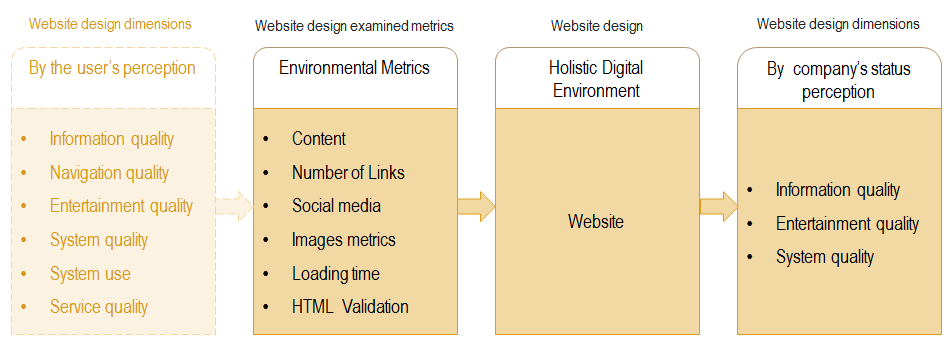
\includegraphics[scale=0.4]{../R/photos/001_model_framework.png} 
\end{center}
\end{figure}
Moreover the research framework that we will follow is to first identify the data that we will use, then gather them, following that we will proceed with the cleansing of the data and afterwards with their analysis in order to reach to the final stage of the results extraction.\\
In the chapter \textit{Literature Review} a retrospect of previous studies will take place and the thesis hypothesis will be presented. Moreover, in the chapter \textit{Data Gathering} an analytical description of the way we identified the data that we will collected and the way that they were collected from the website pages will be take place. Furthermore, in the next chapter called \textit{Data Analysis} the steps that were followed for the performance of the analytical part of the paper will be explained as well as the finding of this analysis. Finally in the \textit{Conclusion} chapter there will be a summarized version of the papers findings and its contribution to the already existing researches. The last chapter \textit{Further Research} will give some ideas of what the next steps should be regarding the current state of the field's research.
\newpage
\chapter{Literature Review }
The World Wide Web was created and developed in the United States of America and initially it was used from the government for educational and non commercial research institutions only. The first commercial use of the Web was not until 1993.\cite{key1} From then on there was an explosive growth that led to the existence of more than 200 million sites by 2005.\cite{key3} By now this number has been increased even more and it keeps growing daily. Nowadays it has become a part of the every day life of an average consumer. Taking into account this fact the research around the impact of the web pages into an organisation success is undoubtedly an interesting topic for examination.
\section{Empirical Studies}
For organizations the corporate website has emerged as one of the most important interfaces from where the consumers can infer a complete opinion of what the firm is standing for. Moreover there are many previous studies that have investigated the correlation of the website existence and the company's success. A content analysis of a website features was conducted in 1997\cite{key7} where the authors examined the companies of the Fortune 500 to see how many of those had web sites, in which industries did they belong to, whether or not where there any differences in the revenues regarding the existence of a site and the content of the pages. The findings of this research showed that even in 1997 the two thirds of the companies in the list had already set up their web pages regardless their industries. A research that was conducted two years later\cite{key10} again regarding the Fortune 500 sites showed that by then only 10 of the companies that where included in the 500 most successful ones in the U.S. continued to not have a web page. These findings show a very high correlation of successful companies with the use of web sites.\\
Furthermore in 2006 there has been a study that compared the use of websites in the top 1000 successful companies between two different countries\cite{key2} U.S. and Taiwan in order to understand the diversities in the web practices. This time the firms that were examined derived from the Fortune 1000 since the specific source was established in both countries. The results showed that the countries are in different stages regarding the maturity of the internet usage for consumer attraction. This shows that the best way to examine the upcoming trends is by concentrating in the most mature countries and to study the correlations there.\\
In the attempt to provide information regarding a vast number of different aspects of a website a great number of studies have been taken place.\\
Researchers thought that the internet and more specifically the Web is the best platform to attract more visitors and to reach new clients.\cite{key4} Based on this idea there have been conducted many studies that examined the best way to create websites. They believed that a consumer friendly design could add value to the users. This assumption was confirmed by previous studies that showed that a user interface that is perceived as very good is a vital factor in the retention rate of the visitors.\cite{key6} Of course in order to examine what exactly constitutes an excellent interface new studies had to take place.Wei-Shang Fan and Ming-Chun Tsai\cite{key5} in 2010 studied the relation between the internet customisation with the web design and the internet marketing strategy. This research showed that the web design quality can directly influence business performance.\\
The website design can be separated into six dimensions\cite{key9}:
\begin{enumerate}
\item \textbf{The information quality} : Researchers have suggested that the information that is include in a web site should be relevant to the purpose of the website\cite{key14, key16}, to provide an adding value to the consumer by being useful and educational\cite{key18} and last but not least to be easy to read and comprehensible.\cite{key19}
\item \textbf{The navigational quality} : This dimension is referring to the way the website has organized the information and how it has arranged them in terms of design, layout and sequence. The aspects that are included in this dimension and effect the ease with which the website can be navigated are the number and the effectiveness of hyper links and of course the overall structure of the information.\cite{key11,key20,key23,key24,key25}
\item \textbf{The entertainment quality} : The extent to which a website is visually appealing\cite{key19,key25} seems to be an indicator of how easy it is to use it. Another factor that makes the website easy to use is the use of graphics, multimedia and other interactive elements.\cite{key12}
\item \textbf{The system quality} : By referring to the system quality the technical properties of the website comes to mind. For example the ease with which the user can access the website. The access speed is characterized by how fast can the website download its pages and how fast it can display them.\cite{key19,key3,key22}
\item \textbf{The system use} : This dimension is also correlated with the technical properties of the website and is referring to the accessibility or the availability of the site.\cite{key24} The importance of accessibility can be observed from the fact that if the site is not available on a sustained basis, browsers would not be able to return to it.
\item \textbf{The service quality} : Finally the service quality dimension is referring to the capabilities and the option that the website is offering to their users.
\end{enumerate} 
Another important part of the Web usage from enterprises that should be taken into account is the use of the social media. One of the most representative definitions\cite{key27} of social media is the following: "\textit{a group of internet based applications that builds on the ideological and technological foundations of Web 2.0 and it allows the creation and exchange of users generated content}". This particular definition implies that the content of the social media is not consumed passively by the users but instead they react and even create their own content with their own views. This means that firms should actually participate in the social media fever if they want to reach out to their consumers and even to create new ones. Social media have become incredibly popular at a global level in the last few years. Facebook alone, a hallmark of social media has 1.86 billion active users per month as of the fourth quarter of 2016.\cite{key21} As active users are characterized those which have logged in to Facebook during the last 30 days. Also by the end of 2015 more than 50 million companies had already established their fan pages on Facebook.\cite{key26} In the following table the quarterly evolution from 2008 of the Facebook users shows us the gradually augmentation of Facebook users:
\begin{table}[H]
\centering
\caption{Facebook users by quarter}
\begin{center}
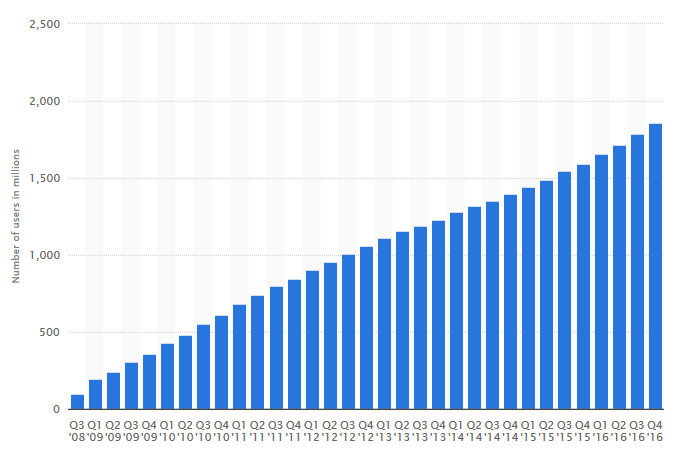
\includegraphics[scale=0.5]{../R/photos/facebook_q_users.png}   
\end{center}
\end{table}
Furthermore, due to this rapid evolution of the use of social media many different platforms have been created in the last few years. Some of the most popular ones, aside from Facebook, are:
\begin{itemize}
\item \textbf{Twitter} : As of the fourth quarter of 2016, the microblogging service 319 million active users per month.\cite{key28} From 2010 to 2013 the number of twitter users grew rapidly while from 2013 they continue to have an increasing course but at a smaller pace.
\item \textbf{Instagram} : As of December 2016, the mainly mobile photo sharing network had reached 600 million monthly active users.\cite{key29} Between December 2014 to December 2016 the number of active instagram users were doubled.
\item \textbf{Pinterest} : As of October 2016, the content sharing service has reached 150 million monthly active users.\cite{key47}
\item\textbf{Linkedin}: As of the third quarter of 2016, the business and employment-oriented social networking service had reached 467 million members.\cite{key31}
\item\textbf{Youtube} : As of January 2017,the 3rd most visited website in the world has reached over 1,3 billion active users.\cite{key32}
\end{itemize}
Our goal is to show how all those aforementioned metrics can be used to show the correlation of a website with the success of an enterprise. We can now develop our hypothesis. 

\section{Thesis hypothesis}
While there are quite a few previous researches that tried to correlated the success of a website with the overall success of a firm, most of the findings were derived from the perceptions of web users or web designers. Furthermore most of the variables at hand had to do with how those groups perceived the impact of them on their choices and not the actual prices of the variables that the company decided to use.\\
This paper extends beyond previous studies by devoting most effort on examining specific web site metrics that were deemed important from previous researches, not from the users perspective but from the actual metrics prices in relation to each enterprise's revenues.The questions that this study would try to answer are the following ones:
\begin{enumerate}
\item Do the revenues of a company correlate to specific metrics (or to some of the 6 dimensions of a website's design quality based on the user's perception) of the company's website?
\item Which of the metrics under examination are correlated (individually) the most with the revenues of each company of the Fortune 500 ones?
\item Which of the metrics under examination are correlated (in groups) the most with the revenues of each company of the Fortune 500 ones?
\end{enumerate}
\chapter{Data gathering}

\section{Data Source}\label{ds:f500}
The first step in order to contact this research is to find which companies will be examined. Since the purpose of this paper is to see if the website metrics that will be chosen are correlated with the success of a company it is a good idea to examine websites of some already successful firms and try to find out what they have in common. Moreover, we want to make this examination in a country that has already reach a certain maturity regarding the use of the internet for organizational purposes. Thus, we will examine the 500 companies that were ranked as the most successful ones from Fortune 500.\\
The Fortune 500 is an annual list compiled and published by Fortune magazine that ranks 500 of the largest United States corporations by total revenue for their respective fiscal years. The list includes public companies, along with privately held companies for which revenues are publicly available.\cite{key1, key2}\\
For the purposes of this paper,, we will use this list of companies and we will examine specific metrics of their websites in order to understand if there is a correlation between a firm's success and its on-line presence.\\
In order to gather the needed information from all the sites in the Fortune 500, we need to create an actual list of the names that are included in 2016 Fortune 500 ranking. In the variables collection section, the way that the list will be obtained will be explained in detailed. In the following table, the top 20 highest ranked enterprises of Fortune 500 during 2016 are available. The complete list by ranking is available in the Appendix A\ref{appA}.
\begin{table}[H]
\centering
\caption{Fortune 500 - 20 first companies}
\begin{tabular}{ll}
\hline
 \\ 1. Walmart 
&  2. Exxon Mobil 
\\  3. Apple 
& 4. Berkshire Hathaway 
\\  5. McKesson 
&  6. UnitedHealth Group 
\\ 7. CVS Health 
&  8. General Motors 
\\  9. Ford Motor 
& 10. AT\&T 
\\  11. General Electric 
&  12. AmerisourceBergen 
\\ 13. Verizon 
&  14. Chevron 
\\ 15. Costco 
& 16. Fannie Mae 
\\  17. Kroger 
&  18. Amazon.com 
\\ 19. Walgreens Boots Alliance 
&  20. HP 
 \\ \hline
\end{tabular}
\end{table}
Just to have a clearer idea of what do the companies under examination stands for we will analyse the first 20 ones so as to comprehend the industries and the type of firms that are included in the Fortune 500:
\begin{enumerate}
\item \textbf{Walmart }: is an American multinational retailing corporation that operates as a chain of hypermarkets, discount department stores, and grocery stores.
\item \textbf{Exxon Mobil } : is an American multinational oil and gas corporation.
\item \textbf{Apple } : is an American multinational technology company that designs, develops, and sells consumer electronics, computer software, and online services. The company's hardware products include the iPhone smart phone, the iPad tablet computer, the Mac personal computer, the iPod portable media player, the Apple smart watch, and the Apple TV digital media player. 
\item \textbf{Berkshire Hathaway } : is an American multinational conglomerate holding company. The company wholly owns GEICO, BNSF Railway, Lubrizol, Dairy Queen, Fruit of the Loom, Helzberg Diamonds, FlightSafety International, Pampered Chef, and NetJets, and also owns 43.63\% of the Kraft Heinz Company, an undisclosed percentage of Mars, Incorporated, and significant minority holdings in American Express, The Coca-Cola Company, Wells Fargo, IBM and Restaurant Brands International. 
\item \textbf{McKesson } : is an American company distributing pharmaceuticals at a retail sale level and providing health information technology, medical supplies, and care management tools.
\item \textbf{UnitedHealth Group } :  is an American managed health care company that offers products and services through two operating businesses, UnitedHealthcare and Optum, both subsidiaries of UnitedHealth Group. 
\item \textbf{CVS Health }:  is an American retail pharmacy and health care company. 
\item \textbf{General Motors }: is an American multinational corporation that designs, manufactures, markets, and distributes vehicles and vehicle parts, and sells financial services. 
\item \textbf{Ford Motor } :  is an American multinational automaker. The company sells automobiles and commercial vehicles under the Ford brand and most luxury cars under the Lincoln brand. Ford also owns Brazilian SUV manufacturer, Troller, and Australian performance car manufacturer FPV. 
\item \textbf{AT\& T } :  is an American multinational telecommunications conglomerate.
\item \textbf{General Electric }: is an American multinational conglomerate corporation. As of 2016, the company operates through the following segments: Power \& Water, Oil and Gas, Aviation, Healthcare, Transportation and Capital which cater to the needs of Financial services, Medical devices, Life Sciences, Pharmaceutical, Automotive, Software Development and Engineering industries.
\item \textbf{AmerisourceBergen } :  is an American drug wholesale company. They provide drug distribution and related services designed to reduce costs and improve patient outcomes, distribute a line of brand name and generic pharmaceuticals, over-the-counter (OTC) health care products and home health care supplies and equipment to a wide variety of health care providers located throughout the United States, including acute care hospitals and health systems, independent and chain retail pharmacies, mail-order facilities, physicians, clinics and other alternate site facilities, as well as skilled nursing and assisted living centers. They also provide pharmaceuticals and pharmacy services to long-term care, workers' compensation and specialty drug patients.
\item \textbf{Verizon } :  is a broadband telecommunications company and the largest U.S. wireless communications service provider.
\item \textbf{Chevron } :  is an American multinational energy corporation and active in more than 180 countries.
\item \textbf{Costco } :  is the largest American membership-only warehouse club that provides a wide selection of merchandise.
\item \textbf{Fannie Mae } : The Federal National Mortgage Association, commonly known as Fannie Mae, is a United States government-sponsored enterprise that provides financial products and services.
\item \textbf{Kroger } :  is an American retailing company. Kroger operates, either directly or through its subsidiaries, 2,778 supermarkets and multi-department stores. It maintains markets in 34 states, with store formats that include supermarkets, superstores, department stores, 786 convenience stores, and 326 jewelry stores.
\item \textbf{Amazon.com } :  is an American electronic commerce and cloud computing company.
\item \textbf{Walgreens Boots Alliance } :  is an American holding company that owns Walgreens, Boots and a number of pharmaceutical manufacturing, wholesale and distribution companies. 
\item \textbf{HP }: or Hewlett-Packard is an American multinational information technology company.
\end{enumerate}

It is obvious even from the first twenty companies that the firms that are included in the Fortune 500 list are from different industries and provide different products and services to the consumers. In previous studies the researchers tended to take into account the industry and divide the companies into groups. In this paper we will not create such a deviation since we want to see if there are some common variables across all the successful enterprises, regardless the industry they belong to, that can correlate with their success. This would mean that regardless of the specific needs that each industry should cover to its consumers there could be common needs to the website users that should be fulfilled prior to the specific industrial ones.
\newpage
\section{Metrics}
The next step is to identify the website metrics that will be examined. When a firm is referring to website metrics it usually means elements such as the number of page views, the number of visits, the number of unique visitors and also the geographical distributional of the users. These types of measurements are not available outside of the company, which is usually using a tool such as Google analytics\cite{key36} in order to track them. Since we cannot gather this kind of metrics we will have to examine metrics that are more related to how the site is structure and what exactly does the home page of each site includes. Those information can be retrieved from the HTML code of a company's site which is available for each internet user to see.\\
The two main categories in which we can divide the type of elements that we will retrieve from the website's HTML code are the following ones:
\begin{itemize}
\item \textbf{What we see:}\\
In the first category we are referring to metrics that can easily be conceived by the naked eye as well. For example the number of images that a website is using on its landing page and their dimensions. From the empirical studies that have taken place we saw that these variables have been examined as part of the entertainment quality measure. This means that previous studies examined the impact that the existence of images had on the users and not the relation that the actual number of images that are being used have with a company's revenue. In other words researchers have already examined the users perspective of what constitutes a visually pleasant website but not what do the firms decide to actually implement on their websites.
\item \textbf{What lays behind of what we see:}\\
The second category is not so obvious and it includes information that usually is visible only to the web developer or the creator of the page. The information can only be taken by the HTML code and not with the naked eye. For instance we can see the type an image, an information not visible with the naked eye.
\end{itemize}
Now that we have a first understanding of the two main categories that the metrics can be divided in, we can see in detail the metrics that will be examined in this paper:
\subsection{Loading time}\label{M:Loading time}
One aspect of a website that is crucial is the time it takes for it to load. Nowadays that the internet speed is going higher and higher most people do not have the patient to wait for a page to load. Several user experience studies evaluate how page load times impact user satisfaction. The ill effects of slow websites are well documented. Recent surveys suggest that 49\% of users will abandon a site or even switch to a competitor after experiencing performance issues. This highlights the importance of including this measurement to the study and determine it's relation with the company's status in terms of revenues.
\subsection{Number of links}\label{M:Number of links}
The overwhelming information that is available on line can render a user incapable of finding the piece of information he is looking for. Many internet users tend to browse across different sites searching for a particular information that they cannot remember where they have found it before. Considering this tendency firms should create hyper links that will make the navigation into the site easier for the user but will also give him the opportunity to grasp the highest level of information that he can. This translates to the existences of internal but also external hyper links. An internal link can direct the user to another page of the same site while an external link can lead the user to another site.\\
The internal links are responsible mainly for the ease of navigation on the website. The better their structure the easier it gets for the user to find what he is looking for. The external links are mainly responsible for the quality of available information. Based on the industry that a firm belongs to, it has to provide the users with information that can be relevant not only for the specific company but also for the whole industry. Sometimes those information are not available or cannot be available in the enterprise site so the firm should be proactive and create hyper links that will lead the user to the information that he is looking for regardless if this can be found on their site or not. With this approach the user gets a feeling of satisfaction that is connected with the firm's website that helped him find the information he needed.\\
For the purpose of this paper since it is not so clear which type of links are more important to a user we will examine both the internal and the external links and moreover the total links of a website to see which of those three indicators is correlated the most with a firm's success.
\subsection{Social media}\label{M:Social media}
Our era is marked by the social media wave that has changed our lifestyle and our daily habits. So it would be considered an oversight if we didn't take into consideration the number of social media that the company chooses to participate in. Even though they can also be considered as external links of the website we will examine them separately in order to see if any particular social medium effects the company's revenues. Since there is an ongoing debate on whether social media should be used from firms to attract customers or if their use should be only for connecting people with each other and not brands the results of this paper would give a perspective of what is really happening in terms of numbers and not from the users perspective.
\subsection{Number, format and pixels of site's images}\label{M:N,T,S Imgs}
Since the site is the first thing that a user will see on line regarding a company and there is a famous quote that says that \textit{"First impressions counts"} we should also examine how the companies decide to visualize their landing page. In other words to see how many images they include in it. An great way to see that is to count the number of pixels that appear in the web page under examination.The purpose is to examine if the pixels diversities between the examined websites are actually correlated to how they are doing success wise.\\
Moreover an information a little more complicated for a simple user to understand, but which  plays a very important role in many cases is the type of the image. For example some websites are using specific formats of images or banners that are not compatible with all the browsers, leading the user to see some break points on the website and even stop visiting it. Based on those facts we will examine the most commonly known type of images and see in which degree they are being used by the companies under examination and whether or not there is a correlation with the revenues.
\subsection{Content} \label{M:Content}
They say a picture worth a thousand words but that is not enough in our case. After exploring the number, sizes and type of pictures that a website is using we should also explore the number of words it is using to accompany the images and complete the outcome that a user will come across. The metrics we will use will be two. The first one will be the total words that are being used on the landing page and the other one will be the total unique words that are being used. When we are referring to unique words we mean words that are not so commonly use such as "a" or "and" and they give an air of individuality to the text. By using this metric we would try to see if the words that are being used are just as important as the actual content and if the words can make a difference.\\
Furthermore we should also take into consideration how comprehending is the text used on the websites for the users. This information can be obtained by calculating the readability index of the website and also the number of sentences that exists in a page (a metric that comes to complete the previous ones).How the readability index is being calculating will be furthered explained in the variables collection section.
\subsection{HTML Validation} \label{M:HTML Validation} Moreover we will have to check the quality of the HTML code behind the website we are seeing. Are there any mistakes in the code for example any brackets that opened and never closed or any links that do not work. We will examine again two different metrics here the number of errors and the number of warnings. The warning are parts of the code that even though they work at the time there is a good chance to malfunction if any changes or addition are to be made to the HTML code. 
\newpage
\section{Python Language}
After explaining the reasons that we decide to explore the variables/ metrics that were mentioned in the previous section we should now see how we are going to obtain all these information.\\
Since the needed information can be subtract from the HTML code of a company's website we should use a programming language in order to download the HTML pages and then to extract the specific metrics we want to examine.\\
For the purposes of this paper,, the programming language that will be used for downloading the website's HTML code and then extract from them the metrics is Python. More specifically the version of Python that will be used is the 2.7 one.\cite{key43}\\
Python is a widely used high-level programming language used for general-purpose programming, created by Guido van Rossum and first released in 1991. An interpreted language, Python has a design philosophy which emphasizes code readability (notably using white space indentation to delimit code blocks rather than curly braces or keywords), and a syntax which allows programmers to express concepts in fewer lines of code than possible in languages such as C++ or Java. \\
The language provides constructs intended to enable writing clear programs on both a small and large scale. Furthermore the way that Python allows a user to programming is common to all users which gives this language a leverage as a program build in Python can be easily understood by another user without any difficulty.\\
The environment that is going to be used is from the Anaconda package which is a free open source distribution of the Python and R programming languages for large-scale data processing, predictive analytics, and scientific computing, that aims to simplify package management and deployment. To be more precise from this package we are going to use the Jupyter Notebook. All the scripts that were created in the Jupyter Notebook are available in the Appendix.\ref{appP}
\newpage
\section{Variables collection}
In order to gather all the needed metrics we had to create a variety of small scripts so as to collect them. In this section we will present in detail the procedures that were used in order to create the scripts and extract the information that later will help us contact the analysis of the relationship between those metrics and the company's status. 
\subsection{Companies ranking, names and url}
For starters we need to create a list of the names, the ranking and the URL of the sites that we will later download and extract the necessary info from them. So as it was mentioned in the previous section\ref{ds:f500} the first step that needs to be done is to download and gather those information into a data frame\footnote{a table in Python environment with rows and columns} so as to be able to use them later on.\\
The easiest way to obtain this list is by retrieving it from an already existing list that has been created in an article on line.\cite{key33}. The way to keep only those three information as different variables is by separating from the HTML code of this page the needed elements.\\\\
\textbf{Step 1} : The first step is to create three empty lists where we will include the information we are going to extract. The first list will contain the rank of each site as a number, the second one will contain the name of the company as a text and the 3rd one will contain the actual link of the company's site again as a text and without the http:// in the beginning.\ref{p1}\\\\
\textbf{Step 2} : The second step is to upload some libraries that will help us create this function but also the rest ones that are going to follow.\ref{p2}\\\\
\textbf{Step 3} : Finally the third step is to create the function that will firstly download the HTML code of the url at hand, secondly keep only the part of the code that we need to examine and thirdly save this part into the empty lists we created above. This function is called websites and takes as variable to work only the url of the site we need to examine.\ref{p3}. More specifically the methodology we followed to create the following function are the following:
\begin{enumerate}
\item We create a fake browser that we are going to use in order to open the page and downloaded. The reason we do that is that many sites do not allow us to download their page because they are afraid of stealing important information. Since we are not using any private information we use this method to avoid issues while trying to open the HTML page at hand. 
\item We open the url and we read it while saving it in the variable "myHTML".
\item With the help of the Beautiful Soup library\footnote{Beautiful Soup is a Python library for pulling data out of HTML and XML files} we read the page as a lxml file and then for each row of this file we are looking for the "td" parts of the code where the information we want are included.
\item Since we need the names and the urls of all the 500 sites we created a loop from 0 to 500 where for each i we try to isolate the part of the code that contains the information that we want. Moreover even though it seems that with this loop we calculate 501 numbers since in Python the second bracket is always open we actually count from zero to 499.
\item We use reg expressions\footnote{A regular expression is a special sequence of characters that helps you match or find other strings or sets of strings, using a specialized syntax held in a pattern.} in order to state precisely what part of the already selected code we want to keep.
\item We insert with a specific order the names, the ranking and the url to the corresponding lists and finally we create a text that will appear when the function is completed. Here we have also calculated the time that this function took to be completed and we will appear it as well along with the text.
\end{enumerate}
\subsection{URL validation}
Now that we have saved in the three lists the names, the ranking and the URL of the companies that we are going to examine we first have to check whether or not those URL are valid in order to proceed with the download of the HTML code behind the initial web page of each one of those companies.\\\\
\textbf{Step 1} : We first have to install the validators package in python so as to proceed with the validation of the url. In the command prompt window that opens when you open the Jupyter Notebook you have to write: "pip install validators" and then press enter in order for the package to be installed. This specific package currently supports python versions 2.7, 3.3, 3.4, 3.5 and PyPy.\footnote{https://validators.readthedocs.io/en/latest} The function that we are going to use from this package is called validators.url. This functions returns True if the url at hand is a valid url or False if it is not.\\\\
\textbf{Step 2} : Next we created a loop that will run as many time as the length of the list that we created in the previous section.\\\\
\textbf{Step 3} : During this loop we create a string variable where we use the URL that we have saved in the list, one at each time, and we add the "http://" prefix.\\\\
\textbf{Step 4} : Now that we have create the correct way that a url is supposed to be written we will use the function of the validators package and we will create an if function that will check if the answer to a site is different from True and if it is it would add a unit in the variable nv so as to know at the end how many sites did not had valid URL.\\\\
\textbf{Step 5} : Finally we ask from the programme to print the final result so as to know how many URL are not valid. The code that was created for this procedure is available in the Appendix.\ref{p4}\\
In our case all the URL where valid so we are eligible to proceed at the next part of the code.
\subsection{Download sites HTML code}
After checking the validity of the URL that we have saved in the list the next step is to download the actual HTML code of the initial pages of each one of the 500 websites we want to examine.\\\\
\textbf{Step 1} : As we did in the section 2.4.1 we have to create a fake browser so as the to be able to download the HTML code without contacting any problems. In our case we created a Mozilla browser.\\\\
\textbf{Step 2} : In order for the url to be opened we must first bring it to the correct form. Initially we create again a loop and for each loop we will examine a specific url. We first replace some symbols on the string that will not be recognized if we try to open the url in this form and then we add the "http://" in the begging of each url.\\ \\
\textbf{Step 3} : Before starting downloading we create some rules for some exceptions. For example the sites 71 (Best Bay),119 (Arrow Electronics) and 465 (St. Jude Medical) in ranking create problem when we tried to download them and the code is stop working. So in order to avoid such incidents we created an exception and the python code will not even try to download these sites and in their position in the new list of the HTML pages that we will create a zero will be saved.The same thing would happen if an exception is thrown in the function if that we are creating. In any other case we will open the site and save this action in the variable response2.\\\\
\textbf{Step 4} : After saving the action we will use the command read and we will save the HTML code which is essentially a long piece of text and then we will save this "text" in the list.\\\\
\textbf{Step 5} : Finally we will wait for 2 seconds in order for the browser not to be suspicious from the extreme speed that we are going to open the next page. In that way we avoid having any crushing incidents on the code.\\\\
\textbf{Step 6} : After completing this procedure for all the site we will have a list that in each position the HTML code will be held as a very large text. Except from the sites that were not able to be opened.\\
The code that was created for this procedure is available in the Appendix.\ref{p5}
\subsection{Not downloadable pages}
As we explained in the previous section there are some pages that were not able to be downloaded. In order to know which are those pages and more specifically which companies sites will not be available for further exploration we created this part of the code that creates a list of the names of those companies.\\
In the previous code we used a zero in each position that we weren't able to download the site. Here we will use this information in order to gather in a new list only the parts of the list that did get a zero.\\
Here we created a small function that is called "not downloadables". In the first part of the code we create the function and in the second part we run the function for our lists. Finally we create a data frame with the results so as to be more easy on the eyes.\\
The code that was created is available in the Appendix.\ref{p6}
In the following table we can see the sites that were not downloaded: 
\begin{table}[H]
\centering
\caption{Not downloadable sites}
\begin{tabular}{ll}
\hline
 &  \\ 
16. Fannie Mae 
& 63. HCA Holdings \\
71. Best Buy
& 91. Nike \\
98. Tesoro 
& 119. Arrow Electronics\\
136. AutoNation
& 142. Southwest Airlines \\
162. Southern 
& 165. American Electric Power\\
196. Office Depot 
& 217. PBF Energy \\
229. Consolidated Edison
& 240. Toys “R” Us \\
243. Dominion Resources 
& 276. Global Partners\\
307. PayPal Holdings 
& 327. News Corp. \\
364. Williams 
& 415. Tractor Supply\\ 
442. Old Republic International 
& 465. St. Jude Medical \\
\hline
\end{tabular}
\end{table}
\subsection{Content}\label{content}
Now that we have downloaded the HTML code we should start extracting some of the variables we are going to use for the analysis in the next chapter.\\\\
\textbf{Step 1} : The first thing we are going to check is how easy it is for a user to read the content of each site. In order to check this performance indicator we will need to gather 4 variables:
\begin{enumerate}
\item Number of Words
\item Number of Unique Words
\item Number of Sentences
\item Flesch score
\end{enumerate}
The three first are quite clear. The number of words are the total words that appear in the texts that the user is seeing in a website. The number of unique words are the words that are not very common and can attract the readers attention or even make it harder for him to comprehend the text. The number of sentences is related to those variables as we can understand from this is comparison to the number of total words how big or short is the sentence and as a conclusion how easy or not is the complete text.\\
Finally regarding the forth variable the flesh score is referring to the Flesh reading ease test score.In the Flesch reading-ease test, higher scores indicate material that is easier to read; lower numbers mark passages that are more difficult to read. The formula for the Flesch reading-ease score (FRES) test is:\\ \\
$206.835 - 1.015 (total words/total sentences) - 84.6 (total syllables/total words)$\\
\\
We will calculate the flesh reading test and the other three aforementioned variables with the help of an on-line readability test tool.\cite{key34} This site calculates and return all these results that we need. The way to implement them in a new data frame to our python code is by dividing the HTML code, behind the page with the results for each site, and keeping only the actual numbers and sizes that we seek. \\\\
\textbf{Step 2} : We create four lists where we will save the variables that we are looking for. Then we start a loop for the 500 sites where in each loop we change the value of the 3 main variables the sites that contain the HTML code the url that contain the url of the company at hand each time and the url check where we save the part of the web address that remains the same while doing the on line check and we add at the end the url of the site we want to check. Also we open the browser as we have done in previous scripts as well.\\\\
\textbf{Step 3} : Then we create an if part where we check that the variable site is not zero and that we will not examine the site 108 (Tech Data) as the code seems to have a problem in that case. In this check we put on the respective sites n/a values so as to be clear that we did not retrieve these info for them.\\\\
\textbf{Step 4} : We open the browser link and we check whether or not we drop to any exception in which case we also put n/a values in the respective companies.\\\\
\textbf{Step 5} : We read the link and after checking that it is not empty (this we  can check by comparing it with an empty list that we have created for this use) we use the Beautiful soup library to extract the part of the code that we need.\\\\
\textbf{Step 6} : After taking a look at the HTML code of the pages we find out that the parts that we need are between the following brackets <tr>...</tr> so we will extract each such bracket from the code and save them in a list. By checking the list we found which numbers of the list items we want and we saved them in the variables we have created. Always of course checking first that the specific prices exist or in any other way we again put n/a.\\\\
\textbf{Step 7} : Now that we have the for key indicators that we will use later on the analysis we should also create a more easily comprehend variable that is related to the flesh measure variable we just created. The numbers that each site gathered mean different things. So we will try to create a correlation and build a variable called readability that will say in text how easily read or not a site is. The score can be interpreted by the following logic:
\begin{itemize}
\item Flesch measure $<$ 30 : Very Confusing
\item Flesch measure $>$ 30 : Difficult
\item Flesch measure $>$ 50 : Fairly Difficult
\item Flesch measure $>$ 60 : Standard
\item Flesch measure $>$ 70 : Fairly Easy
\item Flesch measure $>$ 80 : Easy
\item Flesch measure $>$ 90 : Very Easy
\end{itemize}
\textbf{Step 8} : We created a function that creates a new list where the flesh measure variable is being saved as the above descriptions based on the scores each of the site achieved.\\\\
\textbf{Step 9} : Now that we have all the needed information in lists we should combine them by creating one data frame with the use of the variable company name again in order to have a common key so as to merge all the data frames that we will create in the end.\\
The code that was created is available in the Appendix.\ref{p7}\ref{p8}

\subsection{HTML Validation}
After downloading and saving in data frames the first batch of metrics that we will need for the analysis we should also check the quality of the HTML code.\\
Most pages on the World Wide Web are written in computer languages (such as HTML). One of the advantages of writing in a computer language is that it allows the developer to structure text, add multimedia content, and specify what appearance, or style, the result should have based on his needs.\\
As every speaking language,so the computer languages do have their own grammar, vocabulary and syntax too. Each document that is written in these computer languages is supposed to follow these rules in order to consider it well structure and written.\\
However, just as texts in a natural language can include spelling or grammar errors, documents using computer languages may (for various reasons) not be following these rules as well.\\
The process of verifying whether or not a document actually follows the rules for the language it uses is called validation, and the tool used for that is a validator. A document that passes this process with success is called valid.\\
With these concepts in mind, we can define "validation" as the process of checking a web document against the grammar (generally a DTD\footnote{DTT: Document Type definition}) it claims to be using.\\
For the purposes of this paper, we will use an on-line validator site called W3C\cite{key50} which will help as see how many errors and warnings does each site have. \\\\
\textbf{Step 1} : Initially we create the empty lists in which we will save the variables we will extract that will give as a clear glance on how many errors does each page has, how many warnings, how many pages weren't recognized as documents and how many pages did open during the process.\\\\
\textbf{Step 2} : The next step is to create a function that will do a similar job as the script we used to extract the previous variables. Initially we locate the part of the url that remains the same when the check is completed and we see the part that does change where the name of the url we want to examine should go. In order for the code to recognize that we save the result in a variable that in the end is a new url that when we open it, it will show as the page of the results for each site in each loop that we are examining.\\\\
\textbf{Step 3} : One difference in this script is that now the part of the code that we need is not between $<tr>..</tr>$ but between $<div>...</div>$ parts of the code. So we follow the same procedure as before and we locate in the list of all the divs that we create with the help of the Beatuful soup package the parts that gives us the information we want to keep.\\\\
\textbf{Step 4} : One other difference is that here after the procedure ends we have counted the actual time we needed to complete this procedure. Then next step is to run the function we created.\\\\
\textbf{Step 5} : Finally we save the lists that we created in a new data frame where the common column remains the name of the company as it already is in the previous dataframes we have created.\\
The code that was created is available in the Appendix.\ref{p9}
\subsection{Social media}
One other group of variables that we should include in our analysis is the social media that each company choose to use. Since this era is being characterized from the massive use of social media we can't help but wonder if some of them could actually play a crucial role in a business success.\\
The way we are going to see which social media does a company use is quite simple. We will create a list of the name of each of the  six most well known social media with the suffix ".com" and then we will check if the expression appears in the HTML code of each company. If an expression does exists that means that the specific company does indeed uses this specific social media and as so it appears a respective link in it's home page so as the user to have the opportunity to subscribe in it.\\
The procedure we will use is similar to the previous ones.\\\\
\textbf{Step 1} : Firstly we create the lists for the social media that we want to examine. More specifically the social media we will search for are the following:
\begin{itemize}
\item\textbf{Facebook}: a social media that lets you upload images, thoughts, songs and lets you interact with your friends
\item\textbf{Twitter}: an on-line news and social networking service where users post and interact with messages, "tweets," restricted to 140 characters
\item\textbf{Pinterest}: an internet photo sharing and publishing service that allows users to "Pin" pictures they like and upload their own recommendations to their "pinboards".
\item\textbf{YouTube}: a free video sharing website that lets people upload, view, and share videos. 
\item\textbf{Instagram}: an online photo and video sharing social networking service. It allows users to take pictures and videos, apply digital filters to them and share them to their followers. 
\item\textbf{Linkedin}: a social networking website for people in professional jobs. Users can make connections with other people they have worked with, post their work experience and skills, look for jobs, and look for workers.
\end{itemize}
\textbf{Step 2} : The next step is to create a function that first creates the lists with the 6 elements we would search on each HTML code. \\\\
\textbf{Step 3} : Then after checking that the HTML code for each specific site has been downloaded properly (in other words is not equal to zero) we search in a loop for each of the social media at hand if it exists in the HTML code. If it exists we put True in the respective list.After completing this procedure we export also the time we did to run the function.\\\\
\textbf{Step 4} : Now that we have the function ready we run it and afterwards we again save the results in a new data frame.\\
The code that was created is available in the Appendix.\ref{p10}

\subsection{Links - Internal and External}
The navigation inside a website is extremely important as we mentioned in the literature review and highly correlated to the number of hyper links that are included in it. Thus, the next step is to see how many internal, external and finally total links each HTML code has. The links show in how many other pages does this home page leads to. If the links are external that means as we said in the Metrics section that they lead in a page that is not of this website. While the internal links lead to other pages in the same website.\\
By extracting this information we want to see if it is important for the user to have the ability to browse in various pages inside the site from the home page and also if it plays any role the use of external links that give the user the opportunity to be transferred in another site that is relative of course with the one he is looking in.\\\\
\textbf{Step 1} : A great way to spot the links in an HTML code is the prefix that they all use which is "href". So the first step (after creating the initial lists of course and the loop we do in each script) is to locate how many times does the expression "href" appears in the code. The result of this search will give us the total links of the site.\\\\
\textbf{Step 2} : Next step is to separate somehow the internal and the external ones. An easy way to do that is to find all the "href" references that are followed by "="https: ". By locating specifically those expressions we have located all the external links because unlike the internal links that do not need to be written in this form the external links since they lead to other sites they should always begin with this expression.\\\\
\textbf{Step 3} : Now that we have the total links and the external links as well we can easily find the internal links with a simple subtraction:
\begin{center}
\textit{total links - external links = internal links}
\end{center}
Finally we put the results in the respective lists for each site and we export the time we did to run the script.\\\\
\textbf{Step 4} : Now that the function is completed we run it and then we create a data frame as we have done in the previous scripts as well.\\
The code that was created is available in the Appendix.\ref{p11}

\subsection{Loading time}
One very important factor as we mentioned before\ref{M:Loading time} is the time that the site does to be loaded and with this part of the code we will count exactly that.\\
We have already counted in previous scripts the time they did to be completed. In a similar logic we will count the time it does for the browser create after opening the url to read it.\\\\
\textbf{Step 1} : The procedure is the same, firstly we create the empty list where we will save the time it does to open for each site. \\\\
\textbf{Step 2} : Then we create the function and we create the loop for the 500 sites. In case of an exception we put "n/a" in the respective list position or if the site is the number 119(Arrow Electronics) or 465(St. Jude Medical)\footnote{or 118/464 in the loop's numbering since it start from zero} which create a problem in the code and we continue. In the end of the function we appear a text that lets us know that the process has been completed.\\\\
\textbf{Step 3} : Next step is to run the function and finally create a data frame with the results.\\
The code that was created is available in the Appendix.\ref{p12}

\subsection{Number, format and pixels of site's images}
We reach to the final group of variables that we are going to examine regarding the home pages of the websites of the 500 companies that ranked first in Fortune 500. This group has to do with the images of each site. We can divide the information that we want to extract into 3 major categories:
\begin{enumerate}
\item Type of images
\item Number of images
\item Different image sizes
\end{enumerate}
\subsubsection{Images formats}
There are many different types of images that can be used in a site. Here we will try to see between the most common types which ones are the most preferable from the sites and later on in the analysis to see if this has any correlation to their success. The type of images that we will examine are the following ones:
\begin{itemize}
\item \textbf{PNG}: Portable Network Graphics (PNG) is a raster graphics file format that supports lossless data compression\footnote{Lossless compression is a class of data compression algorithms that allows the original data to be perfectly reconstructed from the compressed data}.
\item \textbf{BMP}: Bitmap (BMP) is a raster graphics image file format used to store bitmap digital images, independently of the display device (such as a graphics adapter), especially on Microsoft Windows and OS operating systems.
\item \textbf{DIB}: Device-Independent Bitmap (DIB) is a graphics file format used by Windows. DIB files are bitmapped graphics that represent color formats. Similar to BMP format, except they have a different header. DIB files can be opened and edited in most image editing programs.
\item \textbf{JPEG/JPG/JPE}: The term (JPEG) is an acronym for the Joint Photographic Experts Group, which created the standard method of lossy compression for digital images, particularly for those images produced by digital photography. The degree of compression can be adjusted, allowing a selectable trade-off between storage size and image quality. JPEG typically achieves 10:1 compression with little perceptible loss in image quality.
\item \textbf{GIF}: The Graphics Interchange Format (GIF) is a bitmap image format that supports up to 8 bits per pixel for each image, allowing a single image to reference its own palette of up to 256 different colors chosen from the 24-bit RGB color space. It also supports animations and allows a separate palette of up to 256 colors for each frame. These palette limitations make the GIF format less suitable for reproducing color photographs and other images with continuous color, but it is well-suited for simpler images such as graphics or logos with solid areas of color.
\item \textbf{TIFF/TIF}:Tagged Image File Format (TIFF or TIF) is a computer file format for storing raster graphics images, popular among graphic artists, the publishing industry and photographers. The TIFF format is widely supported by image-manipulation applications, by publishing and page layout applications, and by scanning, faxing, word processing, optical character recognition and other applications.
\end{itemize}
As we can see some of the type of images have more than one ways that can appear so in order to be precise we will examine all nine different endings. The procedure we will follow is the same one. \\\\
\textbf{Step 1} : Initially we create the lists we will use then we create the function and the loop for the 500 sites.\\\\
\textbf{Step 2} :  For each site we check if the HTML code is not empty and then we search for all the endings that exists in each site and we save in the lists the number of times the ending appeared so as to know how many such images the site has.
\subsubsection{Number of images}
\textbf{Step 3} : The total number of images is the sum of all the different types of images and the number of each of those in a site. So in order to catch to birds with one stone we create a variable in the same function where in each loop for each different type of image it adds them in this variable so as to have the total images in the end.\\\\
\textbf{Step 4} : In the end of the function we export the time the function did to run again. The next step is to run the function and finally create the data frame with the variables we created.\\
The code that was created is available in the Appendix.\ref{p13}

\subsubsection{Pixels of images}\label{dif_img_s} 
Aside from the number of images and the types that are being used another important factor is the pixels of an image. In digital imaging, a pixel, or picture element is a physical point in a raster image, or the smallest addressable element in an all points addressable display device. So it is the smallest controllable element of a picture represented on the screen. The more pixels used to represent an image, the closer the result can resemble the original. In the following code we will find the array of the pixels of all the images of each site and then we will sum them up to a final result that will be comparable across different web pages. \\\\
\textbf{Step 1}: The first step is import the libraries that we are going to use which are the numphy library and the urllib one. \\\\
\textbf{Step 2}: Next we open the url of the website we want to examine.\\\\
\textbf{Step 3}: Then we use the numphy library to create a numphy array that will contain all the pixels of all the images in the web page under examination. \\\\
\textbf{Step 4}: Now that we have all the pixels we create a loop and we add them up in order to end up with one total number of the pixels that are containing in the web page at hand..\\\\
\textbf{Step 5}: We run the function.\\\\
\textbf{Step 6}: We create the data frame with the informations that we gathered.\\\\
The codes that was created is available in the Appendix.\ref{p14}                

\subsection{Fortune 500 - Metrics download}
Just in order to have some metrics that will depict the status of the companies, we will also download some metrics from the Fortune 500 sites for each company.\cite{key35} In order to achieve that we should open the pages for each one of the sites separately. Since there is a pattern in the way the pages are named it shouldn't be difficult.\\
\textbf{Step 1}: Firstly we should create the pattern with which we will download the pages. By running the code we can see that the names of each company are not written exactly as we have saved them.\\\\
\textbf{Step 2}: So the second step we need to do is to alter the names that are not similar in order for the next functions to run.\\\\
\textbf{Step 3}: Now that we have the correct names we can download the HTML code of each one of the fortune 500 companies pages from the fortune 500 site so as to extract the information we need. Again here we follow the same steps. Firstly we create an initial list and then a function and a loop for the 500 sites. And for each loop turn we download and save the HTML code behind the fortune 500 page for the site at hand. Finally we run the function.\\\\
\textbf{Step 4}: Now that we have saved the HTML codes we are going to extract some information that we need from them. In order to do that initially we have to create the variables we will need.\\\\
\textbf{Step 5}: Now that we have the initial variable we are going to create a function in order to extract the specific parts we need. More precisely we are going to download the following information:
\begin{itemize}
\item Revenues in dollars
\item Assets in dollars
\item Total Stockholder Equity in dollars
\item Market Value in dollars
\item Profit in dollars
\item Profit as \% of Revenues
\end{itemize}
For each loop we use the library Beautiful soup to find all the parts between $<tbody>...</tbody>$ and we locate in which of the parts do the elements we want to extract lies on.\\\\
\textbf{Step 6}: After locating them we find in this specific part all the parts that are between $<td>...</td>$. Then we locate in those new parts where each of the information we need is and with the help of the regular expressions\footnote{A regular expression is  a sequence of characters that define a search pattern. Usually this pattern is then used by string searching algorithms for "find" or "find and replace" operations on strings} we keep only the numbers of each part.\\\\\textbf{Step 7}: We do that separately for each one of the five variables we want to create and finally we print that the function is completed.\\\\
\textbf{Step 8}: Next we run the function\\\\
\textbf{Step 9}: Finally we create the data frame with the elements we extracted.\\
The codes that was created is available in the Appendix.\ref{p18}

\subsection{Merge data-frames and extract final csv file}
The final step in order to conclude the section with the downloading and gathering of the data is to create a final data frame which will include all the information gathered and then create a csv file that will be used for the further analysis that will be take place with the use of the program language R.\\
In order to do that we merge the data frames we created by two using the company name as key and then we repeat the merging procedure until we end up with only one data frame that will include all the others.
Finally we create the csv file that we will use in the analysis in R in the next chapter. The code that was created is available in the Appendix.\ref{p23}
 
\chapter{Data Analysis}
By concluding the gathering of all the information needed the next step is to proceed to their analysis. For the purposes of this assignment we will use the programming language R to perform this analysis.\cite{key1}\\
In this section we will present the steps that we followed to contact this analysis and also we will explain elaborately the findings. The analysis that we are going to perform will be explained by the following order as it was performed:
\begin{enumerate}
\item Data cleansing
\item Variable analysis and correlation
\begin{enumerate}
\item Fortune variables analysis and correlation
\item Social media analysis and correlation
\item Links analysis and correlations
\item Words analysis and correlation
\item HTML validation variables analysis and correlation
\item Image types, number and pixels analysis and correlation
\end{enumerate}
\item Logistic Regression
\end{enumerate}
\section{R Language}
R is a programming language and software environment for statistical computing and graphics supported by the R Foundation for Statistical Computing. The R language is widely used among statisticians and data miners for developing statistical software and data analysis.\\ 
Furthermore R is freely available under the GNU General Public License, and pre-compiled binary versions are provided for various operating systems. While R has a command line interface, there are several graphical front-ends available.\\
For the purpose of this paper we will use the R-Studio which  is a free and open-source integrated development environment (IDE) for R.
\section{Data cleansing}
Before we will be able to begin the analysis we should first check the data that we have gathered.\\
The first step is to upload in the R environment the csv file we have created and see how many variables and observations we have. The data have 500 observations as it was expected since we will examine 500 companies and 38 variables.\\
The next step is to change the decimal point in the variables we gathered from the Fortune 500 site in order to be read correctly from R.\\
Moreover, we should make all the variables numeric in order to be more easy to compare them. The only variable that we keep as factor is the Readability one since we made it on purpose like that so as to have a clear view of what the flesch test results really mean.\\
Moreover we should omit all the variables and observations that contain na's from this analysis so as for the results to have a point.\\
The next step is to rename some variables in order to have a better and clearer understanding of what they represent. For example a variable named X that was added when we extracted the csv from Python represents the actual ranking of each company, an information that will prove to be very useful later on. So it will be a good idea to rename this variable to Ranking.\\
Some of the variables while they were important during the python scripts they do not actually play any important role in this analysis and we should remove them from the beginning of the analysis. For instance the company's url was an important variable while we ran the python scripts but since there are unique for each site they cannot give us any useful information for the analysis we want to perform.\\
Another important step before going on with the analysis is to upload the libraries that we are going to use further along. More specifically we will upload the following libraries for starters:
\begin{itemize}
\item \textbf{ggplot2}: The ggplot2 package, created by Hadley Wickham, offers a powerful graphics language for creating elegant and complex plots.
\item \textbf{reshape2}: The reshape2 is an R package written by Hadley Wickham that makes it easy to transform data between wide and long formats.
\item \textbf{DAAG}:This package is called Data Analysis and Graphics Data and Functions and it consists of data sets and functions.
\end{itemize}
Finally the number of the observations and the variables that we are going to use in the analysis have been change to the following ones:
\begin{table}[H]
\centering
\caption{Dataset initial and after cleansing}
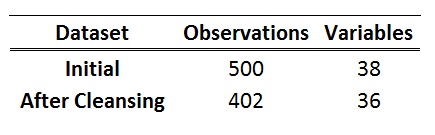
\includegraphics[scale=0.6]{../R/photos/002_dataset.PNG} 
\end{table}
The script we used to perform all the above steps could be found in the Appendix.\ref{r1}
\section{Fortune variables analysis}
Now that the variables are cleansed we can perform the first step of the analysis which is the analysis of the variables so as to have a first look of how they are distributed and how they are correlated to each other. In order to proceed with this analysis we have to separate the variables into same groups as we did when we downloaded them and examine them together to see if some of those prices are correlated.\\
The procedure is to first take a look of each variable of each group separately and then in relation to the variable of the fortune 500 that we will choose and then see the correlation of all the variables in each group with the fortune 500 variables.\\
In statistics there are two main types of regressions the linear and the logistic regression. The linear regression is an approach for modelling the relationship between a scalar dependent variable y and one or more explanatory variables (or independent variables) denoted X. The case of one explanatory variable is called simple linear regression. For more than one explanatory variable, the process is called multiple linear regression.\\
The logistic regression, or logit regression, is a regression model where the dependent variable (DV) is categorical.Cases where the dependent variable has more than two outcome categories may be analysed in multinomial logistic regression, or, if the multiple categories are ordered, in ordinal logistic regression.\\
Moreover when a regression analysis is being done with one independent variable and one dependent one we call it simple regression analysis. While when the regression analysis is being done with multiple independent variables and one dependent variable we call this analysis multiple regression analysis.\\
In this chapter we will perform both of these analyses in order to get a full picture of the correlations between the variables of the websites and the variables of the fortune 500 we have collected.\\
The first step is to determine the variable with which we will compare all the other ones. Obviously this variable will be one of the metrics we downloaded from the fortune 500 site so as to have an actual variable that shows the status of the company and compare the rest of the variables with it.\\
First of all we should see the summary of the variables we have downloaded in order to have an initial idea of the prices we are going to see. In the below table we can see the min price, the max price, the mean and the medium of each one of the fortune 500 variables:
\begin{table}[H]
\centering
\caption{Fortune 500 variables summary}
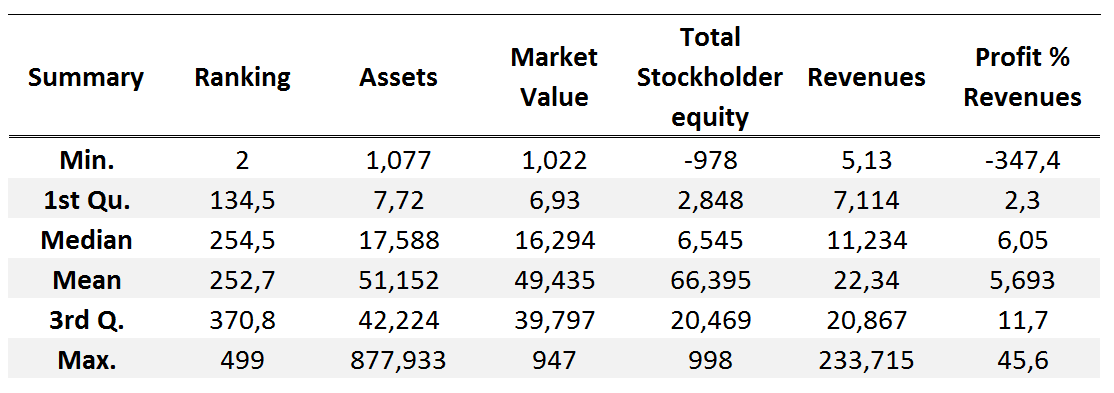
\includegraphics[scale=0.4]{../R/photos/01_summary.PNG} 
\end{table}

From this table we can see that even though some of the observations were removed from the cleansing the mean and the median are still very close to 250 and even though the first and the 500 websites are not included the way that the ranking is distributed is perfect for the rest of the analysis.\\
\begin{figure}[H]
\centering
\caption{Ranking}
\begin{center}
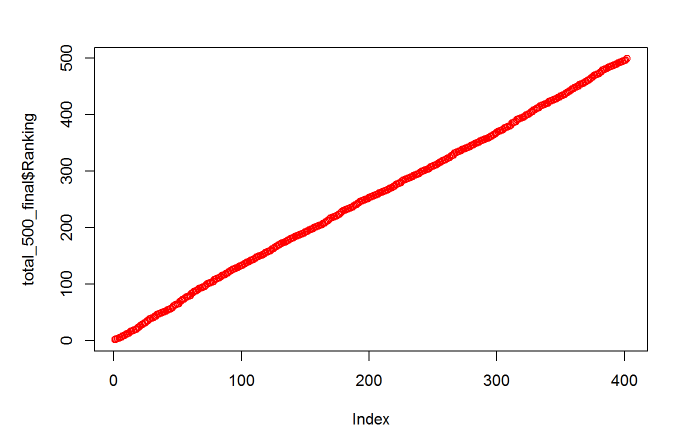
\includegraphics[scale=0.35]{../R/photos/4_2_ranking.png}  \\
\end{center}
\end{figure}
Regarding the Assets that are calculated in millions of dollars we can see that the min price that we can meet is 1 million dollars while the max price is 877 million dollars. Moreover the mean and the median are not very close to each other. This can mean that more than half of the companies at hand have less than 17 million in assets while due to the large gap between the min and the max price the mean is a lot bigger that this price.\\
\begin{figure}[H]
\centering
\caption{Assets}
\begin{center}
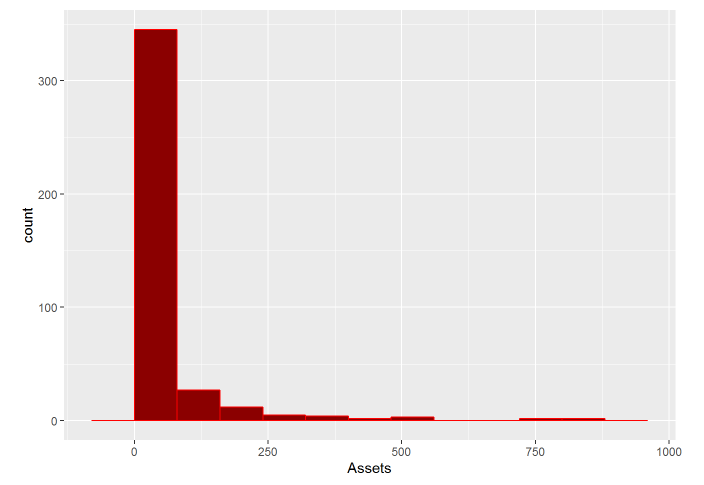
\includegraphics[scale=0.35]{../R/photos/4_2_assets.png}  \\
\end{center}
\end{figure}
Furthermore, the market value of the companies seems to have even larger deviation between the max and the min price and it actually follows the same logic as the assets.\\
\begin{figure}[H]
\centering
\caption{Market Value}
\begin{center}
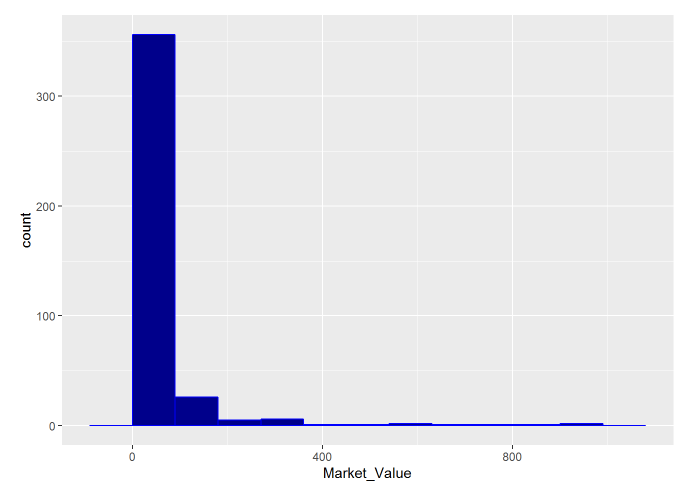
\includegraphics[scale=0.35]{../R/photos/4_2_market_value.png}  \\
\end{center}
\end{figure}
Moreover, the total stockholder equity variable has a min value of -978 millions and a max value of 998 millions. Again here the medium and the mean have a very large distance of almost 54 million dollars.\\
\begin{figure}[H]
\centering
\caption{Total stockholder equity}
\begin{center}
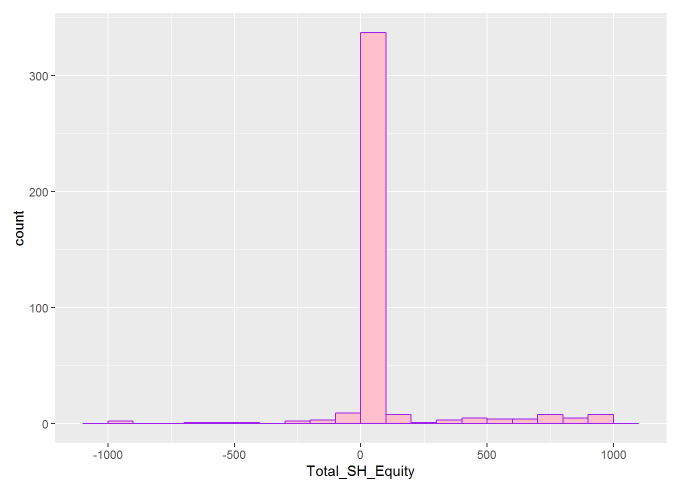
\includegraphics[scale=0.35]{../R/photos/4_2_equity.png}  \\
\end{center}
\end{figure}
Now regarding the revenues of each company we can see that they begin from 5 million dollars and reach 233 million dollars. Also here the mean and the median have a distance of 10 million dollars again due to the large deviation of prices.\\
\begin{figure}[H]
\centering
\caption{Revenues}
\begin{center}
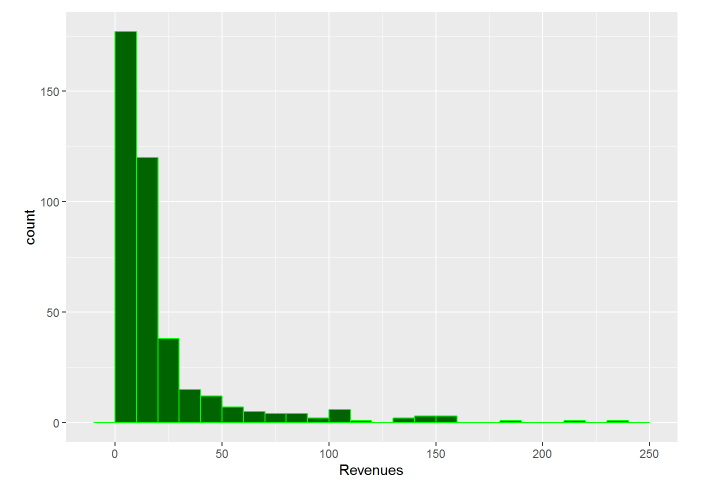
\includegraphics[scale=0.35]{../R/photos/4_2_revenues.png}  \\
\end{center}
\end{figure}
Finally, the profit per revenue variable shows the percentage of profit in regards to revenues. Here we can see that the min price is negative, which means that while this company has some revenues it doesn't actually have any profit. Here the biggest price is 45 while the mean and the median are very close to each other despite the big deviance between the min and the max.\\
\begin{figure}[H]
\centering
\caption{Profit \% Revenues}
\begin{center}
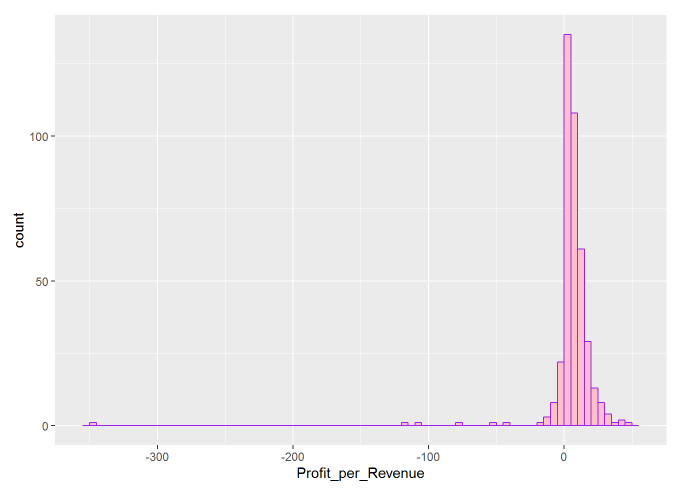
\includegraphics[scale=0.35]{../R/photos/4_2_ppp.png}  \\
\end{center}
\end{figure}
Now that we had a glimpse of the variables distribution we should see which one is more correlated to the ranking variable in order to see which variable we will use as the comparison metric. Since the Fortune 500 magazine is ranking the sites based on the revenues we expect to see that this variable will be the most correlated with the Ranking. Although we should also check the correlations of the other variables as well in order to be sure. In the following table we can see the correlation of the Ranking with each one of the Fortune 500 variables. The table was created by performing regression analysis with each variable against the ranking variable:
\begin{table}[H]
\centering
\caption{Ranking Regression models}
\begin{center}
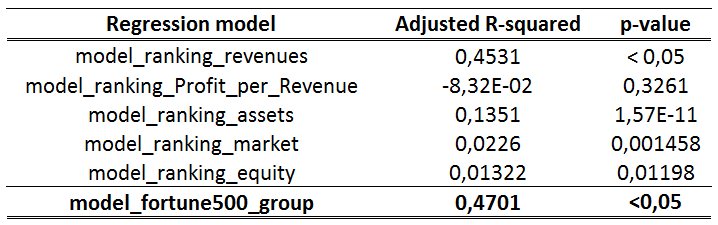
\includegraphics[scale=0.5]{../R/photos/4_2_reg_mod.png}  \\
\end{center}
\end{table}
Based on the above regression models that we ran we can conclude that the variable that we will use in order to see the influence of the websites variables in the company is the Revenues. As it is clear from the table that it has the best adjusted R square in relation to the ranking and a p-value lower than 0.05.\\
In the last line of the table we have performed a regression model for all the variables of the fortune 500 that we have downloaded using as the dependent variable again the ranking. Here we can see that the model has a little worse adjusted r square from the model we created for just the ranking and the revenues.\\
We can double check those finding with the help of the libraries corrplot and caret. We run a correlation plot with all the variables we have seen above. Moreover, the code that was used to create these tables is available in the Appendix.\ref{r2}:
\begin{table}[H]
\centering
\caption{Fortune variables correlation plot}
\begin{center}
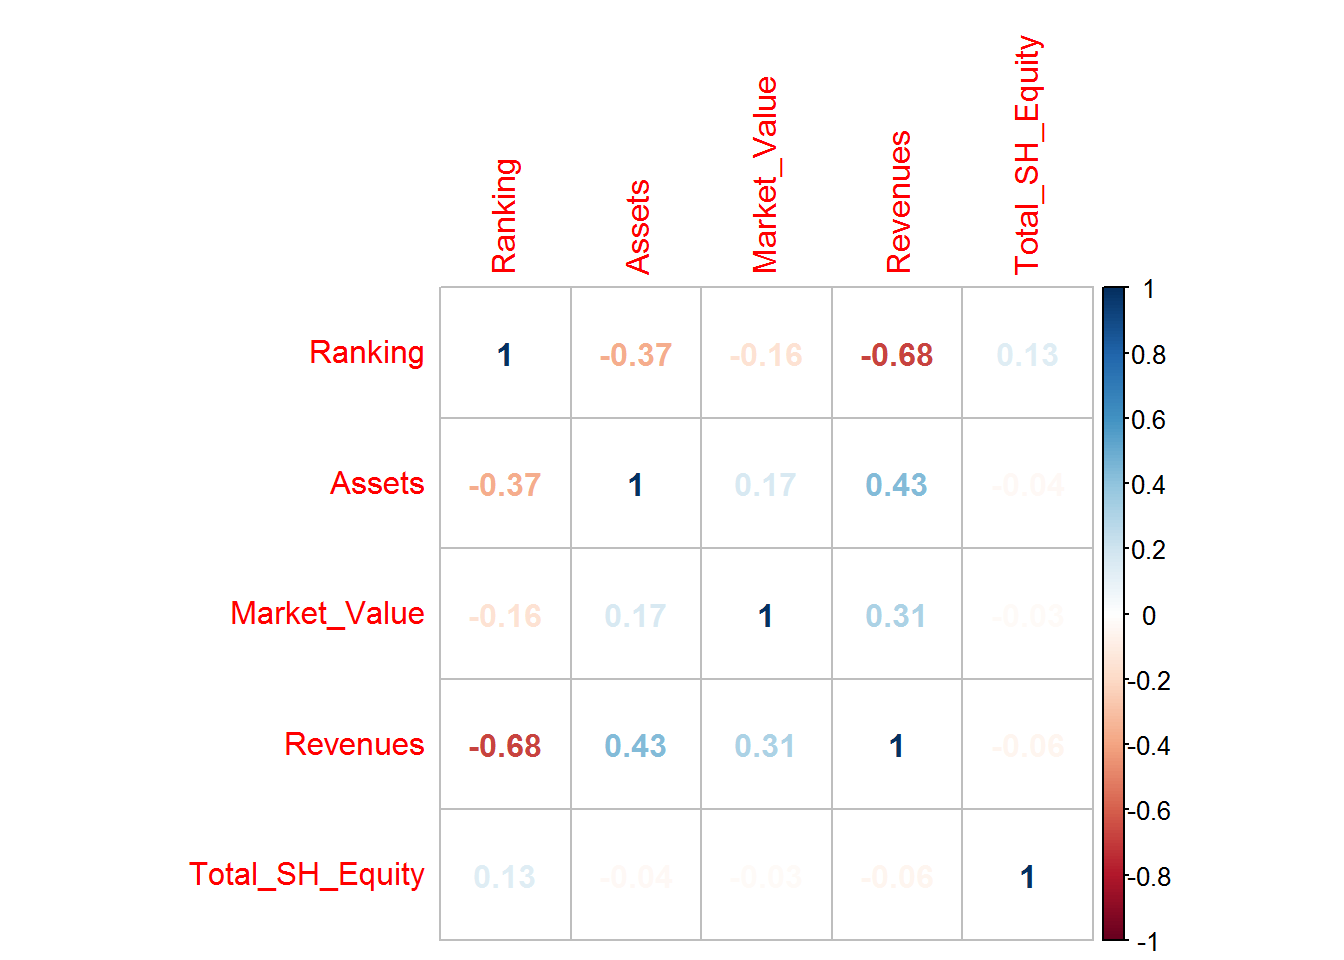
\includegraphics[scale=0.5]{../R/photos/09_rank_corplot_f500.png}   \\
\textit{From the table we see that the strongest negative correlation is between Ranking and Revenues as we already have seen.}
\end{center}
\end{table}
\newpage
\section{Social media variables analysis}
Now that we have seen the correlations between the fortune variables and we reached to the conclusion that the metric that is more correlated to the ranking is the revenues we will proceed with analysing the social media variables to see how they are distributed and then to see how they are correlated with the Revenues variable.
\begin{figure}[H]
\centering
\caption{Social media (link existence on the site)}
\begin{center}
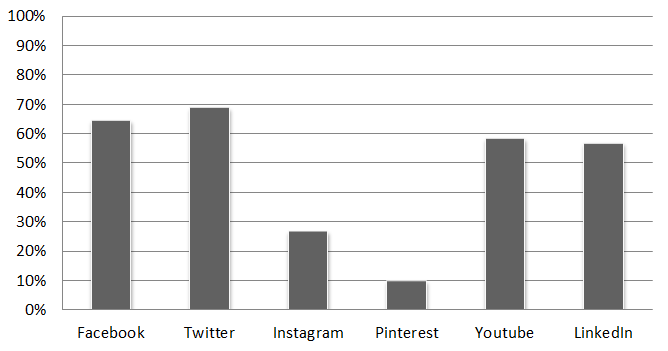
\includegraphics[scale=0.6]{../R/photos/10_socialmedia.png}
\end{center}
\end{figure}
From the above figure we can see that the most widely used social media link in the companies web page is the twitter, followed in close proximity by the facebook link. More precicly while almost the 65\% of the companies that we are examining have facebook links on their home page, almost the 67\% of the companies have Twitter links on their home page.\\
Furthermore regarding the social media that are less used by the companies we see that only the 25\% of the companies that we are examining have instagram links on their home page, while when it comes to pinterest only a small 10\% of the companies have links to this social media on their home page.\\
Finally the 58\% of the companies that we are examining have YouTube links on their home page and the 57\% of the companies that we are examining have YouTube links on their home page.\\
Now that we have seen how widely or not the social media links appear in the web pages under examination we have to check the correlation with the revenue variable. In the below table we can see the regression model for each one of the social media against the revenues variable and also the regression model with all the social media as a group against the revenues variable.
\begin{table}[H]
\centering
\caption{Social media regression models}
\begin{center}
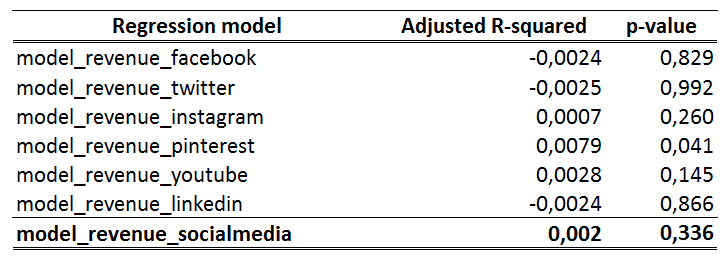
\includegraphics[scale=0.5]{../R/photos/4_2_reg_sm.png}  \\
\end{center}
\end{table}
From the regression models we can see that the only one with a p-value smaller than 0,05 is the model with the pinterest variable. Nevertheless even though the p-value is adequate the adjusted R-squared is extremely small. From these regression models we can see that the existence or not of a social media link is not correlated with the company's success. We didn't see any improvement not even in the multi regression model where we included all the social media variables.\\
In order to conclude the analysis of the social media with the help again of the corrplot library we will create also a correlation table with all the variables in order to duplicate our results.
\begin{table}[H]
\centering
\caption{Social media correlation table}
\begin{center}
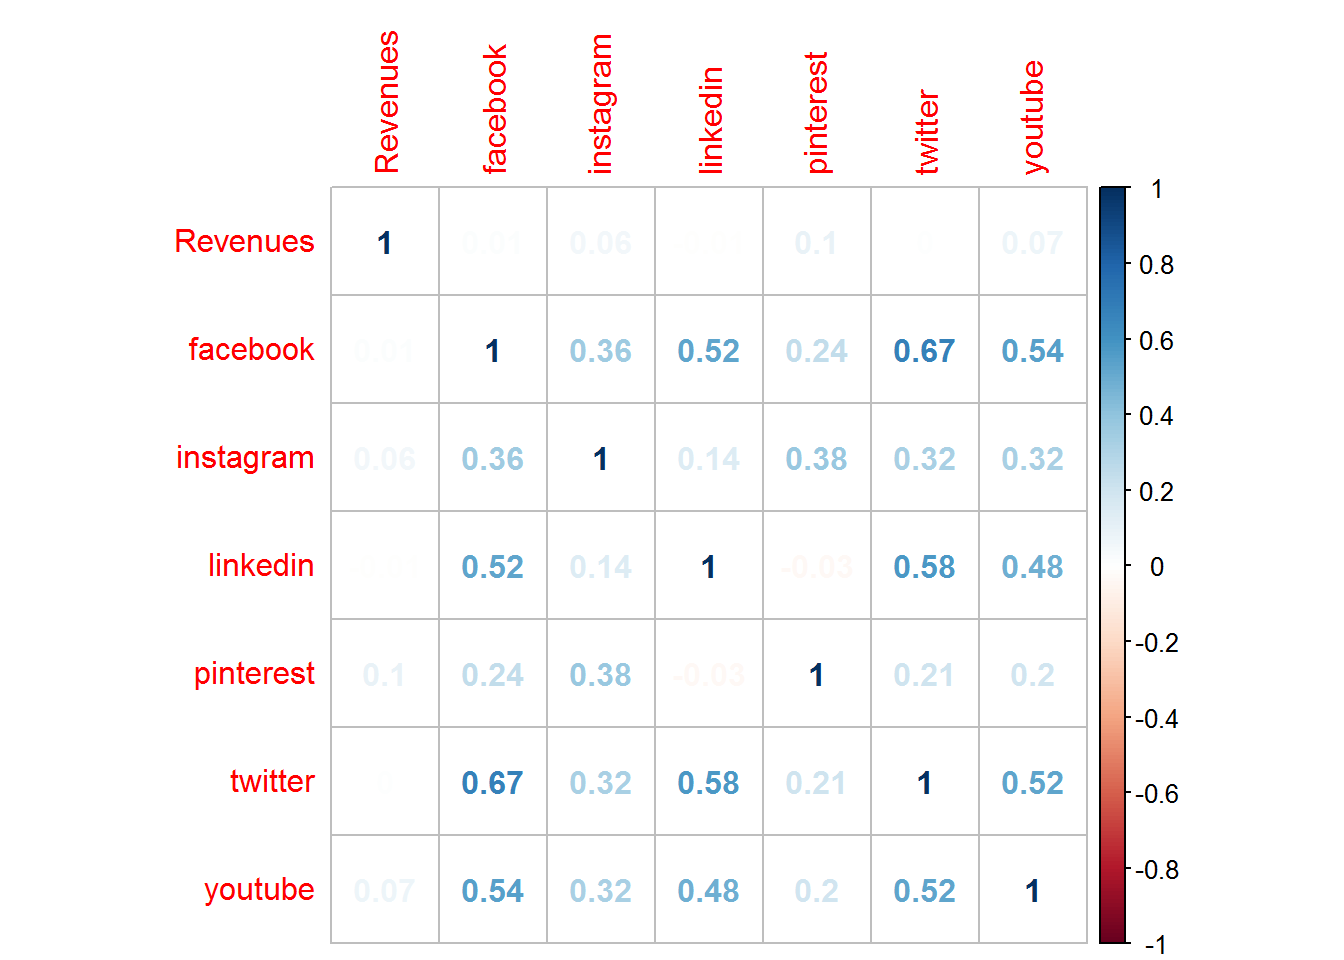
\includegraphics[scale=0.5]{../R/photos/22_REV_SM.png}  \\
\end{center}
\end{table}
From the correlation table we can see that the Revenues do not have any high correlation with the social media variables as we already have seen from the regression models. Again we can see that even if it is small and not important the highest correlation is again with the pinterest variable.\\
Moreover what we can observe here is that the existence of specific social media is highly correlated with the existence of other social media. For instance there is a 69\% correlation between the existence of a twitter link and a facebook link, which can be explained due to the fact that the majority of the sites use both of these social media links.\\
The code we used to create this chart is available in the Appendix.\ref{r3}

\section{Links variables analysis}
The category that we are going to analyse now is the mink variables. More specifically we are going to analyse the distribution of the internal, external and total links and of course their correlation with each other and with the Revenues. First step is to see the distribution of the variables at hand:
\begin{table}[H]
\centering
\caption{Links variables summary}
\begin{center}
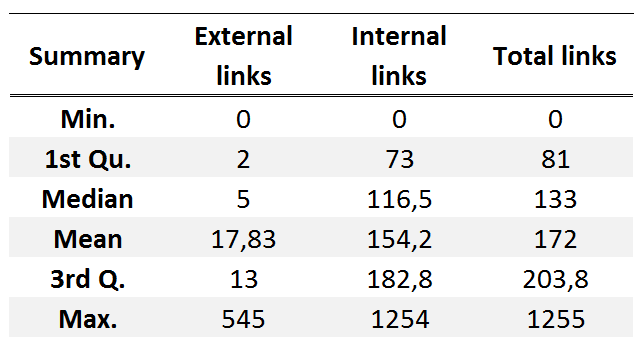
\includegraphics[scale=0.4]{../R/photos/4_2_reg_links.png}  
\end{center}
\end{table}
From the summary table we can see that the external links are distributed between 0 to 545. The mean and the median are not very close. Also we can see that the 75\% of the sites have 13 or less external links.\\
\begin{figure}[H]
\centering
\caption{External links distribution}
\begin{center}
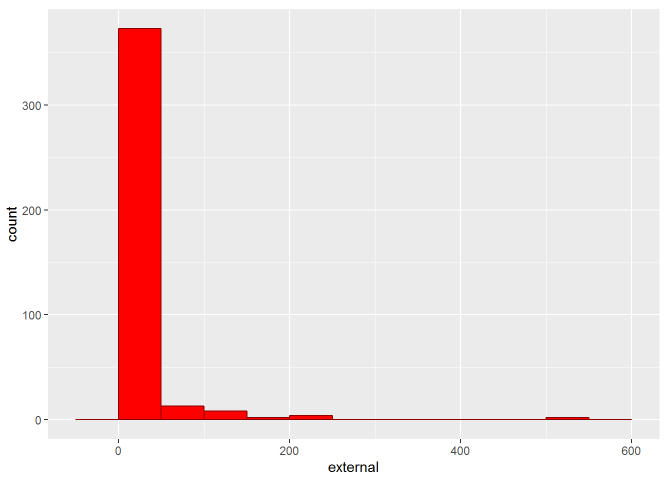
\includegraphics[scale=0.4]{../R/photos/4_2_ex.png}  
\end{center}
\end{figure}
Regarding the internal links we can see that the prices are distributed in a more wide range between 0 and 1254 with the mean being 154 and the median 116.\\
\begin{figure}[H]
\centering
\caption{Internal links distribution}
\begin{center}
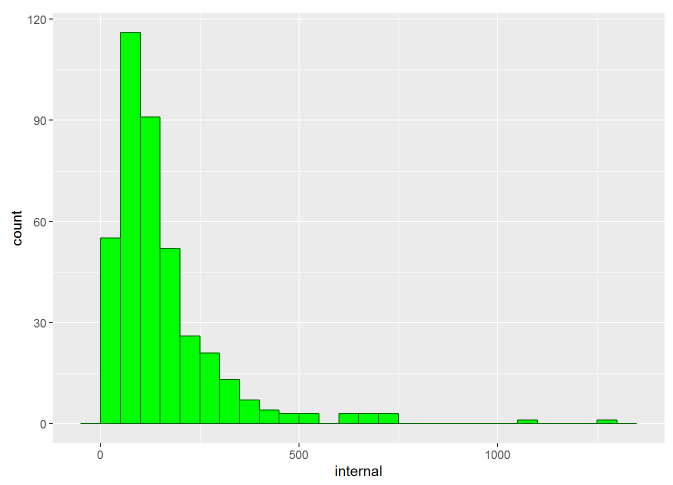
\includegraphics[scale=0.4]{../R/photos/4_2_in.png}  
\end{center}
\end{figure}
Finally the total links distribution is more close to the internal links one with the range being from 0 to 1255 and the mean 172 while the median is 133.\\
\begin{figure}[H]
\centering
\caption{Total links distribution}
\begin{center}
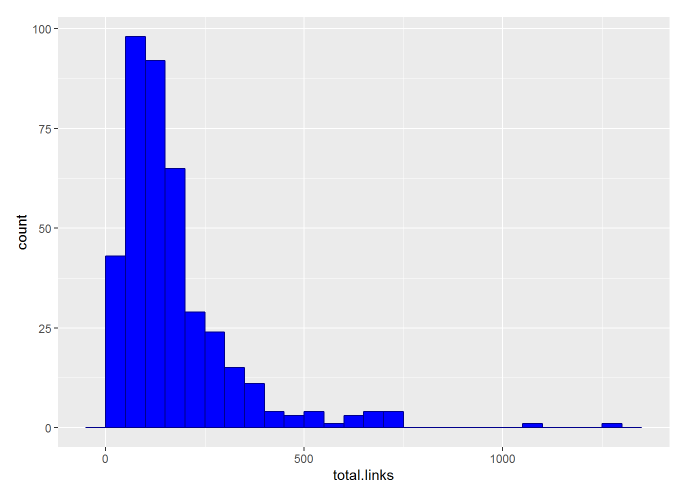
\includegraphics[scale=0.5]{../R/photos/4_2_tl_dist.png}  
\end{center}
\end{figure}
Now that we saw the distribution of the variables we should see their correlation with the revenues variable by performing regression analysis with each variable and then with all the 3 variables together against the revenues one.\
\begin{table}[H]
\centering
\caption{Links regression models}
\begin{center}
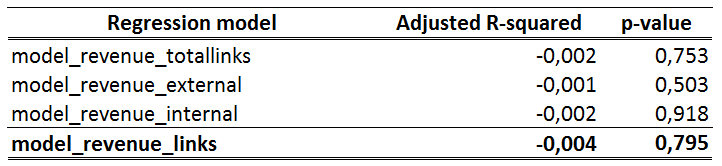
\includegraphics[scale=0.6]{../R/photos/4_2_reg_mod_links.png}
\end{center}
\end{table}
From the regression models we can see that non of the models show any correlation between the revenues variable and the variables at hand. In order to double check we will again create a correlation table:
\begin{table}[H]
\centering
\caption{Links correlation table}
\begin{center}
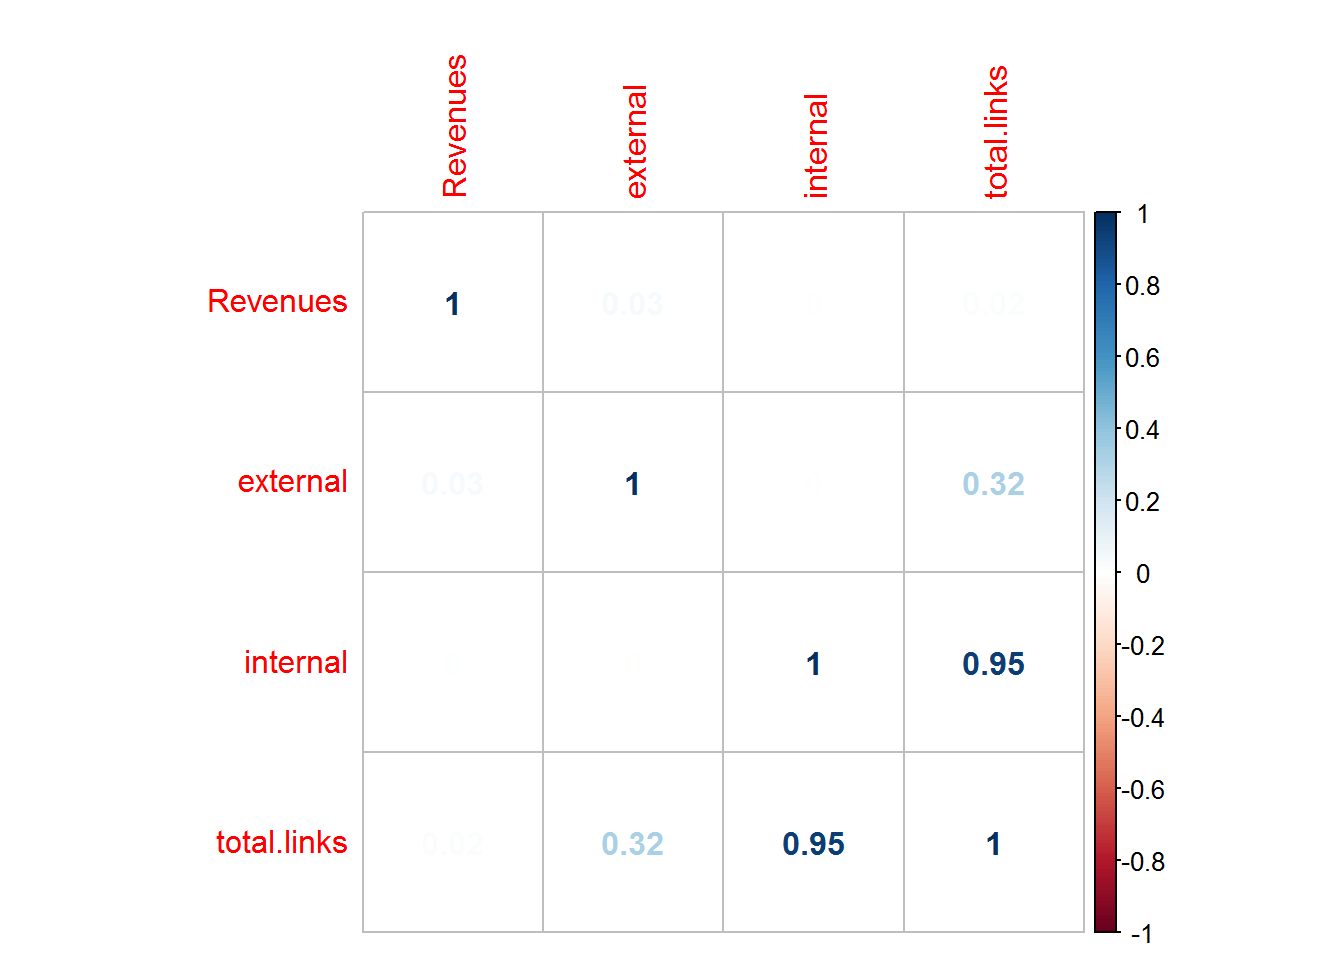
\includegraphics[scale=0.6]{../R/photos/29_rev_cor_links.png}  \\
\end{center}
\end{table}
From the correlation table we can see that the observation we made based on the regression models that we created is true. We do not se any high correlation with the revenues variable. What we can see is an extremely high correlation with the internal links and the total links which was expected since the total links is the combination of the external and the internal ones and the total links have a very similar distribution with the internal links as we show before.The code for this section is available in the Appendix.\ref{r4}
\section{Loading time variable analysis}
The loading time of the sites is a very important key performance indicator usually in website performance so it is very interesting to see if it has any strong correlation with the revenues variable. The first step is to check the variables distribution:
\begin{figure}[H]
\centering
\caption{Loading time distribution}
\begin{center}
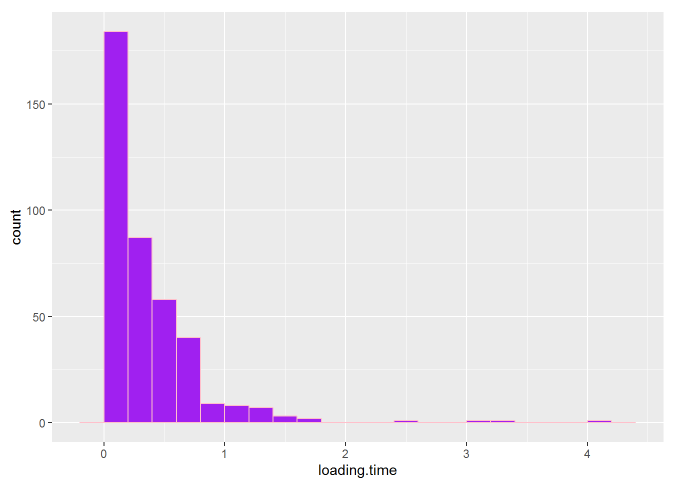
\includegraphics[scale=0.4]{../R/photos/30_ld_dist.png}
\end{center}
\end{figure}
From the above figure we can see that the range of the loading time for the companies at hand is between 0 and 4.06 with the mean price being 0.36 and the median being 0.26.\\
The next step is to create a regression model against the revenues variable to see if there is any correlation.
\begin{table}[H]
\centering
\caption{Loading time regression model}
\begin{center}
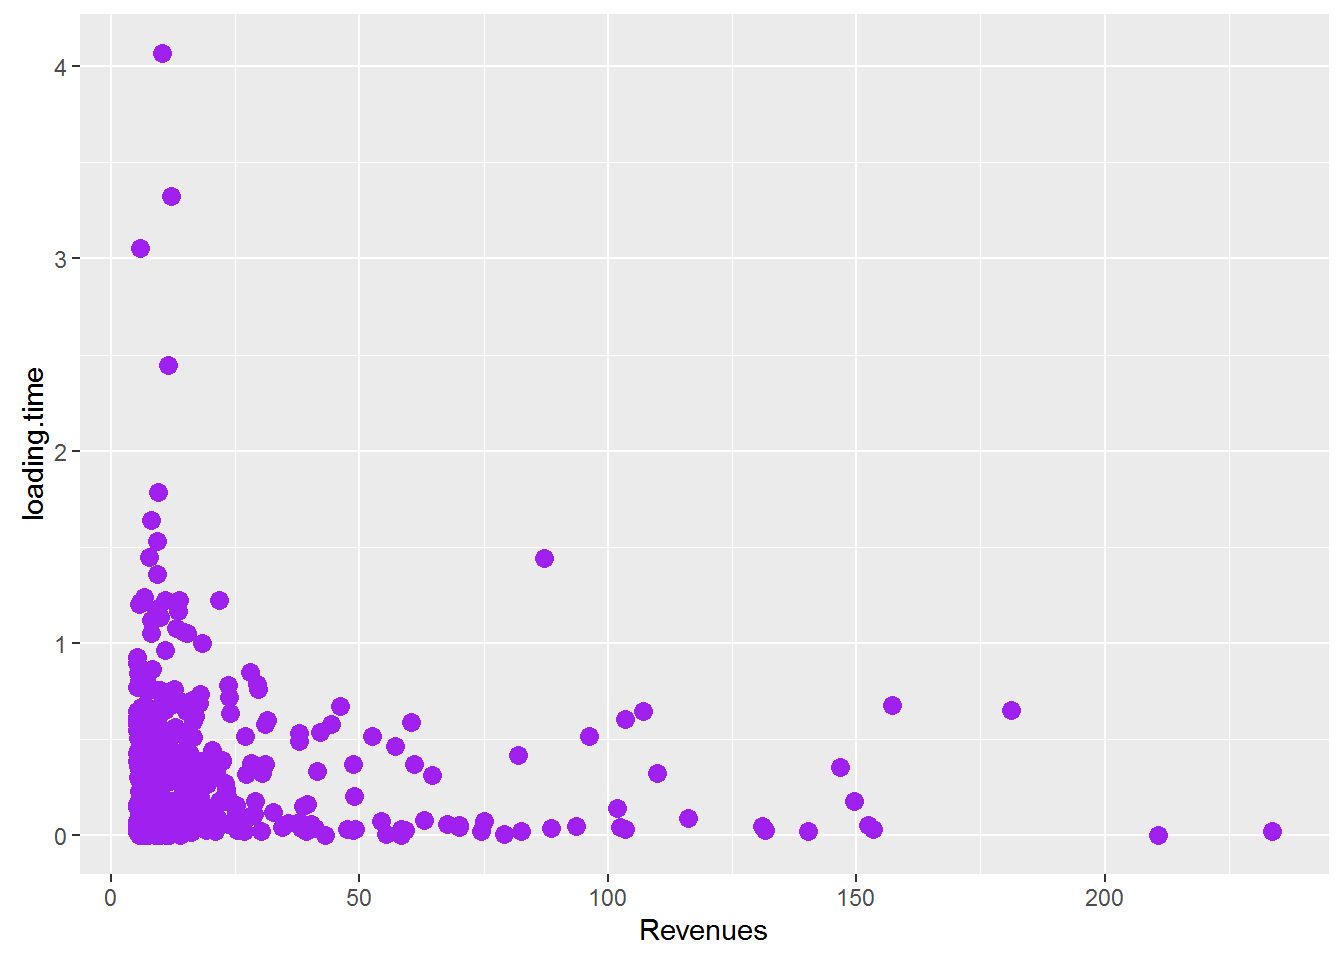
\includegraphics[scale=0.9]{../R/photos/31_ld_rev.png}
\end{center}
\end{table}
From the regression model we can see that the p-value is smaller than 0.05 and the Adjusted R-square is 0.012 which is very low again. The code for this table is available in the Appendix.\ref{r5}
\section{Content variable analysis}
The next step is to analyse the distribution of the variables that are related to the content and the text of the websites in relation to the Revenues of the companies at hand. As we explained in the Python chapter\ref{M:Content} we gathered 3 variables that are related to the grammatical overview of the text that is being used in the sites - which are the numbers of words, the number of unique words and the number of sentences - and 2 variables that are trying to explain if the content of this text is comprehensible from the majority of the users or not. Following below we have the table with the distributions of those variables prices across the sites under examination:
\begin{table}[H]
\centering
\caption{Content variables distribution}
\begin{center}
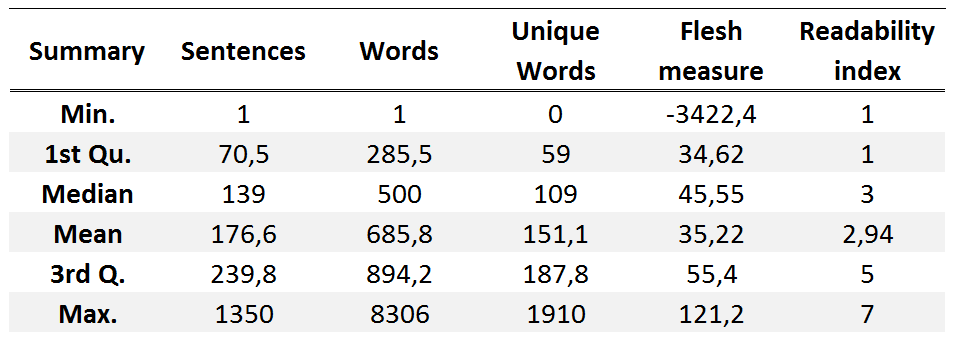
\includegraphics[scale=0.4]{../R/photos/4_2_dist_content.png}
\end{center}
\end{table}
From the distribution table we can see that the sentences in each site are between 1 and 1350 with the mean being 176 and the median 139.
\begin{figure}[H]
\centering
\caption{Sentences distribution}
\begin{center}
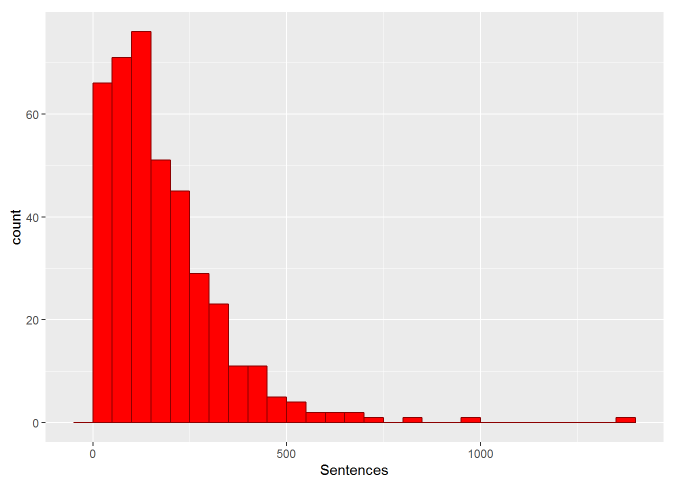
\includegraphics[scale=0.4]{../R/photos/4_2_s.png}   
\end{center}
\end{figure}
The distribution of words as it was expected is wider than the sentences. It begins from only 1 word and reaching 8306 words in a site. Although the max price is an outsider if we take into account that the mean is 685 and the median 500.
\begin{figure}[H]
\centering
\caption{Words distribution}
\begin{center}
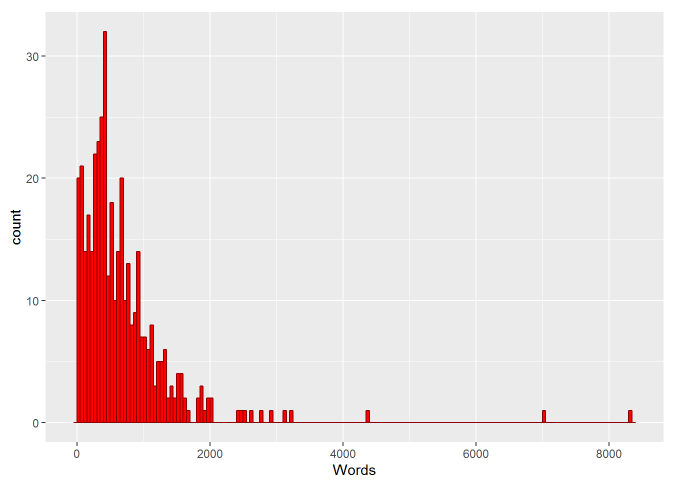
\includegraphics[scale=0.4]{../R/photos/4_2_w.png}   
\end{center}
\end{figure}
The unique words we expect to be a lot lower than the total words and that's exactly the case. The unique words are between 0 to 1910 with a mean of 151 and a median of 109.
\begin{figure}[H]
\centering
\caption{Unique words distribution}
\begin{center}
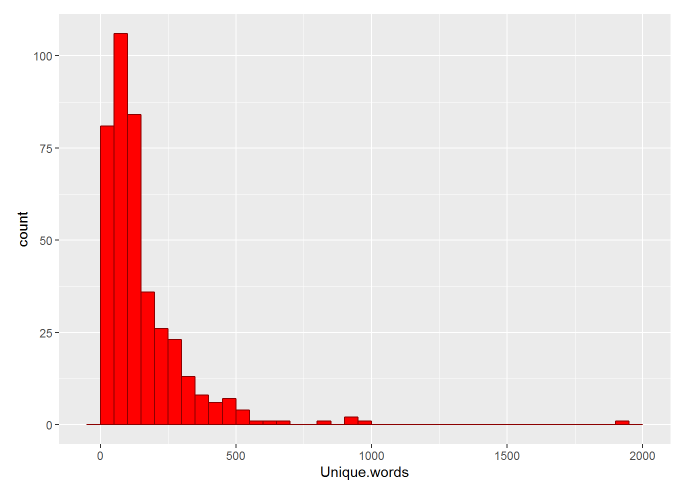
\includegraphics[scale=0.4]{../R/photos/4_2_uw.png}   
\end{center}
\end{figure}
Now regarding the flesh measure we can see that the price range is between -3422 to 121. Although in order to better understand and comprehend the explanation of the flesh measure we created the readability index as well which goes from 1 (which means very easy to read) to 7 which is very confusing text. The mean and the median are close to 3. We can see in the below figure that the most companies choose to have a very easily readable text:
\begin{figure}[H]
\centering
\caption{Readability distribution}
\begin{center}
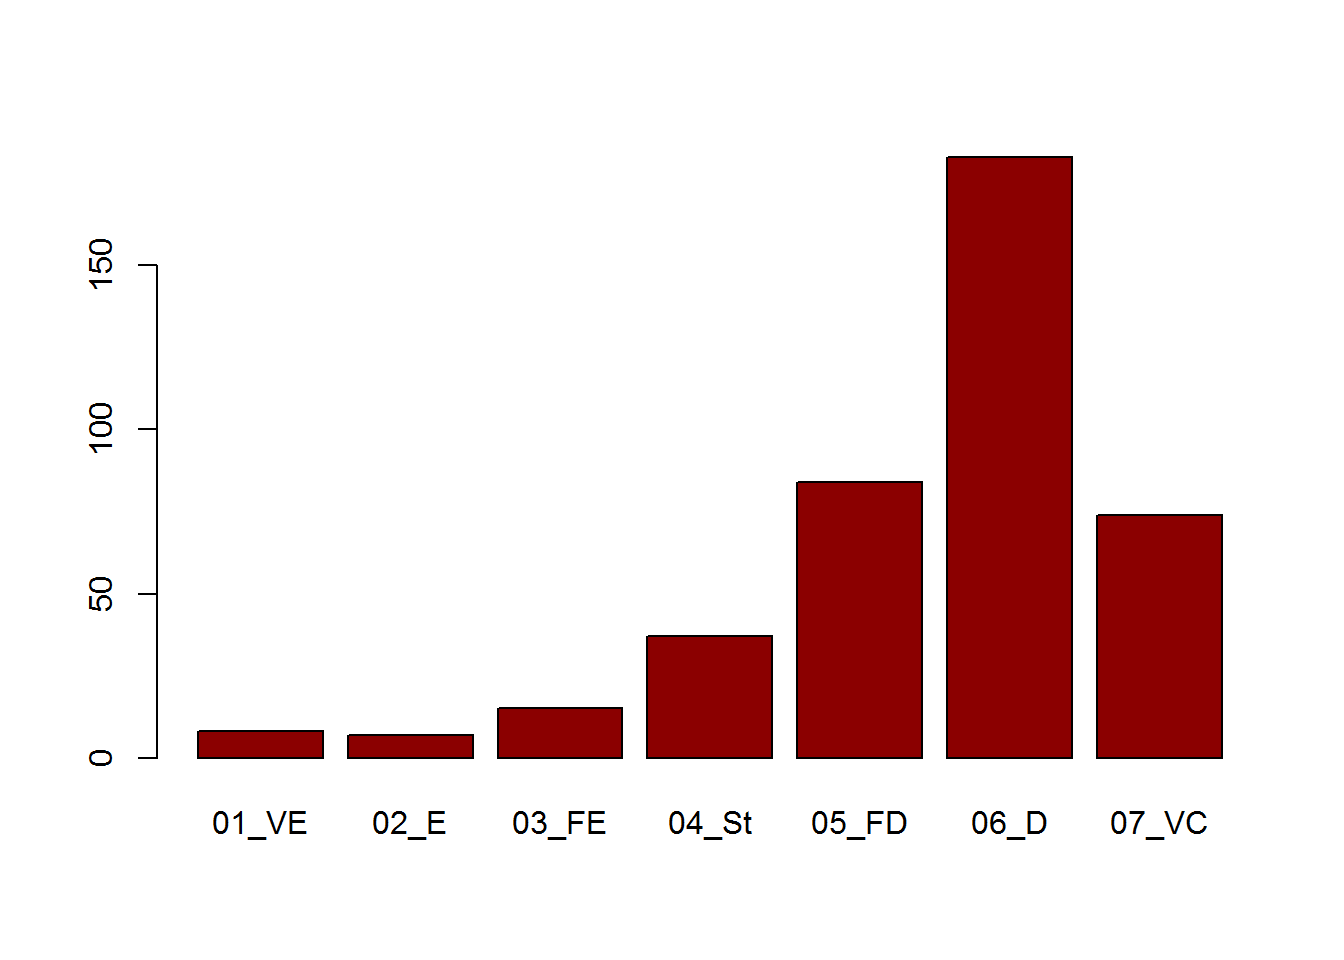
\includegraphics[scale=0.5]{../R/photos/41_read_dist.png}   
\end{center}
\end{figure}
Now that we have seen the distribution of the variables at hand we should also check their correlation with the revenues variable by performing simple regression models with the dependent variable being the revenues and also multi regression models with all the variables of the group plus the loading time variable from the previous sector to see if in combination the variables are correlated more with the revenues. In the following table we can see the results of these regression models:
\begin{table}[H]
\centering
\caption{Content variables regression models}
\begin{center}
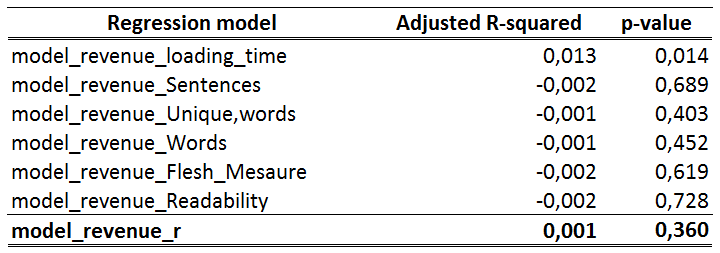
\includegraphics[scale=0.6]{../R/photos/4_2_reg_content.png}   \\
\end{center}
\end{table}
From the above table we can see that the only model with a p value lower than 0,05 is the loading time model which we have already seen in the previous chapter and we said that regardless the fact that the p value is low the adjusted r-square is too low so as to see a specific correlation. Moreover we will do here as well a correlation plot to see if we will see the same results there as well:
\begin{table}[H]
\centering
\caption{Correlation table}\label{lod}
\begin{center}
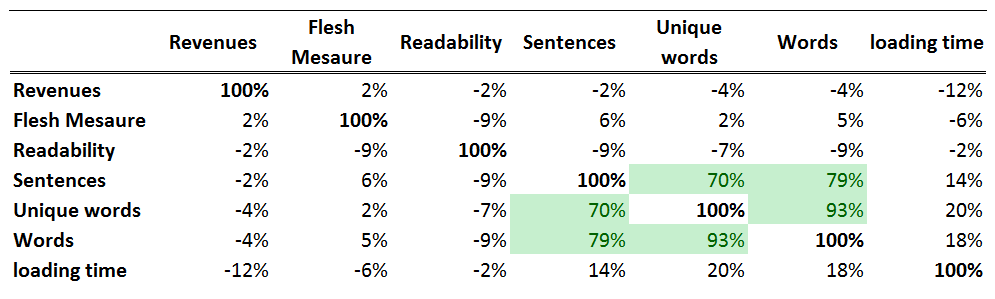
\includegraphics[scale=0.45]{../R/photos/43b_read_cor.png}    
\end{center}
\end{table}
From the correlation table we can also observe that the three variables we examined regarding the text of the websites are highly correlated with each other which as we already explained is an expected outcome.\\
Moreover the biggest correlation is -12\% with the loading time and the revenues as we have already seen from the simple regression models we created. The code for this section is available in the Appendix.\ref{r6}

\section{HTML validation variables analysis}
During the extraction of the HTML validation variables we created 4 different metrics: the "number of errors", the "number of warnings", the "non document error" and "the page opened" one. In this section we are going to analyse the distributions of the three of those variable since the variable "the page opened" has the same price across all websites under examination and it would not offer us any further assistance in this analysis. In the below table we can see the distribution of the three html variables:
\begin{table}[H]
\centering
\caption{HTML validation variables distribution}
\begin{center}
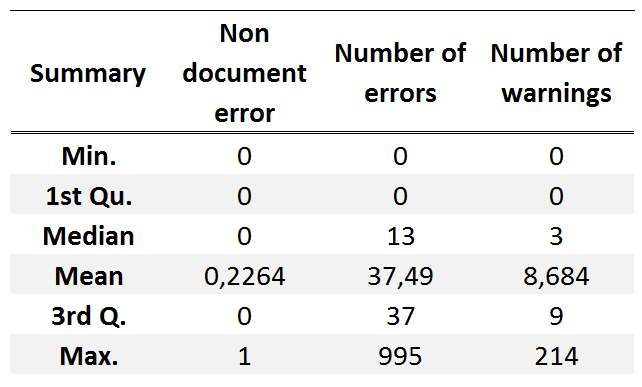
\includegraphics[scale=0.5]{../R/photos/4_2_sum_html.png}    
\end{center}
\end{table}
From the above table we can see that the non document error can take either 1 or 0 prices and each mean is 0.22.\\
\begin{figure}[H]
\centering
\caption{Non document error distribution}
\begin{center}
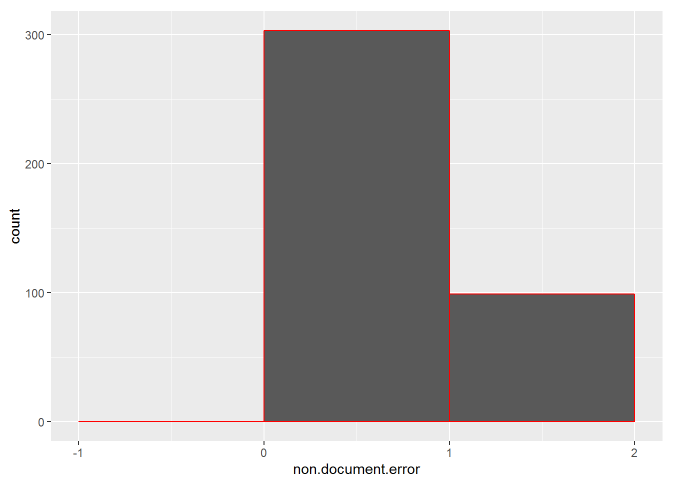
\includegraphics[scale=0.4]{../R/photos/4_2_n.png}   
\end{center}
\end{figure}
The number of errors variable has a range of 0 to 995 while the 75\% of the observations are equal or less to 37 errors which is almost equal to the mean while the median is 13.\\
\begin{figure}[H]
\centering
\caption{Number of errors distribution}
\begin{center}
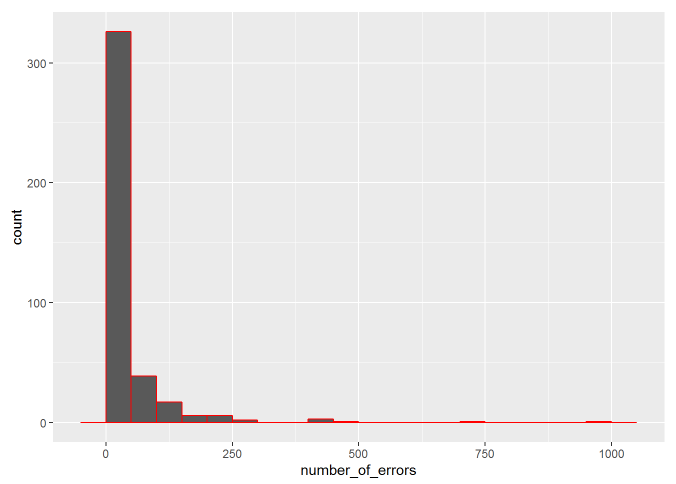
\includegraphics[scale=0.4]{../R/photos/4_2_ne.png}   
\end{center}
\end{figure}
The number of warning are less than the number of errors and their range is from 0 to 214 with a mean 8.6 and a median 3. Again here the mean is very close to the 3rd quarter value which is 9 and means that the 75\% of the variables have equal or less warnings than 9.\\
\begin{figure}[H]
\centering
\caption{Number of warnings distribution}
\begin{center}
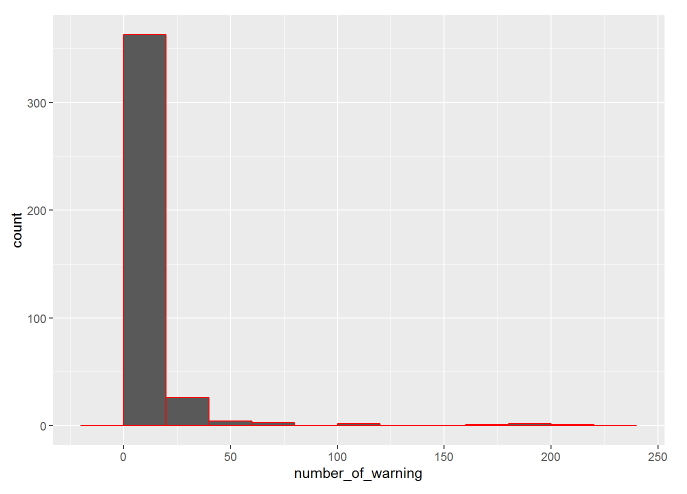
\includegraphics[scale=0.4]{../R/photos/4_2_nw.png}   
\end{center}
\end{figure}
Now that we have understand the distribution of the html validation variables we should perform the simple and the multiple regression models to see the correlation of those variables with the companies revenues in an atomic level but also as a group of variables. In the below table we can see the results of the regression models that were performed:
\begin{table}[H]
\centering
\caption{Html validation variables regression models}
\begin{center}
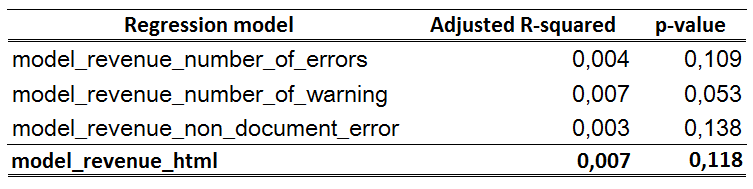
\includegraphics[scale=0.6]{../R/photos/4_2_reg_html.png}    \\
\end{center}
\end{table}
From the regression models we can see that the only one that has 0.05 p value is the one with the number of warning but still it has a very low Adjusted R-square. In order to double check the results we will create a correlation table as well with the help of the library corrplot:
\begin{table}[H]
\centering
\caption{Html validation correlation table}
\begin{center}
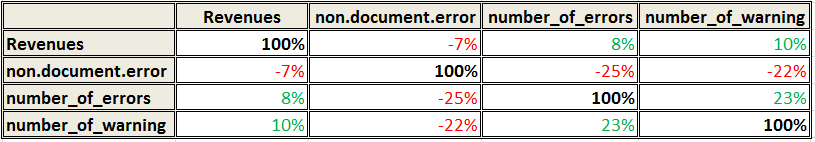
\includegraphics[scale=0.6]{../R/photos/51b_html_cor.PNG} 
\end{center}
\end{table}
From the correlation table we can firstly see that the regression models where correct as the biggest correlation is between the number of warnings variable but still the correlation is pretty small. Moreover we can also see that there is not any important correlation between the variables as well. The code for this section is available in the Appendix\ref{r7} 
\section{Image variables analysis}
Last but not least we should analyse the distribution of the different types of images that are being used on the websites we are examining and also compare the total images with the Revenues to see their correlation.
\begin{table}[H]
\centering
\caption{Image variables distribution}
\begin{center}
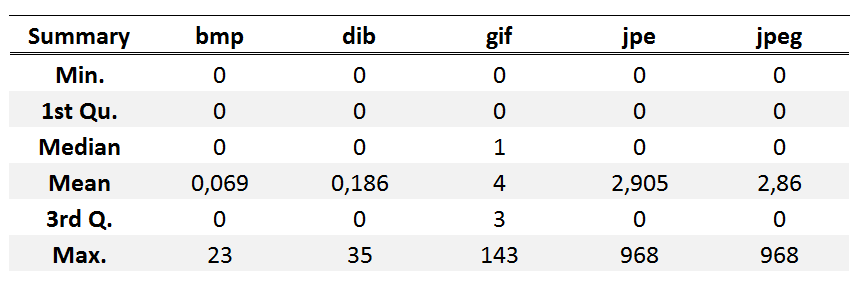
\includegraphics[scale=0.5]{../R/photos/4_2_sum_img_1.png}    
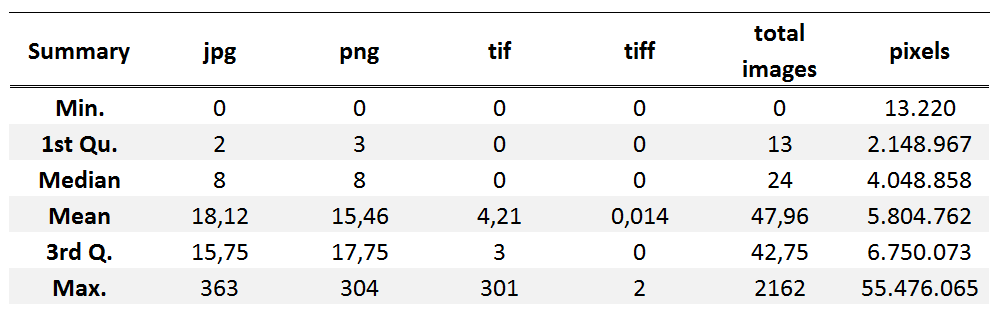
\includegraphics[scale=0.5]{../R/photos/4_2_sum_img_2.png}    
\end{center}
\end{table}
From the above tables we can see that the bmp image type price range is between 0 to 23 with a median 0 and a mean 0.069.
\begin{figure}[H]
\centering
\caption{Bmp format distribution}
\begin{center}
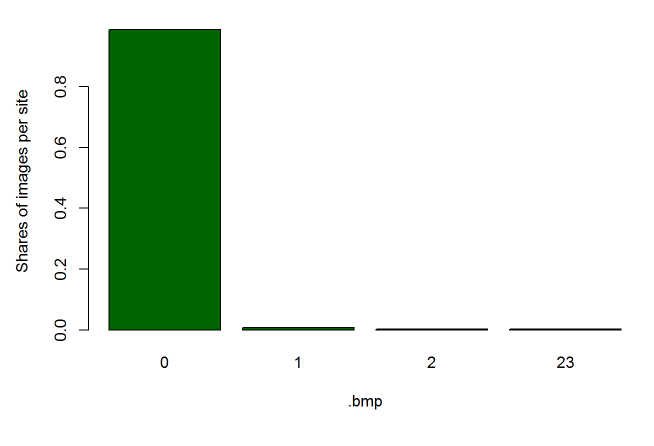
\includegraphics[scale=0.4]{../R/photos/4_2_bmp.png}   
\end{center}
\end{figure}
The dib image type has a bigger range between 0 to 35 with a same median 0 and a mean 0.186.
\begin{figure}[H]
\centering
\caption{Dib format distribution}
\begin{center}
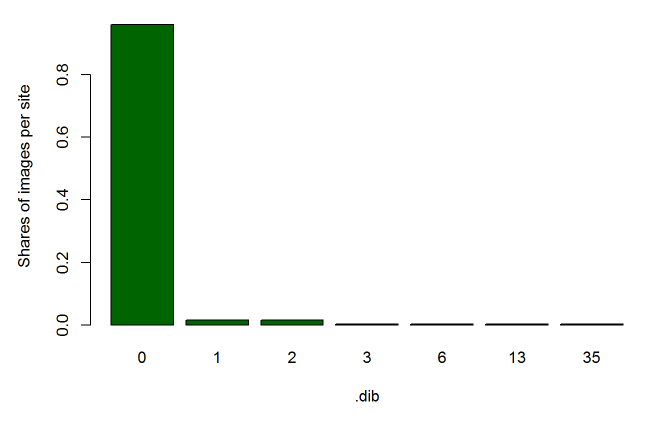
\includegraphics[scale=0.4]{../R/photos/4_2_dib.png}   
\end{center}
\end{figure}
The gif image type has a wider range of 0 to 143 with a median 1 and a mean 4.
\begin{figure}[H]
\centering
\caption{Gif format distribution}
\begin{center}
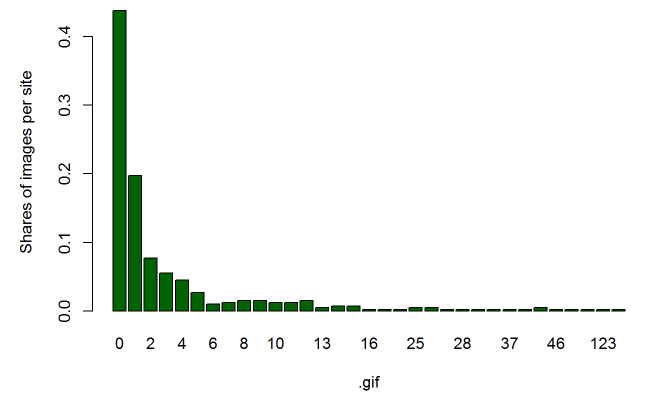
\includegraphics[scale=0.4]{../R/photos/4_2_gif.png}   
\end{center}
\end{figure}
The jpe image type has an even bigger range between 0 to 968 with a median 0 and mean 2.9.
\begin{figure}[H]
\centering
\caption{Jpe format distribution}
\begin{center}
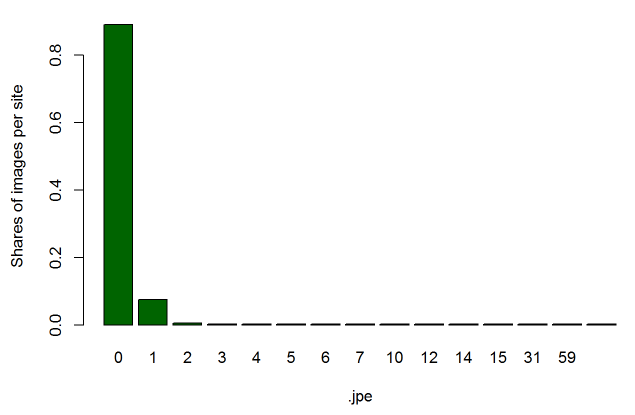
\includegraphics[scale=0.4]{../R/photos/4_2_jpe.png}   
\end{center}
\end{figure}
Similar distribution follows also the jpeg format with the only difference being that here the mean is 2.8.
\begin{figure}[H]
\centering
\caption{Jpeg format distribution}
\begin{center}
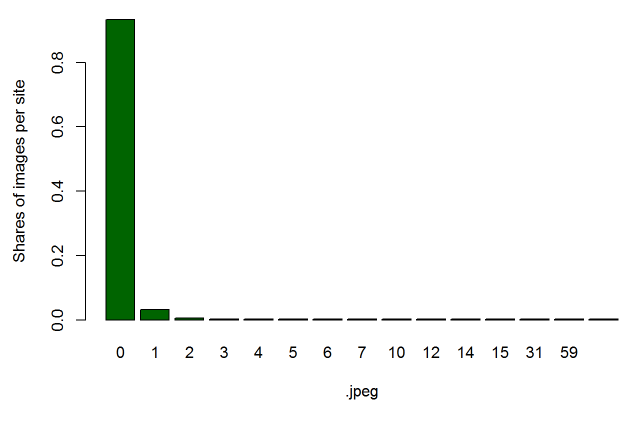
\includegraphics[scale=0.4]{../R/photos/4_2_jpeg.png}   
\end{center}
\end{figure}
The jpg format has a smaller range of 0 to 363 with a bigger median 8 and a mean of 18.
\begin{figure}[H]
\centering
\caption{Jpg format distribution}
\begin{center}
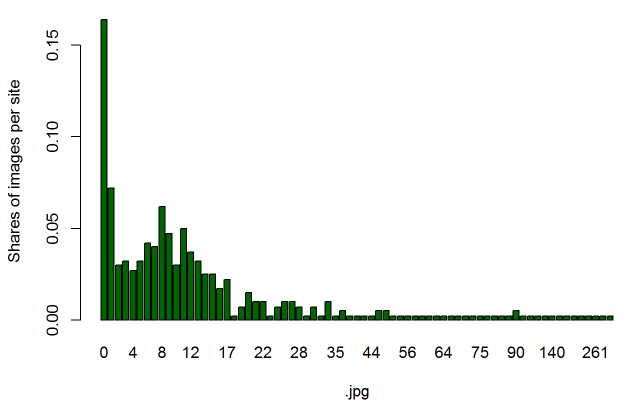
\includegraphics[scale=0.4]{../R/photos/4_2_jpg.png}   
\end{center}
\end{figure}
The png format is very similar to the jpg with a range from 0 to 304 and a median 8 and a mean 15.46.
\begin{figure}[H]
\centering
\caption{Png format distribution}
\begin{center}
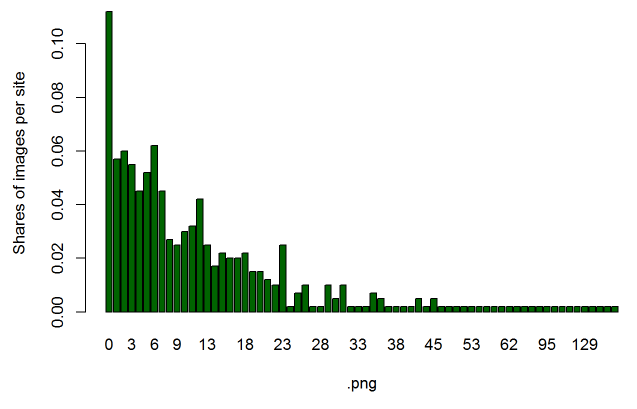
\includegraphics[scale=0.4]{../R/photos/4_2_png.png}   
\end{center}
\end{figure}
The tif format while has a similar range with the previous 2 formats from 0 to 301 the mean is quite smaller 4.21 and the median is 0.
\begin{figure}[H]
\centering
\caption{Tif format distribution}
\begin{center}
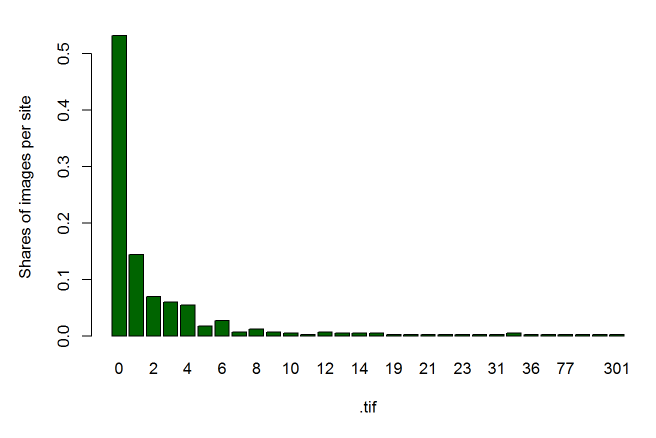
\includegraphics[scale=0.4]{../R/photos/4_2_tif.png}   
\end{center}
\end{figure}
The tiff format has a range of 0 to 2 which means that is not used in abundance from the websites at hand. The mean and the median are close to 0 that means that most of the sites are not using this format at all.
\begin{figure}[H]
\centering
\caption{Tiff format distribution}
\begin{center}
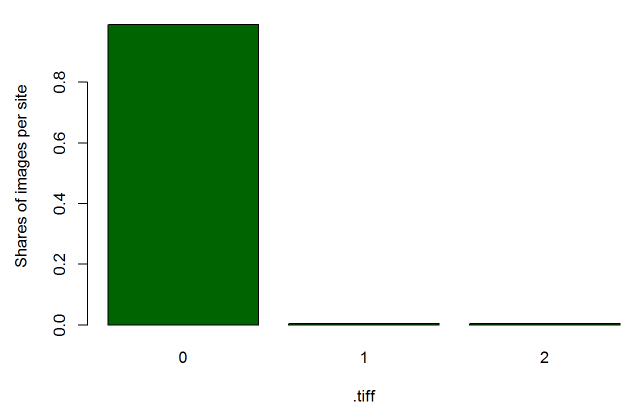
\includegraphics[scale=0.4]{../R/photos/4_2_tiff.png}   
\end{center}
\end{figure}
The total images us the results from all the images we have selected and we can see that the variable has a range from 0 to 2162 with a median 34 and a mean 47. The 75\% of the websites use 42 or less images in their home page.
\begin{figure}[H]
\centering
\caption{Total images distribution}
\begin{center}
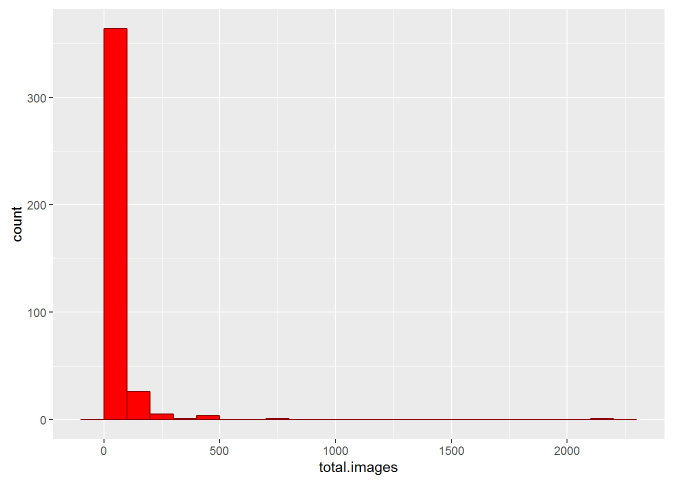
\includegraphics[scale=0.4]{../R/photos/4_2_tim.png}   
\end{center}
\end{figure}
Finally the pixels variable has a range from 13220 to 55 million pixels per site. With a median of 4 million and a mean of 5 million pixels. The 75\% of the sites have 6 million pixels or less.
\begin{figure}[H]
\centering
\caption{Pixels distribution}
\begin{center}
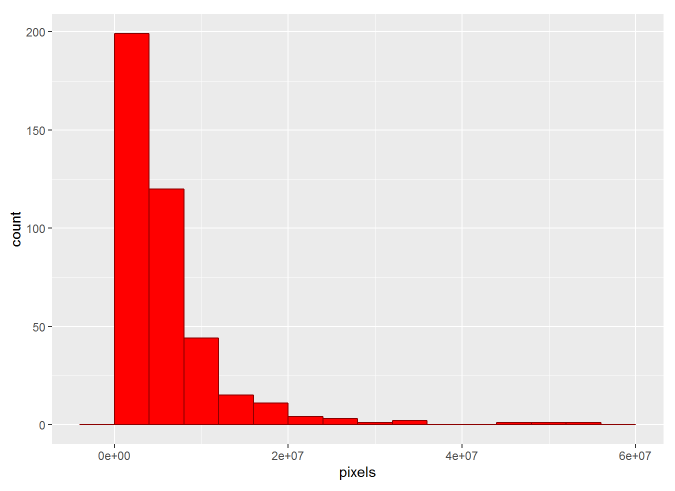
\includegraphics[scale=0.4]{../R/photos/4_2_pix.png}   
\end{center}
\end{figure}
Now that we show the distribution of the variables in this category we can now proceed with the creation of the simple regression models and then with a multiple regression models that will contain as independent variables all the variables of the group and as dependent variable the revenues. In the below table we can see the results of the regression models that were created:
\begin{table}[H]
\centering
\caption{Image variables regression models}
\begin{center}
\includegraphics[scale=0.6]{../R/photos/4_2_reg_img.png}    
\end{center}
\end{table}
From the regression models we can see that none of the models we created have a p-value lower than 0,05. Nevertheless the models for the dib format and the bmp format have p-value lower than 0,1 but still have very low adjusted R-squares. The next step is to create also the correlation table in order to double check our findings. In the following table we can see the correlations between all the variables of the image group with the revenues:
\begin{table}[H]
\centering
\caption{Image variables correlation plot}
\begin{center}
\includegraphics[scale=0.3]{../R/photos/4_2_cor_img.png}    
\end{center}
\end{table}
From the correlation table we can see that even though all the variables under examination are not highly correlated with the revenues the two more correlated are the dib and the bmp format as we already have seen from the regression models as well. Furthermore we can see that the total images areas expected very high correlated with all the image formats and also with the pixels of the websites. The code for this section is available in the Appendix. \ref{r8}
\section{Multiple Regression analysis with different fortune 500 variables}
By completing the variable analysis and correlation comparison in groups with the revenues now we will continue with the multiple regression analysis where we will use for independent variables all the website variable we have collected and as dependent variable one of the fortune 500 variables each time. In that way we want to test if in combination there will be some variables that do correlate with some of the status variables we have gathered. In the following table we can see the p-value and the adjusted r-squared prices from the regression models we have created:
\begin{table}[H]
\centering
\caption{Fortune 500 regression models}
\begin{center}
\includegraphics[scale=0.5]{../R/photos/4_2_reg_f500.png}    
\end{center}
\end{table}
From the regression models above we can see that the only model we created that has a p-value lower than 0,05 is the one we used as dependent variable the market value. Nevertheless the adjusted r-square remains low even in this model.\\
From the models we created we can see that in the one where the Revenues were used as an independent variable the variables of the websites that were considered to be more correlated and important for the model were the image format dib and the loading time.\\
Moreover in the model where the Ranking was used as an independent variable the variables of the websites that were considered to be more correlated and important for the model were the number of errors, the existence of a link in the youtube channel and the loading time.\\
In the model where the Profit per Revenues variable was used as an independent variable there was not a specific variable that was more important for the model.\\
Additionally in the model where the Market value was used as an independent variable the variables of the websites that were considered to be more correlated and important for the model were the image formats bmp, jpe,jpeg, tiff.\\
Finally in the model where the Total stockholders equity variable was used as an independent variable the variables of the websites that were considered to be more correlated and important for the model were the non document error, the facebook existence, the linkedIn existence and the loading time.\\
The codes and the regression models that were created for this section are available in the Appendix.\ref{r9} While the full regression models of this sections are also available in the Appendix.\ref{appRT}
 
 
\chapter{Conclusions}
With the completion of all the stages of the analysis we showed if there were any correlation between some of the most important metrics of a website and the status (in terms of specific metrics that we have gathered) of the firm that owns the specific website. By gathering the elements we wanted to examine, with the help of the programming language Python, we were able to perform a statistical analysis on them, with the use of the programming language R in the environment of the R-Studio, and moreover create regression models that can provide us with a better understanding of the variables correlation. Based on those results we can answer the questions that were raised in the beginning of this paper:
\begin{enumerate}
\item \textbf{\textit{Do the revenues of a company correlate to specific metrics (or to some of the 6 dimensions of a website's design quality based on the user's perception) of the company's website?}}\\
Based on the analysis that was conducted most of the variables do not have very high correlation when they are examined in an one to one bases with the revenues of the companies. Nevertheless the variables among the ones we analysed that seemed to have even a slight correlation with the revenues are from two of the six dimensions that we are examining and more specifically the entertainment quality, the system quality.
\item \textbf{\textit{Which of the metrics under examination are correlated (individually) the most with the revenues of each company of the Fortune 500 ones?}}\\
Even though most of the metrics had even a small correlation with the revenues there were specific variables that seemed to be correlated more than the others, in the simple regression models that we performed, with the revenues of the company. These metrics are the loading time of the web page, the number of warnings, the image format dib and the image format bmp. This findings can be supported by the initial study we were based our model on since the metrics are part of the 6 dimensions of a website's design quality that have been deemed important by the users from a previous research, as it is also mentioned in the previous hypothesis answer.\cite{key9}
\item \textbf{\textit{Which of the metrics under examination are correlated (in groups) the most with the revenues of each company of the Fortune 500 ones?}}\\
When we examined the variable by splitting them in group based on their purpose, for instance all the social media variables together, we didn't found any correlation with the revenues worth mentioning. Although when we used all the variables together against one variable of the fortune 500 variables we have gathered we could see that based on the best model we created the variables that seem to correlate the most in combination with the market value this time are specific image formats. Moreover in the 5 models we created we saw some similarities in terms of the variables that were deemed important the loading time for example, and specific format were important in more than one model.
\end{enumerate}
In the following sectors there will be a summary of the findings of this research along with an explanation on how those findings can contribute to the already existent studies.
\section{Findings summary}
With the completion of the analysis we can reach to the conclusion that the most important indicators that can be related to the actual success of a company are the following ones:
\begin{itemize}
\item  \textbf{The loading time of the home page:} \\
Page loading time is obviously an important part of any website's user experience. And in many cases companies let it slide to accommodate better aesthetic design, new nifty functionality or to add more content to web pages. Unfortunately, website visitors tend to care more about speed than the rest of the spectaculars that a website can offer. Additionally, page loading time is becoming a more important factor when it comes to search engine rankings.\\
Search engines like Google use page loading time in algorithms that determine search engine rankings, meaning that they are more likely to guide users to sites that load quickly. This can explain the fact that the loading time has a negative correlation with the company's status (in terms of revenues). As a result the findings of this paper comes to confirm the already established theory that loading time is an important factor in how a user is perceiving a website. The user perception has to do with his future endeavours with the firm and if he has an ill formed opinion he most likely won't use the company's product again. Based on these facts and the system quality dimension of a website's quality from a user perspective this finding can easily be supported. 
\item \textbf{Whether or not the images that are being used are of specific formats}:\\
The type of images are correlated with the loading time of the website in a very high level. There are specific image and multimedia files that can delay in a very high degree the time that a website will do to upload it's pages. As it has been mentioned before the importance of a fast loading site is extremely important for the users.\cite{key19,key3,key22}\\
The two image formats that seems to correlate the most with the revenues are the bmp format, which is widely used and easy to load and also the dib format which is quite similar to the bmp one. Based on this information and in combination with the user satisfaction regarding a fast loading site we can understand and explain the existence of this correlation. 
\item \textbf{The number of warnings of the HTML code of a website}:\\
Here we found an unusual correlation with the revenues. The number of warnings seems to have a small positive correlation with them. That can only be explained by the complexity of the modern websites. In order to make the layouts and the structure of the websites more appealing to the user's so as to cover the navigation quality dimension\cite{key11,key20,key23,key24,key25} of the visitors, is inevitable for the web designers not to make a mistake in the code. This finding although can be researched even more in order to verify this hypothesis.
\end{itemize}
Based on those results the model we created in the beginning of the paper shows that by founding the metrics, that we then compared with the revenues of the companies (or in other words with its status), based on the six web design's quality dimensions, shows that the dimensions of the framework that do have a correlation are the following ones:
\begin{itemize}
\item The system quality
\item The entertainment quality
\end{itemize}
\section{Findings contribution}
The findings that were analysed in the previous sections can be used in order to help in a theoretical level the existing studies but also in a managerial level.
\subsection{Theoretical level}
The findings of this paper are confirmed by previous studies that have been conducted regarding the relationship between a company's website and its revenues. The adding value that this paper can give to the already existing research is the fact that the results are not grouped by any industry and that we also tried to see the correlation with other variables as well besides of the revenues. Moreover the research did not involve any questionnaire in order to implement the perspective of the website users in it's results. This means that the metrics which proved to be related with the revenues are common among all successful firms.\\
Furthermore we saw that even though there are some variables that seems to have a slight correlation with the revenues we did not actually found a variable that has an extremely high correlation with the revenues in an individual level while the best model we created was one that containing all the variables which means that in combination the metrics of a website can correlate better with the status of a company.
\subsection{Managerial level}
In terms of a managerial level the findings could help an enterprise that wants to either create or change its website, to find what they can implement and what to avoid in order to achieve the best possible website structure and layout so as to lead in a better satisfaction level of the future website users and this by it's turn can lead to bigger revenues in the future.\\
Furthermore, regarding the web designers they can apply those findings while they are constructing a website. For example, they can insist on implementing the images only in a bmp or dip format so as to speed the loading time of the page. After implementing this tips on a website, they can actually check to see if the visits will be increased so as to verify the correlation we found.\
\textit{The files that were created during the research period of this paper are also available in github: \url{https://github.com/danaiav/thesis_msc_business_analytics.git}}

\chapter{Further Research}
Even though the results of this paper have helped to give a better understanding of the correlation between the metrics of a website and a company's status, there is always place for further research.\\
This paper has taken into account specific measurements of a website, that were derived based on the six dimension model of the website quality parameters based on the user's perception, and specific companies, that were included in the Fortune 500 2016 list. It would be wise to conduct a further research in an even wider number of companies in order to verify the findings.\\ 
Furthermore, with the collaboration of the firms a more thoroughly study regarding the metrics that will be analysed can take place. By the accordance of a company to provide even more metrics a more in depth analysis of this correlation can be conducted.\\
The consideration of more companies should not only be from one country. The implementation of firms from a global level could lead to the creation of a predictive model that could apply to companies worldwide. This could also lead to locating the metrics that correlate with the revenues not only in an already successful company, such as the ones that are examined in this paper, but in any type of firm.
\pagebreak
\chapter{Bibliography}
\begin{thebibliography}{widest-label}

\bibitem{key11}Abels E. G.,White M. D. ,Hahn K. (1997). Identifying user‐based criteria for Web pages. Internet Research, 7:4, 252-262

\bibitem{key12}Agarwal R. and Venkatesh V. (2002). Assessing a Firm's Web Presence: A Heuristic Evaluation Procedure for the
Measurement of Usability. Information Systems Research, 13:2,168-186

\bibitem{key13}Bailey 1. and Pearson S.W.(1983). Development of a Tool for Measuring and Analyzing Computer User Satisfaction.
Management Science, 29:5, 530-545

\bibitem{key14}Bruce H. (1998). User Satisfaction with Information Seeking on the Internet. Journal of the American Society of Information Sciences, 49:6, 541-556

\bibitem{key89}Cheng X., Fatourechi M., Ma X., Zhang C., Zhang L., Liu J. (2014). Insight Data of YouTube from a Partner’s View. NOSSDAV '14

\bibitem{key15}Cohen J.B. (1960). A Coefficient of Agreement for Nominal Scales. Educational and Psychology Measurement, 20,
37-46

\bibitem{key41}Continuum (2017). Retrieved January 29, 2017, from $https://www.continuum.io/downloads$

\bibitem{key55}Chaudhuri A., Holbrook M. B. (2001). The chain of effects from brand trust and brand affect to brand performance: The role of brand loyalty. Journal of Marketing, 65(4), 81–93

\bibitem{key16}Davis F.D., Bagozzi RP., Warshaw P.R. (1989). User Acceptance of Computer Technology: A Comparison of
Two Theoretical Models. Management Science, 35:8, 982-1003

\bibitem{key17}Evans P. and Wurster T.(2000). Blown to Bits. Boston: Harvard Business School Press

\bibitem{key6}Fan X., Salvendy G. (2003). Customer-centered rules for design of e-commerce Web sites. Communications of the ACM, 46(12), 332-336

\bibitem{key26}Forbes (2015). Retrieved February 26, 2017, from $https://www.forbes.com/sites/kathleenchaykowski/2015/12/08/facebook-business-pages-climb-to-50-million-with-new-messaging-tools/$\#$4b75d1d46991$

\bibitem{key31}Forbes (2016). Retrieved February 26, 2017, from $https://www.forbes.com/sites/kathleenchaykowski/2016/10/13/pinterest-reaches-150-million-monthly-users/$\#$269f39e0732e$

\bibitem{key47}Forbes (2016). Retrieved February 26, 2017, from $https://www.forbes.com/sites/kathleenchaykowski/2016/10/13/pinterest-reaches-150-million-monthly-users/$\#$2a5f63f4732e$

\bibitem{key1}Forte R. M.(2015). Mastering Predictive Analytics with R. Packt Publishing Ltd.

\bibitem{key35}Fortune 500 (2017). Retrieved January 29, 2017, from $http://beta.fortune.com/fortune500$

\bibitem{key32}Fortune Lords (2017). Retrieved February 26, 2017, from $https://fortunelords.com/youtube-statistics/$

\bibitem{key36}Gaur L., Singh G., Kumar S. (2016). Google Analytics: A tool to make website more Robust. ICTCS

\bibitem{key4}Hoffman D. L., Novak T.P.(2000). How to acquire customers on the Web. Harvard Business Review, 78(3), 179-188

\bibitem{key27}Kaplan A.M., Haenlein M.(2010). Users of the word united! The challenges and opportunities of social media. Business Horizons, 53, 59-68

\bibitem{key18}Katerattanukul P. and Siau K. (1999). Measuring Information Quality of Web Sites: Development of an Instrument. 
International Conference Information Systems, 279-285

\bibitem{key2} Liao C., To P., Shih M.(2006). Web site practices: A comparison between the top 1000 companies in the US and Taiwan. Information Systems Research, 26, 196-211

\bibitem {key9} Liu, C., Arnett, K.P. (2000). Exploring the factors associated with Web site success in the context
of electronic commerce. Information Management, 38(1), 23–33

\bibitem{key7} Liu, C., Arnett, K. P., Capella, L. M., Beatty, R. C. (1997). Web sites of the Fortune 500 companies: Facing customers through home pages. Information and Management, 31(6), 335–345

\bibitem{key19}McKinney V., Yoon K., Zahedi F.M. (2002). The
Measurement of Web-Customer Satisfaction: An Expectation and Dis confirmation Approach. Information Systems Research, 13:3, 296-315

\bibitem{key8} Monideepa T., Jie Z.(2005) Analysis of Critical Website Characteristics: A Cross-Category Study of Successful Websites, Journal of Computer Information Systems, 46:2, 14-24

\bibitem{key20}Nielsen J. (2000). Designing Web Usability. Indianapolis, IN:New Riders

\bibitem{key3}Palmer J. W. (2002). Web site usability, design, and performance metrics. Information Systems Research, 13(2), 151-167

\bibitem{key34}Readability test tool (2017). Retrieved January 29, 2017, from $http://www.webpagefx.com/tools/read-able/$

\bibitem{key22}Rose G.,Khoo H.,Straub D. (1999). Current Technological Impediments to Business-to-Consumer Electronic
Commerce. Communications of the AIS, 1:16, 1-74

\bibitem{key23}Shneiderman B. (1998). Designing the User Interface: Strategies for Effective Human-Computer Interaction. 
MA: Addison-Wesley

\bibitem{key21}Statista (2017). Retrieved February 26, 2017, from $https://www.statista.com/statistics/264810/number-of-monthly-active-facebook-users-worldwide/$

\bibitem{key28}Statista (2017). Retrieved February 26, 2017, from $https://www.statista.com/statistics/282087/number-of-monthly-active-twitter-users/$

\bibitem{key29}Statista (2017). Retrieved February 26, 2017, from $https://www.statista.com/statistics/253577/number-of-monthly-active-instagram-users/$

\bibitem{key30}Statista (2017). Retrieved February 26, 2017, from $https://www.statista.com/statistics/274050/quarterly-numbers-of-linkedin-members/$

\bibitem{key43}The Python Tutorial (2016). Available on line from $https://docs.python.org/3/tutorial/index.HTML$


\bibitem{key50}Validator w3 (2017).Retrieved January 29, 2017, from $https://validator.w3.org/$

\bibitem{key24}VonDran G.M, Zhang P.,Small R. (2002). Quality
Websites: An Application of the Kano Model to Website Design. Proceedings of the Americas Conference on Information Systems, 898-900

\bibitem{key5}Wei-Shang Fan, Ming-Chun Tsai (2010). Factors driving website success: the key role of Internet customisation and the influence of website design quality and Internet
marketing strategy. Total Quality Management and Business Excellence, 21:11, 1141-1159

\bibitem{key25}Wilkerson G.L., Bennett L.T. , Oliver K.M. (1997). Evaluation Criteria and Indicators of Quality for Internet Resources. Educational Technology, 37, 52-59

\bibitem{key10}Young D., Benamati J. (1999). Differences in Public Web sites: The Current State of Large U.S. Firms. Journal of Electronic Commerce Research, 94-105

\bibitem{key33}Zyxware (2017). Retrieved January 29, 2017, from $http://www.zyxware.com/articles/4344/list-of-fortune-500-companies-and-their-websites$
\end{thebibliography}
\newpage
\appendix
\chapter{Appendix}
\section{Appendix A: Fortune 500 Companies} \label{appA}
% the \\ insures the section title is centered below the phrase: AppendixA
\begin{table}[H]
\centering
\caption{Fortune 500 - 50 first companies}
\begin{tabular}{lll}
\hline
 \\ 1. Walmart 
&  2. Exxon Mobil 
&  3. Apple 
\\ 4. Berkshire Hathaway 
&  5. McKesson 
&  6. UnitedHealth Group 
\\ 7. CVS Health 
&  8. General Motors 
&  9. Ford Motor 
\\ 10. AT\&T 
&  11. General Electric 
&  12. AmerisourceBergen 
\\ 13. Verizon 
&  14. Chevron 
&  15. Costco 
\\ 16. Fannie Mae 
&  17. Kroger 
&  18. Amazon.com 
\\ 19. Walgreens Boots Alliance 
&  20. HP 
&  21. Cardinal Health 
\\ 22. Express Scripts Holding 
&  23. J.P. Morgan Chase 
&  24. Boeing 
\\ 25. Microsoft 
&  26. Bank of America Corp. 
&  27. Wells Fargo 
\\ 28. Home Depot 
&  29. Citigroup 
&  30. Phillips 66 
\\ 31. IBM 
&  32. Valero Energy 
&  33. Anthem 
\\ 34. Procter \& Gamble 
&  35. State Farm Insurance Cos. 
&  36. Alphabet 
\\ 37. Comcast 
&  38. Target 
&  39. Johnson \& Johnson 
\\ 40. MetLife 
&  41. Archer Daniels Midland 
&  42. Marathon Petroleum 
\\ 43. Freddie Mac 
&  44. PepsiCo 
&  45. United Technologies 
\\ 46. Aetna 
&  47. Lowe's 
&  48. UPS 
\\ 49. AIG 
&  50. Prudential Financial 
&
 \\ \hline
 \end{tabular}
\end{table}

\begin{table}[H]
\centering
\caption{Fortune 500 - Companies Ranked: 51 - 100}
\begin{tabular}{lll}
\hline
 & & \\
51. Intel
& 52. Humana
& 53. Disney
 \\ 
 54. Cisco Systems
& 55. Pfizer
& 56. Dow Chemical
 \\ 
57. Sysco
& 58. FedEx
& 59. Caterpillar
 \\ 
60. Lockheed Martin
& 61. N.Y. Life Insurance
& 62. Coca-Cola
 \\ 
63. HCA Holdings
& 64. Ingram Micro
& 65. Energy Transfer Equity
 \\ 
66. Tyson Foods
& 67. American Airlines Group
& 68. Delta Air Lines
 \\ 
69. Nationwide
& 70. Johnson Controls
& 71. Best Buy
 \\ 
72. Merck
& 73. Liberty Mutual I.G.
& 74. Goldman Sachs Group
 \\ 
75. Honeywell International
& 76. Massachusetts Mutual L.I.
& 77. Oracle
 \\ 
78. Morgan Stanley
& 79. Cigna
& 80. U.C. Holdings
 \\ 
81. Allstate
& 82. TIAA
& 83. INTL FCStone
 \\ 
84. CHS
& 85. American Express
& 86. Gilead Sciences
 \\ 
87. Publix Super Markets
& 88. General Dynamics
& 89. TJX
 \\ 
90. ConocoPhillips
& 91. Nike
& 92. World Fuel Services
 \\ 
93. 3M
& 94. Mondelez International
& 95. Exelon
 \\ 
96. Twenty-First Century Fox
& 97. Deere
& 98. Tesoro
 \\ 
99. Time Warner
& 100. Northwestern Mutual
 &
 \\ \hline

\end{tabular}
\end{table}

\begin{table}[H]
\centering
\caption{Fortune 500 - Companies Ranked: 101 - 150}
\begin{tabular}{lll}
\hline
 \\ 101. DuPont 
&  102. Avnet 
&  103. Macy's 
\\ 104. Enterprise Products Partners 
&  105. Travelers Cos. 
&  106. Philip Morris International 
\\ 107. Rite Aid 
&  108. Tech Data 
&  109. McDonald's 
\\ 110. Qualcomm 
&  111. Sears Holdings 
&  112. Capital One Financial 
\\ 113. EMC 
&  114. USAA 
&  115. Duke Energy 
\\ 116. Time Warner Cable 
&  117. Halliburton 
&  118. Northrop Grumman 
\\ 119. Arrow Electronics 
&  120. Raytheon 
&  121. Plains GP Holdings 
\\ 122. US Foods Holding 
&  123. AbbVie 
&  124. Centene 
\\ 125. Community Health Systems 
&  126. Alcoa 
&  127. International Paper 
\\ 128. Emerson Electric 
&  129. Union Pacific 
&  130. Amgen 
\\ 131. U.S. Bancorp 
&  132. Staples 
&  133. Danaher 
\\ 134. Whirlpool 
&  135. Aflac 
&  136. AutoNation 
\\ 137. Progressive 
&  138. Abbott Laboratories 
&  139. Dollar General 
\\ 140. Tenet Healthcare 
&  141. Eli Lilly 
&  142. Southwest Airlines 
\\ 143. Penske Automotive Group 
&  144. ManpowerGroup 
&  145. Kohl's 
\\ 146. Starbucks 
&  147. Paccar 
&  148. Cummins 
\\ 149. Altria Group 
&  150. Xerox 
 &
 \\ \hline

\end{tabular}
\end{table}

\begin{table}[H]
\centering
\caption{Fortune 500 - Companies Ranked: 151 - 200}
\begin{tabular}{lll}
\hline
 \\ 151. Kimberly-Clark 
&  152. Hartford F.S.G. 
&  153. Kraft Heinz 
\\ 154. Lear 
&  155. Fluor 
&  156. AECOM 
\\ 157. Facebook 
&  158. Jabil Circuit 
&  159. CenturyLink 
\\ 160. Supervalu 
&  161. General Mills 
&  162. Southern 
\\ 163. NextEra Energy 
&  164. Thermo Fisher Scientific 
&  165. American Electric Power 
\\ 166. PG\&E Corp. 
&  167. NGL Energy Partners 
&  168. Bristol-Myers Squibb 
\\ 169. Goodyear Tire \& Rubber 
&  170. Nucor 
&  171. PNC F.S.G. 
\\ 172. Health Net 
&  173. Micron Technology 
&  174. Colgate-Palmolive 
\\ 175. Freeport-McMoRan 
&  176. ConAgra Foods 
&  177. Gap 
\\ 178. Baker Hughes 
&  179. Bank of N.Y. Mellon C. 
&  180. Dollar Tree 
\\ 181. Whole Foods Market 
&  182. PPG Industries 
&  183. Genuine Parts 
\\ 184. Icahn Enterprises 
&  185. Performance Food Group 
&  186. Omnicom Group 
\\ 187. DISH Network 
&  188. FirstEnergy 
&  189. Monsanto 
\\ 190. AES 
&  191. CarMax 
&  192. National Oilwell Varco 
\\ 193. NRG Energy 
&  194. Western Digital 
&  195. Marriott International 
\\ 196. Office Depot 
&  197. Nordstrom 
&  198. Kinder Morgan 
\\ 199. Aramark 
&  200. DaVita HealthCare Partners 
&   
 \\ \hline
\end{tabular}
\end{table}

\begin{table}[H]
\centering
\caption{Fortune 500 - Companies Ranked: 201 - 250}
\begin{tabular}{lll}
\hline
 \\ 201. Molina Healthcare 
&  202. WellCare Health Plans 
&  203. CBS 
\\ 204. Visa 
&  205. Lincoln National 
&  206. Ecolab 
\\ 207. Kellogg 
&  208. C.H. Robinson Worldwide 
&  209. Textron 
\\ 210. Loews 
&  211. Illinois Tool Works 
&  212. Synnex 
\\ 213. Viacom 
&  214. HollyFrontier 
&  215. Land O'Lakes 
\\ 216. Devon Energy 
&  217. PBF Energy 
&  218. Yum Brands 
\\ 219. Texas Instruments 
&  220. CDW 
&  221. Waste Management 
\\ 222. Marsh \& McLennan 
&  223. Chesapeake Energy 
&  224. Parker-Hannifin 
\\ 225. Occidental Petroleum 
&  226. Guardian Life I.C.A. 
&  227. Farmers Ins. Exchange 
\\ 228. J.C. Penney 
&  229. Consolidated Edison 
&  230. Cognizant Tech. Solutions 
\\ 231. VF 
&  232. Ameriprise Financial 
&  233. Computer Sciences 
\\ 234. L Brands 
&  235. Jacobs Engineering Group 
&  236. Principal Financial 
\\ 237. Ross Stores 
&  238. Bed Bath \& Beyond 
&  239. CSX 
\\ 240. Toys R Us 
&  241. Las Vegas Sands 
&  242. Leucadia National 
\\ 243. Dominion Resources 
&  244. United States Steel 
&  245. L-3 Communications 
\\ 246. Edison International 
&  247. Entergy 
&  248. ADP 
\\ 249. First Data 
&  250. BlackRock 
&   
 \\ \hline

\end{tabular}
\end{table}

\begin{table}[H]
\centering
\caption{Fortune 500 - Companies Ranked: 251 - 300}
\begin{tabular}{lll}
\hline
\\ 251. WestRock 
&  252. Voya Financial 
&  253. Sherwin-Williams 
\\ 254. Hilton Worldwide Holdings 
&  255. R.R. Donnelley \& Sons 
&  256. Stanley Black \& Decker 
\\ 257. Xcel Energy 
&  258. Murphy USA 
&  259. CBRE Group 
\\ 260. D.R. Horton 
&  261. Estee Lauder 
&  262. Praxair 
\\ 263. Biogen 
&  264. State Street Corp. 
&  265. Unum Group 
\\ 266. Reynolds American 
&  267. Group 1 Automotive 
&  268. Henry Schein 
\\ 269. Hertz Global Holdings 
&  270. Norfolk Southern 
&  271. Reinsurance G. of America 
\\ 272. Public Service E. G. 
&  273. BB\&T Corp. 
&  274. DTE Energy 
\\ 275. Assurant 
&  276. Global Partners 
&  277. Huntsman 
\\ 278. Becton Dickinson 
&  279. Sempra Energy 
&  280. AutoZone 
\\ 281. Navistar International 
&  282. Precision Castparts 
&  283. Discover F. S. 
\\ 284. Liberty Interactive 
&  285. W.W. Grainger 
&  286. Baxter International 
\\ 287. Stryker 
&  288. Air Products \& Chemicals 
&  289. Western Refining 
\\ 290. Universal Health Services 
&  291. Owens \& Minor 
&  292. Charter Communications 
\\ 293. Advance Auto Parts 
&  294. MasterCard 
&  295. Applied Materials 
\\ 296. Eastman Chemical 
&  297. Sonic Automotive 
&  298. Ally Financial 
\\ 299. CST Brands 
&  300. eBay 
&   
 \\ \hline

\end{tabular}
\end{table}

\begin{table}[H]
\centering
\caption{Fortune 500 - Companies Ranked: 301 - 350}
\begin{tabular}{lll}
\hline
 \\ 301. Lennar 
&  302. GameStop 
&  303. Reliance Steel \& Aluminum 
\\ 304. Hormel Foods 
&  305. Celgene 
&  306. Genworth Financial 
\\ 307. PayPal Holdings 
&  308. Priceline Group 
&  309. MGM Resorts International 
\\ 310. Autoliv 
&  311. Fidelity National Financial 
&  312. Republic Services 
\\ 313. Corning 
&  314. Peter Kiewit Sons' 
&  315. Univar 
\\ 316. Mosaic 
&  317. Core-Mark Holding 
&  318. Thrivent F. for Lutherans 
\\ 319. Cameron International 
&  320. HD Supply Holdings 
&  321. Crown Holdings 
\\ 322. EOG Resources 
&  323. Veritiv 
&  324. Anadarko Petroleum 
\\ 325. Laboratory C. of A. 
&  326. Pacific Life 
&  327. News Corp. 
\\ 328. Jarden 
&  329. SunTrust Banks 
&  330. Avis Budget Group 
\\ 331. Broadcom 
&  332. American Family I. G. 
&  333. Level 3 Communications 
\\ 334. Tenneco 
&  335. United Natural Foods 
&  336. Dean Foods 
\\ 337. Campbell Soup 
&  338. Mohawk Industries 
&  339. BorgWarner 
\\ 340. PVH 
&  341. Ball 
&  342. O'Reilly Automotive 
\\ 343. Eversource Energy 
&  344. Franklin Resources 
&  345. Masco 
\\ 346. Lithia Motors 
&  347. KKR 
&  348. Oneok 
\\ 349. Newmont Mining 
&  350. PPL 
&   
 \\ \hline

\end{tabular}
\end{table}

\begin{table}[H]
\centering
\caption{Fortune 500 - Companies Ranked: 351 - 400}
\begin{tabular}{lll}
\hline
 \\ 351. SpartanNash 
&  352. Quanta Services 
&  353. XPO Logistics 
\\ 354. Ralph Lauren 
&  355. Interpublic Group 
&  356. Steel Dynamics 
\\ 357. WESCO International 
&  358. Quest Diagnostics 
&  359. Boston Scientific 
\\ 360. AGCO 
&  361. Foot Locker 
&  362. Hershey 
\\ 363. CenterPoint Energy 
&  364. Williams 
&  365. Dick's Sporting Goods 
\\ 366. Live Nation Entertainment 
&  367. Mutual of Omaha Ins. 
&  368. W.R. Berkley 
\\ 369. LKQ 
&  370. Avon Products 
&  371. Darden Restaurants 
\\ 372. Kindred Healthcare 
&  373. Weyerhaeuser 
&  374. Casey's General Stores 
\\ 375. Sealed Air 
&  376. Fifth Third Bancorp 
&  377. Dover 
\\ 378. Huntington Ingalls Industries 
&  379. Netflix 
&  380. Dillard's 
\\ 381. EMCOR Group 
&  382. Jones Financial 
&  383. AK Steel Holding 
\\ 384. UGI 
&  385. Expedia 
&  386. salesforce.com 
\\ 387. Targa Resources 
&  388. Apache 
&  389. Spirit AeroSystems H.
\\ 390. Expeditors Inter. of Washington 
&  391. Anixter International 
&  392. Fidelity N. Inf. S. 
\\ 393. Asbury Automotive Group 
&  394. Hess 
&  395. Ryder System 
\\ 396. Terex 
&  397. Coca-Cola Eur. P. 
&  398. Auto-Owners Insurance 
\\ 399. Cablevision Systems 
&  400. Symantec 
&   
 \\ \hline

\end{tabular}
\end{table}

\begin{table}[H]
\centering
\caption{Fortune 500 - Companies Ranked: 401 - 450}
\begin{tabular}{lll}
\hline
 \\ 401. Charles Schwab 
&  402. Calpine 
&  403. CMS Energy 
\\ 404. Alliance Data Systems 
&  405. JetBlue Airways 
&  406. Discovery Communic.
\\ 407. Trinity Industries 
&  408. Sanmina 
&  409. NCR 
\\ 410. FMC Technologies 
&  411. Erie Insurance Group 
&  412. Rockwell Automation 
\\ 413. Dr Pepper Snapple Group 
&  414. iHeartMedia 
&  415. Tractor Supply 
\\ 416. J.B. Hunt Transport Services 
&  417. Commercial Metals 
&  418. Owens-Illinois 
\\ 419. Harman Inter. Ind.
&  420. Baxalta 
&  421. American F. G.
\\ 422. NetApp 
&  423. Graybar Electric 
&  424. Oshkosh 
\\ 425. Ameren 
&  426. A-Mark Precious Metals 
&  427. Barnes \& Noble 
\\ 428. Dana Holding 
&  429. Constellation Brands 
&  430. LifePoint Health 
\\ 431. Zimmer Biomet H. 
&  432. Harley-Davidson 
&  433. PulteGroup 
\\ 434. Newell Brands 
&  435. Avery Dennison 
&  436. Jones Lang LaSalle 
\\ 437. WEC Energy Group 
&  438. Marathon Oil 
&  439. TravelCenters of A. 
\\ 440. United Rentals 
&  441. HRG Group 
&  442. Old Republic Inter. 
\\ 443. Windstream Holdings 
&  444. Starwood Hotels \& Resorts 
&  445. Delek US Holdings 
\\ 446. Packaging Corp. of A.
&  447. Quintiles Transnational H. 
&  448. Hanesbrands 
\\ 449. Realogy Holdings 
&  450. Mattel 
&   
 \\ \hline

\end{tabular}
\end{table}

\begin{table}[H]
\centering
\caption{Fortune 500 - Companies Ranked: 451 - 500}
\begin{tabular}{lll}
\hline
 \\ 451. Motorola Solutions 
&  452. J.M. Smucker 
&  453. Regions Financial 
\\ 454. Celanese 
&  455. Clorox 
&  456. Ingredion 
\\ 457. Genesis Healthcare 
&  458. Peabody Energy 
&  459. Alaska Air Group 
\\ 460. Seaboard 
&  461. Frontier Communic. 
&  462. Amphenol 
\\ 463. Lansing Trade Group 
&  464. SanDisk 
&  465. St. Jude Medical 
\\ 466. Wyndham Worldwide 
&  467. Kelly Services 
&  468. Western Union 
\\ 469. Envision Healthcare H. 
&  470. Visteon 
&  471. Arthur J. Gallagher 
\\ 472. Host Hotels \& Resorts 
&  473. Ashland 
&  474. Insight Enterprises 
\\ 475. Energy Future Holdings 
&  476. Markel 
&  477. Essendant 
\\ 478. CH2M Hill 
&  479. Western \& Southern F.G. 
&  480. Owens Corning 
\\ 481. S\&P Global 
&  482. Raymond James Financial 
&  483. NiSource 
\\ 484. Airgas 
&  485. ABM Industries 
&  486. Citizens F.G.
\\ 487. Booz Allen Hamilton H. 
&  488. Simon Property Group 
&  489. Domtar 
\\ 490. Rockwell Collins 
&  491. Lam Research 
&  492. Fiserv 
\\ 493. Spectra Energy 
&  494. Navient 
&  495. Big Lots 
\\ 496. Telephone \& Data Systems 
&  497. First American Financial 
&  498. NVR 
\\ 499. Cincinnati Financial 
&  500. Burlington Stores 
&
 \\ \hline

\end{tabular}
\end{table}
\newpage
\section{Appendix B: Python Scripts} \label{appP}

\begin{center}
\textit{\textbf{Script 1: Initial lists}}\label{p1}
\end{center}
\begin{lstlisting}[language=Python]
list_company_number =[]
list_company_name = []
list_company_website = []
\end{lstlisting}

\begin{center}
\textit{\textbf{Script 2: Python Libraries}}\label{p2}
\end{center}
\begin{lstlisting}[language=Python]
import urllib
import urllib2
import time
import os
from bs4 import BeautifulSoup
import re
import numpy as np
import pandas as pd\end{lstlisting}

\begin{center}
\textit{\textbf{Script 3: Companies ranking, names and url}}\label{p3}
\end{center}
\begin{lstlisting}[language=Python]
def websites (url): 
    from time import time
    start = time ()
    browser = urllib2.build_opener() 
    browser.addheaders = [('User-agent', 'Mozilla/5.0')]
    response = browser.open(url)
    myHTML = response.read()
    soup = BeautifulSoup(myHTML,"lxml")    
    o = 0
    td_list =[]
    for row2 in soup.HTML.body.findAll('td'):
        td_list.insert(o, row2)
        o = o + 1
    a = 0
    b = 1
    c = 2
    list_numbering = 0
    for i in range (0,500):        
        num = str(td_list[a])
        company = str(td_list[b])
        site = str(td_list[c])
        c_num = re.findall('>(.+?)</td>',num)  
        c_num = str(c_num[0])
        c_name = re.findall('>(.+?)</td>',company)
        c_name = str(c_name[0])
        c_site = re.findall('">(.+?)</a>',site)
        c_site = str(c_site[0])        
        list_company_number.insert(list_numbering,c_num)
        list_company_name.insert(list_numbering,c_name)
        list_company_website.insert(list_numbering,c_site)
        a = a + 3
        b = b + 3
        c = c + 3
        list_numbering =  list_numbering + 1 
    end = time ()
    duration = round (end - start, 1)
    minutes = round (duration /60, 1)
    print 'The lists are ready in ', duration, ' seconds'
    print 'The lists are ready in ', minutes, ' minutes'
\end{lstlisting}

\begin{center}
\textit{\textbf{Script 4: URL Validation}}\label{p4}
\end{center}
\begin{lstlisting}[language=Python]
nv = 0
for num in range(len(list_company_website)):
    line = 'http://' + str(list_company_website[num])
    x = validators.url(line)    
    if x != True:
        nv = nv +1
print "The validation is complete! There were" , nv,
 "not valid pages"
\end{lstlisting}

\begin{center}
\textit{\textbf{Script 5: Download sites HTML}}\label{p5}
\end{center}
\begin{lstlisting}[language=Python]
list500_sites = []
list500_names = []
list500_num = []
list500_url = []

import time
browser2 = urllib2.build_opener()
browser2.addheaders = [('User-agent', 'Mozilla/5.0')]
for i in range (0,500):
    k = str(i + 1)
    lc = str(list_company_website[i])
    lc = lc.replace("'","")
    lc = lc.replace("[","")
    lc = lc.replace("]","")
    lcn = str(list_company_name[i])
    lcn = lcn.replace("'","")
    lcn = lcn.replace("[","")
    lcn = lcn.replace("]","")
    url2= 'http://' + lc
    list500_names.insert(i,lcn)
    list500_url.insert(i,lc)
    list500_num.insert(i,k)
    if i == 118 or i == 464 or i == 70:
        list500_sites.insert(i,0)  
        print ("The site " + str(i) 
        + " has NOT been downloaded!")
    else:
        try:
            response2=browser2.open(url2)
            print ("The site " + str(i) 
            + " has been downloaded!")
        except Exception:
            list500_sites.insert(i,0)
            print ("The site " + str(i) 
            + " has NOT been downloaded from exception!")           
            continue 
        myHTML2=response2.read()
        list500_sites.insert(i,myHTML2)        
        time.sleep(2)         
\end{lstlisting}

\begin{center}
\textit{\textbf{Script 6: Not downloadable HTML}}\label{p6}
\end{center}
\begin{lstlisting}[language=Python]
not_d = []
not_d_n = []
num = []
def not_downloadables (list500_names,list500_sites):
    met = 0       
    for i in range(len(list500_names)):       
        if list500_sites[i] == 0:
            ct = list500_names[i]
            not_d.insert(met,ct)
            not_d_n.insert(met,str(i))
            num.insert(met,met)
            met = met + 1

not_downloadables (list500_names,list500_sites)

d = {'company' : pd.Series(not_d, index=[num]),
     'number' : pd.Series(not_d_n, index=[num])}
nd = pd.DataFrame(d)    
nd
\end{lstlisting}

\begin{center}
\textit{\textbf{Script 7: Content}}\label{p7}
\end{center}
\begin{lstlisting}[language=Python]
flesch = []
sentence = []
word = []
unique_w =[]
empty =[]

import time 
for num in range(0,500):
    site = list500_sites[num]
    line = list500_url[num] 
    url_check = "http://www.webpagefx.com/tools/
    read-able/check.php?tab=Test+By+Url&uri=http://"+ line
    browser = urllib2.build_opener()
    browser.addheaders = [('User-agent', 'Mozilla/5.0')]
    if site == 0 or num == 107:
        print("Site", str(num),
         "is not validated from sites")
        flesch.insert(num,"n/a")
        sentence.insert(num,"n/a")
        word.insert(num,"n/a")
        unique_w.insert(num,"n/a")  
    else:
        try:
            response = browser.open(url_check)
        except Exception: 
            flesch.insert(num,"n/a")
            sentence.insert(num,"n/a")
            word.insert(num,"n/a")
            unique_w.insert(num,"n/a")
            print("Site", str(num), "is not validated from check")
            continue        
        HTML_r = response.read()
        check = str(HTML_r)       
        if check != empty:                
                soup = BeautifulSoup(check,"lxml")
                o = 0
                keyf = []
                for row in soup.HTML.body.findAll('tr'):
                    keyf.insert(o,row)
                    o = o + 1
                if keyf != empty:                        
                        print("Site", str(num), "is validated")
                        #Flesh measurement
                        if keyf[0] != empty:
                            readability = str(keyf[0])
                            split1 = readability.split('>')
                            readability2 = str(split1[4])
                            split2 = readability2.split('<')
                            readability3 = str(split2[0])
                            flesch.insert(num,readability3)
                        else:
                            flesch.insert(num,"n/a")
                            sentence.insert(num,"n/a")
                            word.insert(num,"n/a")
                            unique_w.insert(num,"n/a")   
                        #Number of sentences   
                        if keyf[6] != empty:
                            sentences = str(keyf[6])
                            spli1 = sentences.split('>')
                            sentences2 = str(spli1[4])
                            spli2 = sentences2.split('<')
                            sentences3 = str(spli2[0])
                            sentence.insert(num,sentences3)
                        else:
                            flesch.insert(num,"n/a")
                            sentence.insert(num,"n/a")
                            word.insert(num,"n/a")
                            unique_w.insert(num,"n/a")  
                        #Number of words
                        if keyf[7] != empty:
                            words = str(keyf[7])
                            spl1 = words.split('>')
                            words2 = str(spl1[4])
                            spl2 = words2.split('<')
                            words3 = str(spl2[0])
                            word.insert(num,words3)
                        else:
                            flesch.insert(num,"n/a")
                            sentence.insert(num,"n/a")
                            word.insert(num,"n/a")
                            unique_w.insert(num,"n/a")  
                        #No. of complex words
                        if keyf[7] != empty:
                            unique_ws = str(keyf[8])
                            sp1 = unique_ws.split('>')
                            unique_ws2 = str(sp1[4])
                            sp2 = unique_ws2.split('<')
                            unique_ws3 = str(sp2[0])
                            unique_w.insert(num,unique_ws3)
                        else:
                            flesch.insert(num,"n/a")
                            sentence.insert(num,"n/a")
                            word.insert(num,"n/a")
                            unique_w.insert(num,"n/a")  
                else:
                        print("Site", str(num), "is not validated from check 2")
                        flesch.insert(num,"n/a")
                        sentence.insert(num,"n/a")
                        word.insert(num,"n/a")
                        unique_w.insert(num,"n/a")            
    time.sleep(2)
\end{lstlisting}

\begin{center}
\textit{\textbf{Script 8: Readability variable}}\label{p8}
\end{center}
\begin{lstlisting}[language=Python]
readability = []

def readable (flesch):
    for i in range (len(flesch)):
            f_n = flesch[i]
            if f_n == "n/a":
                readability.insert(i,"n/a")                
            else:
                a = int(float(f_n))
                if a > 90:    
                    readability.insert(i,"Very easy")                    
                elif a > 80:
                    readability.insert(i,"Easy")
                elif a > 70:
                    readability.insert(i,"Fairly easy")
                elif a > 60:
                    readability.insert(i,"Standard")
                elif a > 50:
                    readability.insert(i,"Fairly difficult")
                elif a > 30:
                    readability.insert(i,"Difficult")
                else:
                    readability.insert(i,"Very Confusing")                    
    print "The function is completed!"

readable (flesch)

d1 = {'company' : pd.Series(list500_names, index=[list500_num]),
      'url' : pd.Series(list500_url, index=[list500_num]),
      'Readability' : pd.Series(readability, index=[list500_num]),
      'Flesh_Mesaure' : pd.Series(flesch,index=[list500_num]),
'Sentences' : pd.Series(sentence, index=[list500_num]),
'Words' : pd.Series(word, index=[list500_num]),
'Unique words' : pd.Series(unique_w, index=[list500_num])}
fre = pd.DataFrame(d1)
fre.head(3) 
#we see the first 3 in the data frame
fre.to_csv('total_500_words.csv', sep=';')    
\end{lstlisting}



\begin{center}
\textit{\textbf{Script 9: HTML Validation}}\label{p9}
\end{center}
\begin{lstlisting}[language=Python]
num_errors = []
num_info_warnings = []
num_non_doc = [] 
nm = []
num_open_page = []
empty = ""
 
def HTML_validation (list500_url,list500_names):
    from time import time 
    # I used it to see how much time it does
    # to run the function
    start = time ()
    for num in range(len(list500_names)):
        line = list500_url[num] 
        url_check = "https://validator.w3.org/nu/?doc=https://" + line
        browser = urllib2.build_opener()
        browser.addheaders = [('User-agent', 'Mozilla/5.0')]
        response = browser.open(url_check)
        HTML_check = response.read()
        HTML_check
        check = str(HTML_check)
        er = 0
        err = 0
        errr = 0
        e = False
        if check != empty:
            e = True
            soup = BeautifulSoup(check,"lxml")
            o = 0
            keyf = []
            for row in soup.HTML.body.findAll('div'):
                keyf.insert(o,row)
                o = o + 1                    
            if len(keyf) != 0:       
                    keyfin = str(keyf[2])                     
                    dol= re.findall('class="error"',keyfin)            
                    er = er + len(dol)
                    doll= re.findall('class="info warning"'
                                     ,keyfin)            
                    err = err + len(doll)
                    dolll= re.findall
                    ('class="non-document-error io"',keyfin)            
                    errr = errr + len(dolll)
        num_errors.insert(num,er)
        num_info_warnings.insert(num,err)
        num_non_doc.insert(num,errr)  
        nm.insert(num,num) 
        num_open_page.insert(num,e)
    end = time ()
    duration = round (end - start, 3)
    minutes = round (duration /60, 1)
    print 'The lists are ready in ', minutes, ' minutes'
 

HTML_validation (list500_url,list500_names)
 

d8 = {'company' : pd.Series(list500_names, index=[nm]),
      'The_page_opened' : pd.Series(num_open_page, index=[nm])
      ,'number_of_errors' : pd.Series(num_errors, index=[nm]),
      'number_of_warning' : pd.Series(num_info_warnings, index=[nm])
      ,'non-document-error' : pd.Series(num_non_doc, index=[nm])}
HTML_val = pd.DataFrame(d8)    
html_val.head(3) 
html_val.to_csv('html_val.csv', sep=';') 
\end{lstlisting}

\begin{center}
\textit{\textbf{Script 10: Social media variables}}\label{p10}
\end{center}
\begin{lstlisting}[language=Python]
sm_f = []
sm_t = []
sm_i = []
sm_p = []
sm_y = []
sm_l = []   
sm_nm = [] 
nm = []
sm_url = []
 
def socialmedia (list500_sites,list500_names,list500_url):
    from time import time 
    start = time ()
    for i in range(len(list500_names)):        
            myHTML = list500_sites[i]
            sm = ['facebook.com','twitter.com',
                  'instagram.com','pinterest.com',
                  'youtube.com','linkedin.com'] 
            if myHTML == 0:
                sm_nm.insert(i,list500_names[i]) 
                nm.insert(i,i)
                sm_url.insert(i,list500_url[i])
                sm_f.insert(i,'n/a')
                sm_t.insert(i,'n/a')
                sm_i.insert(i,'n/a')
                sm_p.insert(i,'n/a')
                sm_y.insert(i,'n/a')
                sm_l.insert(i,'n/a')
            else:
                for index in range(len(sm)):
                    x = sm[index]
                    social = re.findall(x,myHTML)                                
                    if (len(social) > 0):
                        if x == 'facebook.com':
                            answerf = 'TRUE'
                        if x == 'twitter.com':
                            answert = 'TRUE'
                        if x == 'instagram.com':
                            answeri = 'TRUE'
                        if x == 'pinterest.com':
                            answerp = 'TRUE'
                        if x == 'youtube.com':
                            answery = 'TRUE'
                        if x =='linkedin.com':
                            answerl = 'TRUE'                   
                    else:
                         if x == 'facebook.com':
                            answerf = 'FALSE'
                         if x == 'twitter.com':
                            answert = 'FALSE'
                         if x == 'instagram.com':
                            answeri = 'FALSE'
                         if x == 'pinterest.com':
                            answerp = 'FALSE'
                         if x == 'youtube.com':
                            answery = 'FALSE'
                         if x =='linkedin.com':
                            answerl = 'FALSE'                
                sm_nm.insert(i,list500_names[i]) 
                nm.insert(i,i)
                sm_url.insert(i,list500_url[i])
                sm_f.insert(i,answerf)
                sm_t.insert(i,answert)
                sm_i.insert(i,answeri)
                sm_p.insert(i,answerp)
                sm_y.insert(i,answery)
                sm_l.insert(i,answerl)
    end = time ()
    duration = round (end - start, 3)
    minutes = round (duration /60, 1)
    print 'The lists are completed in ', minutes, ' minutes' 
    print 'The lists are ready in ', duration, ' seconds'
 
socialmedia (list500_sites,list500_names,list500_url)

d2 = {'company' : pd.Series(sm_nm, index=[nm]),
     'facebook' : pd.Series(sm_f, index=[nm]),
      'twitter' : pd.Series(sm_t, index=[nm]),
     'instagram' : pd.Series(sm_i, index=[nm]),
      'pinterest' : pd.Series(sm_p, index=[nm]),
     'youtube' : pd.Series(sm_y, index=[nm]),
      'linkedin' : pd.Series(sm_l, index=[nm]),}
social_media = pd.DataFrame(d2)
social_media.tail(3) 
#we see the first 3 in the data frame
social_media.to_csv('total_500_sm.csv', sep=';') 
\end{lstlisting}

\begin{center}
\textit{\textbf{Script 11: Links Internal and External variables}} \label{p11}
\end{center}
\begin{lstlisting}[language=Python]
l_nm = []
l_ex = []
l_in = []
l_t = []
nm = []
l_url = []


def links (list500_sites,list500_names,list500_url):
    from time import time    
    start = time ()
    for num in range(len(list500_names)):        
            myHTML = list500_sites[num]
            if myHTML == 0:
                l_nm.insert(num,list500_names[num])            
                l_ex.insert(num,'n/a')
                l_t.insert(num,'n/a')
                l_in.insert(num,'n/a')
                nm.insert(num,num)                
            else: 
                href = re.findall('href',myHTML)
                external = re.findall('href="https:',myHTML)
                ex = (len(external))
                alllinks = (len(href))
                internal =  (len(href) - len(external))
                l_nm.insert(num,list500_names[num])            
                l_ex.insert(num,ex)
                l_t.insert(num,alllinks)
                l_in.insert(num,internal)
                nm.insert(num,num)                
    end = time ()
    duration = round (end - start, 3)
    minutes = round (duration /60, 1)
    print 'The lists are ready in ', minutes, ' minutes'
    print 'The lists are ready in ', duration, ' seconds'
 
links (list500_sites,list500_names,list500_url)

d3 = {'company' : pd.Series(l_nm, index=[nm]),
      'external' : pd.Series(l_ex, index=[nm]),
      'internal' : pd.Series(l_in, index=[nm]),
     'total links' : pd.Series(l_t, index=[nm])}
sites_links = pd.DataFrame(d3)    
sites_links.tail(3) 
#we see the first 3 in the data frame
sites_links.to_csv('total_500_sites_links.csv', sep=';')
\end{lstlisting}

\begin{center}
\textit{\textbf{Script 12: Loading time variable}}\label{p12}
\end{center}
\begin{lstlisting}[language=Python]
lt_nm = [] 
lt_time = []
nm = []
lt_url = []

def loadtime (list_company_website,list500_names,list500_url):
    from time import time
    browser2 = urllib2.build_opener()
    browser2.addheaders = [('User-agent', 'Mozilla/5.0')]
    for num in range(len(list500_names)):
        lc = str(list_company_website[num])        
        lc = lc.replace("'","")   
        lc = lc.replace("[","")
        lc = lc.replace("]","")
        url2 = 'http://' + lc
        if num == 118 or num == 464:            
            lt_nm.insert(num,list500_names[num])            
            lt_time.insert(num,'n/a')
            nm.insert(num,num)
            lt_url.insert(num,list500_url[num])           
        else:
            try:
                response2 = browser2.open(url2)
            except Exception:
                lt_time.insert(num,'n/a')
                lt_nm.insert(num,list500_names[num])  
                nm.insert(num,num)
                print ("The site " + str(num)+ " has NOT been loaded!")
                continue     
            start_time = time()
            myHTML2 = response2.read()
            end_time = time()
            response2.close()
            l_t = round(end_time-start_time, 3) 
            #in order to be more readable we rounded the time
            loadt = str(l_t)
            lt_nm.insert(num,list500_names[num])            
            lt_time.insert(num,loadt)
            nm.insert(num,num)
            lt_url.insert(num,list500_url[num])
            #print ("The site " + str(num) + " has been loaded!")
    print "The function is completed!"

loadtime (list_company_website,list500_names,list500_url)

d4 = {'company' : pd.Series(lt_nm, index=[nm]),
      'loading time' : pd.Series(lt_time, index=[nm])}
loading_time = pd.DataFrame(d4)    
loading_time.head(3) 
#we see the first 3 in the data frame
loading_time.to_csv('loading_time.csv', sep=';')
\end{lstlisting}

\begin{center}
\textit{\textbf{Script 13: Types and Number of Images variables}}\label{p13}
\end{center}
\begin{lstlisting}[language=Python]
p_p = []
p_d = []
p_jpg = []
p_jpeg = []
p_gif = []
p_tif = []
p_tiff = []
p_bmp = []
p_jpe = []
p_nm = []
p_tt =[]
nm = []
p_url = []

def images (list500_sites,list500_names,list500_url):
    from time import time 
    start = time ()
    for num in range(len(list500_names)):
            myHTML = list500_sites[num] 
            image = ['.png','.dib','.jpg','.jpeg',
                     '.bmp','.jpe','.gif','.tif','.tiff'] 
            totalnumber = 0 
            if myHTML == 0:
                p_nm.insert(num,list500_names[num])            
                p_p.insert(num,'n/a')  
                p_d.insert(num,'n/a')  
                p_jpg.insert(num,'n/a')  
                p_jpeg.insert(num,'n/a')  
                p_gif.insert(num,'n/a')  
                p_tif.insert(num,'n/a')  
                p_tiff.insert(num,'n/a')  
                p_bmp.insert(num,'n/a')  
                p_jpe.insert(num,'n/a')  
                p_tt.insert(num,'n/a')
                nm.insert(num,num)
                p_url.insert(num,list500_url[num])          
            else: 
                for index in range(len(image)):
                    x = image[index]
                    photo = re.findall(x,myHTML)
                    if x == '.png':
                        p = str (len(photo))
                    if x == '.dib':
                        d = str (len(photo))
                    if x == '.jpg':
                        jpg = str (len(photo))
                    if x == '.jpeg':
                        jpeg = str (len(photo))
                    if x == '.gif':
                        gif = str (len(photo))
                    if x == '.tif':
                        tif = str (len(photo))
                    if x == '.tiff':
                        tiff = str (len(photo))
                    if x == '.bmp':
                        bmp = str (len(photo))
                    if x == '.jpe':
                        jpe = str (len(photo))
                    totalnumber = len(photo) + totalnumber
                total = str (totalnumber)
                p_nm.insert(num,list500_names[num])            
                p_p.insert(num,p)  
                p_d.insert(num,d)  
                p_jpg.insert(num,jpg)  
                p_jpeg.insert(num,jpeg)  
                p_gif.insert(num,gif)  
                p_tif.insert(num,tif)  
                p_tiff.insert(num,tiff)  
                p_bmp.insert(num,bmp)  
                p_jpe.insert(num,jpe)  
                p_tt.insert(num,total)
                nm.insert(num,num)
                p_url.insert(num,list500_url[num])
    end = time ()
    duration = round (end - start, 3)
    minutes = round (duration /60, 1)
    print 'The lists are ready in ', minutes, ' minutes'
    print 'The lists are ready in ', duration, ' seconds'

images (list500_sites,list500_names,list500_url)

d5 = {'company' : pd.Series(p_nm, index=[nm]),
      '.png' : pd.Series(p_p, index=[nm]),
      '.dib' : pd.Series(p_d, index=[nm]),
      '.jpg' : pd.Series(p_jpg, index=[nm]),
      '.jpeg' : pd.Series(p_jpeg, index=[nm]),
      '.bmp' : pd.Series(p_bmp, index=[nm]),
      '.jpe' : pd.Series(p_jpe, index=[nm]),
      '.gif' : pd.Series(p_gif, index=[nm]),
      '.tif' : pd.Series(p_tif, index=[nm]),
      '.tiff' : pd.Series(p_tiff, index=[nm]), 
      'total images' : pd.Series(p_tt, index=[nm])}
images_types = pd.DataFrame(d5)
images_types.head(3) 
#we see the first 3 in the data frame
images_types.to_csv('images_types.csv', sep=';')    
\end{lstlisting}

\begin{center}
\textit{\textbf{Script 14: Number of pixels}}\label{p14}
\end{center}
\begin{lstlisting}[language=Python]
im_nm = []
im_pix = []    
import time
def url_to_image(list500_names, list500_url):
    import numpy as np
    import urllib
    for num in range(len(list500_names)):
        url= 'http://' + list500_url[num]
        if num == 45 or num == 118 or num == 390:
            print (str(num), "Exception")
            im_pix.insert(num,"n/a")
            im_nm.insert(num,list500_names[num]) 
        else:
            try: # download the image, convert it to a NumPy array 
                resp = urllib.urlopen(url)
            except Exception:
                print (str(num), "Exception")
                im_pix.insert(num,"n/a")
                im_nm.insert(num,list500_names[num]) 
                continue
            image = np.asarray(bytearray(resp.read()), dtype="uint8")
            #print(image)
            pixels = 0
            #add up all the pixels of the page
            for n in range (len(image)):
                pixels = pixels + image[n]
            print (str(num), pixels)
            im_nm.insert(num,list500_names[num])            
            im_pix.insert(num,pixels)
        time.sleep(2)
        
url_to_image(list500_names, list500_url) 

dpix = {'company' : pd.Series(im_nm, index=[list500_num]),
      'pixels' : pd.Series(im_pix, index=[list500_num])}
images_pixels = pd.DataFrame(dpix)    
images_pixels.head(3) 
#we see the first 3 in the data frame
images_pixels.to_csv('images_pixels.csv', sep=';')
\end{lstlisting} 

\begin{center}
\textit{\textbf{Script 15: Names corrections}}\label{p18}
\end{center}
\begin{lstlisting}[language=Python]
list_company_name_new = []

for num in range (0,500):
    cn = list_company_name[num]
    cn = cn.replace(" ", "-")
    cn = cn.replace("&", "")
    cn = cn.replace("’", "")
    cn = cn.replace(".", "-")
    cn = cn.replace("amp;", "")    
    company = cn.lower()
    list_company_name_new.insert(num,cn)
\end{lstlisting}     

\begin{center}
\textit{\textbf{Script 16: Fortune 500 - Pages Download}}\label{p19}
\end{center}
\begin{lstlisting}[language=Python] 
fortune_pages = []

def fortune500 (list_company_name_new):
    from time import time  
    start = time ()
    for num3 in range (0,500):
        i = str (num3 +1)    
        companyname =  list_company_name_new[num3]
        browser = urllib2.build_opener() 
        browser.addheaders = [('User-agent', 'Mozilla/5.0')]
        site_fortune = "http://beta.fortune.com/fortune500/"
        + companyname +"-"+ i    
        page_fortune = browser.open(site_fortune)
        HTML_fortune = page_fortune.read()    
        #print("fortune page for company: ", 
        list_company_name_new[num3],i)
        fortune_pages.insert(num3, HTML_fortune)
    end = time ()
    duration = round (end - start, 3)
    minutes = round (duration /60, 1)
    print 'The lists are ready in ', minutes, ' minutes'
    print 'The lists are ready in ', duration, ' seconds'

fortune500 (list_company_name_new)
\end{lstlisting}    

\begin{center}
\textit{\textbf{Script 17: Fortune 500 - Initial variables}}\label{p20}
\end{center}
\begin{lstlisting}[language=Python] 
keyf =[]
keyfaw = []
per =[]
rev_dol = []
prof_dol = []
assets_dol = []
tse_dol = []
tse_per = []
mar_dol = []
market = []
nm = []
ln = []
urln = []
empty = []
pef = []
pe_rat =[]
pr_r = []
peratio = []
empty = []
keyfawin = 0
\end{lstlisting}  

\begin{center}
\textit{\textbf{Script 18: Fortune 500 - Pages Download}}\label{p21}
\end{center}
\begin{lstlisting}[language=Python]  
def fortune_metrics (list_company_name,list_company_website):
    for n in range (0,500):          
        print("site",str(n), list_company_website[n])
        x = 0        
        nm.insert(x,n)
        ln.insert(x,list_company_name[n])
        urln.insert(x,list_company_website[n])
        files = fortune_pages[n]
        soup = BeautifulSoup(files, 'lxml')     
        ###############################################
        o=0
        for row in soup.html.body.findAll('tbody'):
            keyf.insert(o,row)
            o = o + 1
        keyfin = keyf[0]  
        #the elements we need is in the first 
        #tbody of the code  
        keyfon = keyf[1]
        data = keyfin.findAll('td')
        ##################################
        # revenue
        two = str(data[1]) 
        # revenue in dollars we need to extract this
        revdol= re.findall('>\$(.+?)</td>',two) 
        #we keep only the numbers
        if revdol[0] != empty:
            w = revdol[0]
            a = w.replace("[", "")
            r = a.replace("]","")
            rev_dol.insert(x,r)
        else:
            rev_dol.insert(x,'not available')
        five = str(data[5])
        #################################
        # profit in dollars we need to extract this   
        profdol= re.findall('>\$(.+?)</td>',five) 
        #we keep only the numbers
        if profdol != empty:
            w = profdol[0]
            a = w.replace("[", "")
            p = a.replace("]","")
            prof_dol.insert(x,p)
        else:
            prof_dol.insert(x,'not available')
        ###############################
        #assets in dollard
        eight = str(data[7]) 
        #assets in dollars we need to extract this
        assetsdol= re.findall('>\$(.+?)</td>',eight) 
        #we keep only the numbers
        if assetsdol != empty:
            w = assetsdol[0]
            a = w.replace("[", "")
            ass = a.replace("]","")
            assets_dol.insert(x,ass)
        else:
            assets_dol.insert(x,'not available')
        ###################################
       #Total Stockholder Equity ($M)    
        eleven = str(data[10]) 
        #Total Stockholder Equity ($M) in dollars 
        #we need to extract this
        tsedol= re.findall('>\$(.+?)</td>',eleven) 
        #we keep only the numbers
        if tsedol != empty:
            w = tsedol[0]
            a = w.replace("[", "")
            ts = a.replace("]","")
            tse_dol.insert(x,ts)
        else:
            tse_dol.insert(x,'not available')
        ########################################
        # market value
        fourteen = str(data[13]) 
        # market value in dollars we need to extract this
        mardol= re.findall('>\$(.+?)</td>',fourteen) 
        #we keep only the numbers
        if mardol != empty:
            w = mardol[0]
            a = w.replace("[", "")
            mar = a.replace("]","")
            mar_dol.insert(x,mar)
        else:
            mar_dol.insert(x,'not available')
        #########################################
        datao = keyfon.findAll('td')        
        # Profit as % of Revenues
        twoo = str(datao[2]) 
        prof_rev= re.findall('>(.+?)%</td>',twoo) 
        #we keep only the numbers
        if  prof_rev[0] != empty:
            w = prof_rev[0]
            a = w.replace("[", "")
            r = a.replace("]","")
            pr_r.insert(x,r)
        else:
            pr_r.insert(x,'not available')
        x = x + 1
    print "The function is complete!"

fortune_metrics (list_company_name,list_company_website)
\end{lstlisting}

\begin{center}
\textit{\textbf{Script 19: Fortune 500 - Data frame}} \label{p22}
\end{center}
\begin{lstlisting}[language=Python]  
d9 = {'company' : pd.Series(ln, index=[nm]),
      'Revenues $' : pd.Series(rev_dol, index=[nm]),
      'Profits $' : pd.Series(prof_dol, index=[nm]),
      'Assets $' : pd.Series(assets_dol, index=[nm]),
      'Total Stockholder Equity $' : pd.Series(tse_dol, index=[nm]),      
'Proft_%_Revenues' : pd.Series(pr_r, index=[nm]),
      'Market value $' : pd.Series(mar_dol, index=[nm])}
fort500 = pd.DataFrame(d9)    
fort500.head(3)
fort500.to_csv('fort500.csv', sep=';')  
\end{lstlisting}

\begin{center}
\textit{\textbf{Script 20: Final Data Frame and csv file}}\label{p23}
\end{center}
\begin{lstlisting}[language=Python]
result = pd.merge(fort500, html_val, 
how='inner', on=['company', 'company'])
result2 = pd.merge(social_media, fre, 
how='inner', on=['company', 'company'])
result3 = pd.merge(sites_links, images_pixels, 
how='inner', on=['company', 'company'])
result4 = pd.merge(images_types, loading_time, 
how='inner', on=['company', 'company'])
result5 = pd.merge(result,result2 , 
how='inner', on=['company', 'company'])
result6 = pd.merge(result3, result4, 
how='inner', on=['company', 'company'])
final = pd.merge(result5, result6, 
how='inner', on=['company', 'company'])
final.head(3)

final.to_csv('total_500_new.csv', sep=';')
\end{lstlisting}

\newpage
\section{Appendix C: R Scripts} \label{appRS}

\begin{center}
\textit{\textbf{Script 1: Data cleansing}}\label{r1}
\end{center}
\begin{lstlisting}[language=R]
#we upload the dataset
total_500 <- read.csv("~/GitHub/
thesis_msc_business_analytics/Python/total_500_new.csv", 
sep=";", na.strings="n/a")
#we see how many observations and how many variables we have
dim(total_500)
#We create a subset to make some changes to the data
total_500_sub <- total_500
#Change the decimal point for the 4 variables
total_500_sub$Assets.. <- gsub(",", ".", total_500_sub
$Assets.. )
total_500_sub$Market.value.. <- gsub(",", ".", total_500_sub
$Market.value.. )
total_500_sub$Revenues.. <- gsub(",", ".", total_500_sub
$Revenues.. )
total_500_sub$Total.Stockholder.Equity.. <- gsub(",", ".", 
total_500_sub$Total.Stockholder.Equity.. )
#Make the variables numeric
for(i in 1:18){
 total_500_sub[,i] <- as.numeric(total_500_sub[,i])}  
for(i in 20:38){
 total_500_sub[,i] <- as.numeric(total_500_sub[,i])} 
#We omit the nas from the analysis
total_500_final <- na.omit(total_500_sub)
#We rename variable X as Ranking
colnames(total_500_final)[1] <- "Ranking"
#Change the names of some variables to be more easily 
#readable
colnames(total_500_final)[2] <- "Assets"
colnames(total_500_final)[3] <- "Market_Value"
colnames(total_500_final)[4] <- "Revenues"
colnames(total_500_final)[5] <- "Total_SH_Equity"
colnames(total_500_final)[38] <- "Profit_per_Revenue"
#Delete the variables we will not need
total_500_final$company <- NULL #company name
total_500_final$url<- NULL # company url
#we upload the libraries beneath that we will use in the 
#analysis
library(ggplot2)
library(reshape2)
library(DAAG)
#Final number of observation and variables we will use
dim(total_500_final)
#two of the variables were nas
```
```{r}
summary(total_500_final)
``` =[]
list_company_name = []
list_company_website = []
\end{lstlisting}

\begin{center}
\textit{\textbf{Script 2: Fortune variables analysis}}\label{r2}
\end{center}
\begin{lstlisting}[language=R]
```{r}
#######################################################################################################
#we first see the summary of the Fortune variables and then 
#we create their histogram so as to have a 
#good grasp of how they are distributed
plot(total_500_final$Ranking, col = "red")
ggplot(data=total_500_final,aes(x=Revenues))
+geom_histogram(binwidth=10, colour = "green", fill 
="darkgreen")
ggplot(data=total_500_final,aes(x=Assets))
+geom_histogram(binwidth=80, colour = "red", fill 
="darkred")
ggplot(data=total_500_final,aes(x=Market_Value))
+geom_histogram(binwidth=90, colour = "blue", fill 
="darkblue")
ggplot(data=total_500_final,aes(x=Total_SH_Equity))
+geom_histogram(binwidth=100, colour = "purple", fill 
="pink")
ggplot(data=total_500_final,aes(x=Profit_per_Revenue))
+geom_histogram(binwidth=5, colour = "purple", fill ="pink")
```

```{r}
###############################################################################################
#We make plots to see how the variables we got from Fortune 
#500 are related with the Ranking
ggplot(total_500_final, aes(Assets,Ranking)) + 
geom_point(colour = "red")
ggplot(total_500_final, aes(Market_Value, Ranking)) + 
geom_point(colour = "blue")
ggplot(total_500_final, aes(Total_SH_Equity, Ranking)) + 
geom_point(colour = "purple")
ggplot(total_500_final, aes(Revenues, Ranking)) + 
geom_point(colour = "green")
ggplot(total_500_final, aes(Profit_per_Revenue, Ranking)) + 
geom_point(colour = "green")
#We can see that the Ranking has a linear relationship with 
#the Revenues so we will use one of those 2 variables to 
#check the relationships with the websites metrics
```
```{r}
#In order to see more clearly what type of relationship is 
#there between the Revenues 
#and the Ranking we will create a variable where the gihest 
#price would be of the most succesful companys
a = c(1:402)
for(i in 1:402){
  a[i] <- total_500_final$Ranking[403-i]
}
total_500_final$aRanking <- a
```

```{r}
###############################################################################################
#We make plots to see how the variables we got from Fortune 
#500 are related with the Ranking now
ggplot(total_500_final, aes(Assets,aRanking)) + 
geom_point(colour = "red")
ggplot(total_500_final, aes(Market_Value, aRanking)) + 
geom_point(colour = "blue")
ggplot(total_500_final, aes(Total_SH_Equity, aRanking)) + 
geom_point(colour = "purple")
ggplot(total_500_final, aes(Revenues, aRanking)) + 
geom_point(colour = "green")
ggplot(total_500_final, aes(Profit_per_Revenue, aRanking)) + 
geom_point(colour = "green")
#We can see that the Ranking has a linear relationship with 
#the Revenues so we will use one of those 2 variables to 
#check the relationships with the websites metrics
```

```{r}
#In order to have a more clear look we also create a 
#correlation diagram
total_500_fortune <- total_500_final[,c(1:5,36)]
library(corrplot)
library(caret)
sm <- cor(total_500_fortune)
sm
corrplot(cor(total_500_fortune),method="number")
#From this plot we understand that the Ranking and the 
#Revenues have very high correlation.
##########################################################################################################
```
```{r}
model_ranking_revenues <- lm(Ranking~1 +Revenues 
,data=total_500_fortune)
summary(model_ranking_revenues)
```

```{r}
model_ranking_Profit_per_Revenue <- lm(Ranking~1 
+Profit_per_Revenue ,data=total_500_fortune)
summary(model_ranking_Profit_per_Revenue)
```
```{r}
model_ranking_assets <- lm(Ranking~1 +Assets 
,data=total_500_fortune)
summary(model_ranking_assets)
```

```{r}
model_ranking_market <- lm(Ranking~1 +Market_Value 
,data=total_500_fortune)
summary(model_ranking_market)
```

```{r}
model_ranking_equity <- lm(Ranking~1 +Total_SH_Equity 
,data=total_500_fortune)
summary(model_ranking_equity)
```
```{r}
model_ranking <- lm(Ranking~. ,data=total_500_fortune)
summary(model_ranking)
```
\end{lstlisting}

\begin{center}
\textit{\textbf{Script 3: Social media variables analysis}}\label{r3}
\end{center}
\begin{lstlisting}[language=R]
```{r}
#Firstly we will analyze the social media relevance with the 
#sites.
#We will see how many of the sites have social media and 
#what type of social media
#Facebook
social_media_facebook <- round(table(total_500_final
$facebook)/402,3)
social_media_facebook
slicelable <- c(paste(35.6,"% no"),paste(64.4,"% yes"))
pie(social_media_facebook,label = slicelable,main="Share of 
companies with 
Facebook",col=rainbow(length(social_media_facebook)))
ggplot(total_500_final, aes(Revenues, facebook)) + 
geom_point(size=3, colour = "darkblue")

model_revenue_facebook <- lm(Revenues~1 +facebook 
,data=total_500_final)
summary(model_revenue_facebook)
```

```{r}
#Twitter
social_media_twitter <- round(table(total_500_final
$twitter)/402,3)
social_media_twitter
slicelable <- c(paste(31.3,"% no"),paste(68.7,"% yes"))
pie(social_media_twitter,label = slicelable,main="Share of 
companies with 
Twitter",col=rainbow(length(social_media_twitter)))
ggplot(total_500_final, aes(Revenues, twitter)) + 
geom_point(size=3, colour = "darkgreen")

model_revenue_twitter <- lm(Revenues~1 +twitter 
,data=total_500_final)
summary(model_revenue_twitter)
```

```{r}
#Instagram
social_media_instagram <- round(table(total_500_final
$instagram)/402,3)
social_media_instagram
slicelable <- c(paste(77.4,"% no"),paste(22.6,"% yes"))
pie(social_media_instagram,label = slicelable,main="Share of 
companies with 
Instagram",col=rainbow(length(social_media_instagram)))
ggplot(total_500_final, aes(Revenues, instagram)) + 
geom_point(size=3, colour = "pink")

model_revenue_instagram <- lm(Revenues~1 +instagram 
,data=total_500_final)
summary(model_revenue_instagram)
```

```{r}
#Pinterest
social_media_pinterest <- round(table(total_500_final
$pinterest)/402,3)
social_media_pinterest
slicelable <- c(paste(90.3,"% no"),paste(9.7,"% yes"))
pie(social_media_pinterest,label = slicelable,main="Share of 
companies with 
Pinterest",col=rainbow(length(social_media_pinterest)))
ggplot(total_500_final, aes(Revenues, pinterest)) + 
geom_point(size=3, colour = "darkred")

model_revenue_pinterest <- lm(Revenues~1 +pinterest 
,data=total_500_final)
summary(model_revenue_pinterest)
```

```{r}
#Youtube
social_media_youtube <- round(table(total_500_final
$youtube)/402,3)
social_media_youtube
slicelable <- c(paste(41.8,"% no"),paste(58.2,"% yes"))
pie(social_media_youtube,label = slicelable,main="Share of 
companies with 
Youtube",col=rainbow(length(social_media_youtube)))
ggplot(total_500_final, aes(Revenues, youtube)) + 
geom_point(size=3, colour = "red")

model_revenue_youtube <- lm(Revenues~1 +youtube 
,data=total_500_final)
summary(model_revenue_youtube)
```

```{r}
#LinkedIn
social_media_linkedin <- round(table(total_500_final
$linkedin)/402,3)
social_media_linkedin
slicelable <- c(paste(43.3,"% no"),paste(56.7,"% yes"))
pie(social_media_linkedin,label = slicelable,main="Share of 
companies with 
Linkedin",col=rainbow(length(social_media_linkedin)))
ggplot(total_500_final, aes(Revenues, linkedin)) + 
geom_point(size=3, colour = "blue")

model_revenue_linkedin <- lm(Revenues~1 +linkedin 
,data=total_500_final)
summary(model_revenue_linkedin)
```


```{r}
#And we can also see for correlations
total_500_social_media <- total_500_final[,c(4,10:15)]
library(corrplot)
library(caret)
sm <- cor(total_500_social_media)
sm
corrplot(cor(total_500_social_media),method="number")
model_revenue_socialmedia <- lm(Revenues~. 
,data=total_500_social_media)
summary(model_revenue_socialmedia)
#########################################################################################################
\end{lstlisting}

\begin{center}
\textit{\textbf{Script 4: Links variables analysis}}\label{r4}
\end{center}
\begin{lstlisting}[language=R]
```{r}
par(mfrow=c(1,1))
library(ggplot2)
ggplot(data=total_500_final,aes(x=total.links))
+geom_histogram(binwidth=50, colour = "darkblue", fill 
="blue")
ggplot(total_500_final, aes(Revenues, total.links)) + 
geom_point(size=3, colour = "darkblue")
model_revenue_totallinks <- lm(Revenues~1 +total.links 
,data=total_500_final)
summary(model_revenue_totallinks)
```

```{r}
ggplot(data=total_500_final,aes(x=external))
+geom_histogram(binwidth=50, colour = "darkred", fill 
="red")
ggplot(total_500_final, aes(Revenues, external)) + 
geom_point(size=3, colour = "darkred")
model_revenue_external <- lm(Revenues~1 +external 
,data=total_500_final)
summary(model_revenue_external)
```

```{r}
ggplot(data=total_500_final,aes(x=internal))
+geom_histogram(binwidth=50, colour = "darkgreen", fill 
="green")
ggplot(total_500_final, aes(Revenues, internal)) + 
geom_point(size=3, colour = "darkgreen")
model_revenue_internal <- lm(Revenues~1 +internal 
,data=total_500_final)
summary(model_revenue_internal)

```

```{r}
#And we can also see for correlations
total_500_links <- total_500_final[,c(4,21:23)]
library(corrplot)
library(caret)
tl <- cor(total_500_links)
tl
corrplot(cor(total_500_links),method="number")
model_revenue_links <- lm(Revenues~. ,data=total_500_links)
summary(model_revenue_links)
```
\end{lstlisting}

\begin{center}
\textit{\textbf{Script 5: Loading time variables analysis}}\label{r5}
\end{center}
\begin{lstlisting}[language=R]
```{r}
#########################################################################################################
#Now we will see the loading time per site
ggplot(data=total_500_final,aes(x=loading.time))
+geom_histogram(binwidth=0.2, colour = "pink", fill 
="purple")
ggplot(total_500_final, aes(Revenues, loading.time)) + 
geom_point(size=3, colour = "purple")
model_revenue_loading.time <- lm(Revenues~1 +loading.time 
,data=total_500_final)
summary(model_revenue_loading.time)
```
\end{lstlisting}

\begin{center}
\textit{\textbf{Script 6: Content variables analysis}}\label{r6}
\end{center}
\begin{lstlisting}[language=R]
```{r}
#########################################################################################################
ggplot(data=total_500_final,aes(x=Sentences))
+geom_histogram(binwidth=50, colour = "darkred", fill 
="red")
ggplot(total_500_final, aes(Revenues, Sentences)) + 
geom_point(size=3, colour = "purple")
model_revenue_Sentences <- lm(Revenues~1 +Sentences 
,data=total_500_final)
summary(model_revenue_Sentences)
```

```{r}
#########################
ggplot(data=total_500_final,aes(x=Unique.words))
+geom_histogram(binwidth=50, colour = "darkred", fill 
="red")
ggplot(total_500_final, aes(Revenues, Unique.words)) + 
geom_point(size=3, colour = "purple")
model_revenue_Unique.words <- lm(Revenues~1 +Unique.words 
,data=total_500_final)
summary(model_revenue_Unique.words)
```

```{r}
#########################
ggplot(data=total_500_final,aes(x=Words))
+geom_histogram(binwidth=50, colour = "darkred", fill 
="red")
ggplot(total_500_final, aes(Revenues, Words)) + 
geom_point(size=3, colour = "purple")
model_revenue_Words <- lm(Revenues~1 +Words 
,data=total_500_final)
summary(model_revenue_Words)
#############################
```

```{r}
################################
ggplot(data=total_500_final,aes(x=Flesh_Mesaure))
+geom_histogram(binwidth=50, colour = "darkred", fill 
="red")
ggplot(total_500_final, aes(Revenues, Flesh_Mesaure)) + 
geom_point(size=3, colour = "purple")
model_revenue_Flesh_Mesaure <- lm(Revenues~1 +Flesh_Mesaure 
,data=total_500_final)
summary(model_revenue_Flesh_Mesaure)
############################
```

```{r}
#Here we only out the first example
total_500_final$Readability <- gsub("Very easy", "01_VE", 
total_500_final$Readability )
```

```{r}
total_500_final$Readability <- gsub("01_VE","1", 
total_500_final$Readability )
total_500_final$Readability <- as.numeric(total_500_final
$Readability )
ggplot(data=total_500_final,aes(x=Readability))
+geom_bar(binwidth=1, colour = "darkred", fill ="red")
ggplot(total_500_final, aes(Revenues, Readability)) + 
geom_point(size=3, colour = "purple")
model_revenue_Readability <- lm(Revenues~1 +Readability 
,data=total_500_final)
summary(model_revenue_Readability)
```

```{r}
#And we can also see for correlations
total_500_lt_w <- total_500_final[,c(4,16,17,18:20,34)]
library(corrplot)
library(caret)
tl <- cor(total_500_lt_w)
tl
corrplot(cor(total_500_lt_w),method="number")

model_revenue_lt_w <- lm(Revenues~. ,data=total_500_lt_w)
summary(model_revenue_lt_w)
```
\end{lstlisting}

\begin{center}
\textit{\textbf{Script 7: Html validation variables analysis}}\label{r7}
\end{center}
\begin{lstlisting}[language=R]
```{r}
#########################################################################################################
ggplot(data=total_500_final,aes(x=number_of_errors))
+geom_histogram(binwidth=50, colour = "red")
ggplot(total_500_final, aes(Revenues, number_of_errors)) + 
geom_point(size=3, colour = "dark red")
model_revenue_number_of_errors <- lm(Revenues~1 
+number_of_errors ,data=total_500_final)
summary(model_revenue_number_of_errors)
```

```{r}
ggplot(data=total_500_final,aes(x=number_of_warning))
+geom_histogram(binwidth=20, colour = "red")
ggplot(total_500_final, aes(Revenues, number_of_warning)) + 
geom_point(size=3, colour = "dark blue")
model_revenue_number_of_warning <- lm(Revenues~1 
+number_of_warning ,data=total_500_final)
summary(model_revenue_number_of_warning)
```

```{r}
ggplot(data=total_500_final,aes(x=non.document.error))
+geom_histogram(binwidth=1, colour = "red")
ggplot(total_500_final, aes(Revenues, non.document.error)) + 
geom_point(size=1, colour = "dark red")
model_revenue_non.document.error <- lm(Revenues~1 
+non.document.error ,data=total_500_final)
summary(model_revenue_non.document.error)
```

```{r}
ggplot(data=total_500_final,aes(x=The_page_opened))
+geom_histogram(binwidth=1, colour = "red")
ggplot(total_500_final, aes(Revenues, The_page_opened)) + 
geom_point(size=3, colour = "dark blue")

model_revenue_The_page_opened <- lm(Revenues~1 
+The_page_opened ,data=total_500_final)
summary(model_revenue_The_page_opened)
```

```{r}
#And we can also see for correlations
total_500_html <- total_500_final[,c(4,7:9)]
library(corrplot)
library(caret)
tl <- cor(total_500_html)
tl
corrplot(cor(total_500_html),method="number")

model_revenue_html <- lm(Revenues~. ,data=total_500_html)
summary(model_revenue_html)
```
\end{lstlisting}

\begin{center}
\textit{\textbf{Script 8: Image variables analysis}}\label{r8}
\end{center}
\begin{lstlisting}[language=R]
```{r}
ggplot(data=total_500_final,aes(x=total.images))
+geom_histogram(binwidth=100, colour = "darkred", fill 
="red")
ggplot(total_500_final, aes(Revenues, total.images)) + 
geom_point(size=3, colour = "dark blue")
model_revenue_total.images <- lm(Revenues~1 +total.images 
,data=total_500_final)
summary(model_revenue_total.images)
```

```{r}
ggplot(data=total_500_final,aes(x=pixels))
+geom_histogram(binwidth=4000000, colour = "darkred", fill 
="red")
ggplot(total_500_final, aes(Revenues, pixels)) + 
geom_point(size=3, colour = "dark blue")
model_revenue_pixels <- lm(Revenues~1 +pixels 
,data=total_500_final)
summary(model_revenue_pixels)
```
```{r}
names(total_500_final)
```

```{r}
#########################################################################################################
par(mfrow=c(1,1))
k = c(24:32)
for(i in 1:9){
  a <- k[i]
  image_type<- round(table(total_500_final[,a])/402,3)
  barplot(image_type,xlab=names(total_500_final)[a],ylab = 
  "Shares of images per site", col = "dark green")}
```

```{r}
ggplot(total_500_final, aes(Revenues, .bmp)) + 
geom_point(size=3, colour = "dark blue")
model_revenue_.bmp <- lm(Revenues~1 +.bmp 
,data=total_500_final)
summary(model_revenue_.bmp)
```

```{r}
ggplot(total_500_final, aes(Revenues, .dib)) + 
geom_point(size=3, colour = "dark blue")
model_revenue_.dib <- lm(Revenues~1 +.dib 
,data=total_500_final)
summary(model_revenue_.dib)
```

```{r}
ggplot(total_500_final, aes(Revenues, .gif)) + 
geom_point(size=3, colour = "dark blue")
model_revenue_.gif <- lm(Revenues~1 +.gif 
,data=total_500_final)
summary(model_revenue_.gif)
```

```{r}
ggplot(total_500_final, aes(Revenues, .jpe)) + 
geom_point(size=3, colour = "dark blue")
model_revenue_.jpe <- lm(Revenues~1 +.jpe 
,data=total_500_final)
summary(model_revenue_.jpe)
```

```{r}
ggplot(total_500_final, aes(Revenues, .jpeg)) + 
geom_point(size=3, colour = "dark blue")
model_revenue_.jpeg <- lm(Revenues~1 +.jpeg 
,data=total_500_final)
summary(model_revenue_.jpeg)
```

```{r}
ggplot(total_500_final, aes(Revenues, .jpg)) + 
geom_point(size=3, colour = "dark blue")
model_revenue_.jpg <- lm(Revenues~1 +.jpg 
,data=total_500_final)
summary(model_revenue_.jpg)
```

```{r}
ggplot(total_500_final, aes(Revenues, .png)) + 
geom_point(size=3, colour = "dark blue")
model_revenue_.png <- lm(Revenues~1 +.png 
,data=total_500_final)
summary(model_revenue_.png)
```

```{r}
ggplot(total_500_final, aes(Revenues, .tif)) + 
geom_point(size=3, colour = "dark blue")
model_revenue_.tif <- lm(Revenues~1 +.tif 
,data=total_500_final)
summary(model_revenue_.tif)
```

```{r}
ggplot(total_500_final, aes(Revenues, .tiff)) + 
geom_point(size=3, colour = "dark blue")
model_revenue_.tiff <- lm(Revenues~1 +.tiff 
,data=total_500_final)
summary(model_revenue_.tiff)
```

```{r}
#And we can also see for correlations
total_500_im<- total_500_final[,c(4,24:33,35)]
library(corrplot)
library(caret)
tl <- cor(total_500_im)
tl
corrplot(cor(total_500_im),method="number")

model_revenue_im <- lm(Revenues~. ,data=total_500_im)
summary(model_revenue_im)
```
\end{lstlisting}

\begin{center}
\textit{\textbf{Script 9: Multiple regression analysis with different fortune 500 variables}}\label{r9}
\end{center}
\begin{lstlisting}[language=R]
```{r}
total_500_final_train <- total_500_final
total_500_final_train$Market_Value <- NULL
total_500_final_train$Assets <- NULL
total_500_final_train$Ranking <- NULL 
total_500_final_train$Total_SH_Equity <- NULL
total_500_final_train$The_page_opened <- NULL
total_500_final_train$aRanking <- NULL
total_500_final_train$Profit_per_Revenue <- NULL
total_500_final_train$total.links <- NULL
total_500_final_train$total.images <- NULL
```

```{r}
names(total_500_final_train)
```

```{r}
#We will now do a regression model with all the variables
library(caret)
library(glmnet)
#We create a full model for the variable Revenues
full_Revenues <- lm(Revenues~.,data=total_500_final_train)
summary(full_Revenues)
```

```{r}
total_500_final_train2 <- total_500_final
total_500_final_train2$Market_Value <- NULL
total_500_final_train2$Assets <- NULL
total_500_final_train2$Revenues <- NULL 
total_500_final_train2$Total_SH_Equity <- NULL
total_500_final_train2$The_page_opened <- NULL
total_500_final_train2$aRanking <- NULL
total_500_final_train2$Profit_per_Revenue <- NULL
total_500_final_train2$total.links <- NULL
total_500_final_train2$total.images <- NULL
```

```{r}
#We create a full model for the variable Revenues
full_Ranking <- lm(Ranking~.,data=total_500_final_train2)
summary(full_Ranking)
```
```{r}
total_500_final_train3 <- total_500_final
total_500_final_train3$Market_Value <- NULL
total_500_final_train3$Assets <- NULL
total_500_final_train3$Revenues <- NULL 
total_500_final_train3$Total_SH_Equity <- NULL
total_500_final_train3$The_page_opened <- NULL
total_500_final_train3$aRanking <- NULL
total_500_final_train3$Ranking <- NULL
total_500_final_train3$total.links <- NULL
total_500_final_train3$total.images <- NULL
```

```{r}
#We create a full model for the variable Profit_per_Revenue
full_Profit_per_Revenue <- 
lm(Profit_per_Revenue~.,data=total_500_final_train3)
summary(full_Profit_per_Revenue)
```
```{r}
total_500_final_train4 <- total_500_final
total_500_final_train4$Profit_per_Revenue <- NULL
total_500_final_train4$Assets <- NULL
total_500_final_train4$Revenues <- NULL 
total_500_final_train4$Total_SH_Equity <- NULL
total_500_final_train4$The_page_opened <- NULL
total_500_final_train4$aRanking <- NULL
total_500_final_train4$Ranking <- NULL
total_500_final_train4$total.links <- NULL
total_500_final_train4$total.images <- NULL
```

```{r}
#We create a full model for the variable Profit_per_Revenue
full_Market_Value <- 
lm(Market_Value~.,data=total_500_final_train4)
summary(full_Market_Value)
```

```{r}
total_500_final_train5 <- total_500_final
total_500_final_train5$Market_Value <- NULL
total_500_final_train5$Profit_per_Revenue <- NULL
total_500_final_train5$Revenues <- NULL 
total_500_final_train5$Total_SH_Equity <- NULL
total_500_final_train5$The_page_opened <- NULL
total_500_final_train5$aRanking <- NULL
total_500_final_train5$Ranking <- NULL
total_500_final_train5$total.links <- NULL
total_500_final_train5$total.images <- NULL
```

```{r}
#We create a full model for the variable Assets
full_Assets <- lm(Assets~.,data=total_500_final_train5)
summary(full_Assets)
```

```{r}
total_500_final_train3 <- total_500_final
total_500_final_train3$Market_Value <- NULL
total_500_final_train3$Assets <- NULL
total_500_final_train3$Revenues <- NULL 
total_500_final_train3$Profit_per_Revenue <- NULL
total_500_final_train3$The_page_opened <- NULL
total_500_final_train3$aRanking <- NULL
total_500_final_train3$Ranking <- NULL
total_500_final_train3$total.links <- NULL
total_500_final_train3$total.images <- NULL
```

```{r}
#We create a full model for the variable Total_SH_Equity
full_Total_SH_Equity <- 
lm(Total_SH_Equity~.,data=total_500_final_train3)
summary(full_Total_SH_Equity)
```
\end{lstlisting}


\newpage
\section{Appendix D: R Multiple Regression models} \label{appRT}

\begin{table}[H]
\centering
\caption{Model with Revenues}\label{rt1}
\begin{center}
\includegraphics[scale=0.8]{../R/photos/a_r.PNG}   \\
\end{center}
\end{table}


\begin{table}[H]
\centering
\caption{Model with Market value}\label{rt2}
\begin{center}
\includegraphics[scale=0.8]{../R/photos/a_mv.PNG}   \\
\end{center}
\end{table}


\begin{table}[H]
\centering
\caption{Model with Ranking}\label{rt3}
\begin{center}
\includegraphics[scale=0.8]{../R/photos/a_rank.PNG}   \\
\end{center}
\end{table}


\begin{table}[H]
\centering
\caption{Model with Profit \% Revenues}\label{rt4}
\begin{center}
\includegraphics[scale=0.8]{../R/photos/a_rp.PNG}   \\
\end{center}
\end{table}


\begin{table}[H]
\centering
\caption{Model with Total stockholder value}\label{rt5}
\begin{center}
\includegraphics[scale=0.8]{../R/photos/a_e.PNG}  \\
\end{center}
\end{table}


\begin{table}[H]
\centering
\caption{Model with Assets}\label{rt7}
\begin{center}
\includegraphics[scale=0.8]{../R/photos/a_a.PNG}  \\
\end{center}
\end{table}
\end{document}